\documentclass[]{article}
\usepackage{lmodern}
\usepackage{amssymb,amsmath}
\usepackage{ifxetex,ifluatex}
\usepackage{fixltx2e} % provides \textsubscript
\ifnum 0\ifxetex 1\fi\ifluatex 1\fi=0 % if pdftex
  \usepackage[T1]{fontenc}
  \usepackage[utf8]{inputenc}
\else % if luatex or xelatex
  \ifxetex
    \usepackage{mathspec}
  \else
    \usepackage{fontspec}
  \fi
  \defaultfontfeatures{Ligatures=TeX,Scale=MatchLowercase}
\fi
% use upquote if available, for straight quotes in verbatim environments
\IfFileExists{upquote.sty}{\usepackage{upquote}}{}
% use microtype if available
\IfFileExists{microtype.sty}{%
\usepackage{microtype}
\UseMicrotypeSet[protrusion]{basicmath} % disable protrusion for tt fonts
}{}
\usepackage[margin=1in]{geometry}
\usepackage{hyperref}
\hypersetup{unicode=true,
            pdftitle={STT 301 R-Programming},
            pdfauthor={Rellika Kisyula},
            pdfborder={0 0 0},
            breaklinks=true}
\urlstyle{same}  % don't use monospace font for urls
\usepackage{color}
\usepackage{fancyvrb}
\newcommand{\VerbBar}{|}
\newcommand{\VERB}{\Verb[commandchars=\\\{\}]}
\DefineVerbatimEnvironment{Highlighting}{Verbatim}{commandchars=\\\{\}}
% Add ',fontsize=\small' for more characters per line
\usepackage{framed}
\definecolor{shadecolor}{RGB}{248,248,248}
\newenvironment{Shaded}{\begin{snugshade}}{\end{snugshade}}
\newcommand{\KeywordTok}[1]{\textcolor[rgb]{0.13,0.29,0.53}{\textbf{#1}}}
\newcommand{\DataTypeTok}[1]{\textcolor[rgb]{0.13,0.29,0.53}{#1}}
\newcommand{\DecValTok}[1]{\textcolor[rgb]{0.00,0.00,0.81}{#1}}
\newcommand{\BaseNTok}[1]{\textcolor[rgb]{0.00,0.00,0.81}{#1}}
\newcommand{\FloatTok}[1]{\textcolor[rgb]{0.00,0.00,0.81}{#1}}
\newcommand{\ConstantTok}[1]{\textcolor[rgb]{0.00,0.00,0.00}{#1}}
\newcommand{\CharTok}[1]{\textcolor[rgb]{0.31,0.60,0.02}{#1}}
\newcommand{\SpecialCharTok}[1]{\textcolor[rgb]{0.00,0.00,0.00}{#1}}
\newcommand{\StringTok}[1]{\textcolor[rgb]{0.31,0.60,0.02}{#1}}
\newcommand{\VerbatimStringTok}[1]{\textcolor[rgb]{0.31,0.60,0.02}{#1}}
\newcommand{\SpecialStringTok}[1]{\textcolor[rgb]{0.31,0.60,0.02}{#1}}
\newcommand{\ImportTok}[1]{#1}
\newcommand{\CommentTok}[1]{\textcolor[rgb]{0.56,0.35,0.01}{\textit{#1}}}
\newcommand{\DocumentationTok}[1]{\textcolor[rgb]{0.56,0.35,0.01}{\textbf{\textit{#1}}}}
\newcommand{\AnnotationTok}[1]{\textcolor[rgb]{0.56,0.35,0.01}{\textbf{\textit{#1}}}}
\newcommand{\CommentVarTok}[1]{\textcolor[rgb]{0.56,0.35,0.01}{\textbf{\textit{#1}}}}
\newcommand{\OtherTok}[1]{\textcolor[rgb]{0.56,0.35,0.01}{#1}}
\newcommand{\FunctionTok}[1]{\textcolor[rgb]{0.00,0.00,0.00}{#1}}
\newcommand{\VariableTok}[1]{\textcolor[rgb]{0.00,0.00,0.00}{#1}}
\newcommand{\ControlFlowTok}[1]{\textcolor[rgb]{0.13,0.29,0.53}{\textbf{#1}}}
\newcommand{\OperatorTok}[1]{\textcolor[rgb]{0.81,0.36,0.00}{\textbf{#1}}}
\newcommand{\BuiltInTok}[1]{#1}
\newcommand{\ExtensionTok}[1]{#1}
\newcommand{\PreprocessorTok}[1]{\textcolor[rgb]{0.56,0.35,0.01}{\textit{#1}}}
\newcommand{\AttributeTok}[1]{\textcolor[rgb]{0.77,0.63,0.00}{#1}}
\newcommand{\RegionMarkerTok}[1]{#1}
\newcommand{\InformationTok}[1]{\textcolor[rgb]{0.56,0.35,0.01}{\textbf{\textit{#1}}}}
\newcommand{\WarningTok}[1]{\textcolor[rgb]{0.56,0.35,0.01}{\textbf{\textit{#1}}}}
\newcommand{\AlertTok}[1]{\textcolor[rgb]{0.94,0.16,0.16}{#1}}
\newcommand{\ErrorTok}[1]{\textcolor[rgb]{0.64,0.00,0.00}{\textbf{#1}}}
\newcommand{\NormalTok}[1]{#1}
\usepackage{graphicx,grffile}
\makeatletter
\def\maxwidth{\ifdim\Gin@nat@width>\linewidth\linewidth\else\Gin@nat@width\fi}
\def\maxheight{\ifdim\Gin@nat@height>\textheight\textheight\else\Gin@nat@height\fi}
\makeatother
% Scale images if necessary, so that they will not overflow the page
% margins by default, and it is still possible to overwrite the defaults
% using explicit options in \includegraphics[width, height, ...]{}
\setkeys{Gin}{width=\maxwidth,height=\maxheight,keepaspectratio}
\usepackage[normalem]{ulem}
% avoid problems with \sout in headers with hyperref:
\pdfstringdefDisableCommands{\renewcommand{\sout}{}}
\IfFileExists{parskip.sty}{%
\usepackage{parskip}
}{% else
\setlength{\parindent}{0pt}
\setlength{\parskip}{6pt plus 2pt minus 1pt}
}
\setlength{\emergencystretch}{3em}  % prevent overfull lines
\providecommand{\tightlist}{%
  \setlength{\itemsep}{0pt}\setlength{\parskip}{0pt}}
\setcounter{secnumdepth}{0}
% Redefines (sub)paragraphs to behave more like sections
\ifx\paragraph\undefined\else
\let\oldparagraph\paragraph
\renewcommand{\paragraph}[1]{\oldparagraph{#1}\mbox{}}
\fi
\ifx\subparagraph\undefined\else
\let\oldsubparagraph\subparagraph
\renewcommand{\subparagraph}[1]{\oldsubparagraph{#1}\mbox{}}
\fi

%%% Use protect on footnotes to avoid problems with footnotes in titles
\let\rmarkdownfootnote\footnote%
\def\footnote{\protect\rmarkdownfootnote}

%%% Change title format to be more compact
\usepackage{titling}

% Create subtitle command for use in maketitle
\newcommand{\subtitle}[1]{
  \posttitle{
    \begin{center}\large#1\end{center}
    }
}

\setlength{\droptitle}{-2em}

  \title{STT 301 R-Programming}
    \pretitle{\vspace{\droptitle}\centering\huge}
  \posttitle{\par}
    \author{Rellika Kisyula}
    \preauthor{\centering\large\emph}
  \postauthor{\par}
      \predate{\centering\large\emph}
  \postdate{\par}
    \date{9/11/2018}


\begin{document}
\maketitle

{
\setcounter{tocdepth}{2}
\tableofcontents
}
\section{3.0 Scripts, R Markdown, and reproducible
research}\label{scripts-r-markdown-and-reproducible-research}

\subsection{3.1 Scripts in R}\label{scripts-in-r}

Just choose
\texttt{File\ \textgreater{}\ New\ File\ \textgreater{}\ New\ script}
and a script window will open up in the upper left of the full RStudio
window.

\begin{Shaded}
\begin{Highlighting}[]
\NormalTok{u <-}\StringTok{ "http://blue.for.msu.edu/FOR875/data/WorldBank.csv"}
\NormalTok{WorldBank <-}\StringTok{ }\KeywordTok{read.csv}\NormalTok{(u, }\DataTypeTok{header =} \OtherTok{TRUE}\NormalTok{, }\DataTypeTok{stringsAsFactors =} \OtherTok{FALSE}\NormalTok{)}
\KeywordTok{names}\NormalTok{(WorldBank)}
\end{Highlighting}
\end{Shaded}

\begin{verbatim}
##  [1] "iso2c"                        "country"                     
##  [3] "year"                         "fertility.rate"              
##  [5] "life.expectancy"              "population"                  
##  [7] "GDP.per.capita.Current.USD"   "X15.to.25.yr.female.literacy"
##  [9] "iso3c"                        "region"                      
## [11] "capital"                      "longitude"                   
## [13] "latitude"                     "income"                      
## [15] "lending"
\end{verbatim}

We will try to create a scatter plot of fertility rate versus life
expectancy of countries for the year 1960.

\begin{Shaded}
\begin{Highlighting}[]
\NormalTok{fertility <-}\StringTok{ }\NormalTok{WorldBank}\OperatorTok{$}\NormalTok{fertility.rate[WorldBank}\OperatorTok{$}\NormalTok{year }\OperatorTok{==}\StringTok{ }\DecValTok{1960}\NormalTok{]}
\NormalTok{lifeexp <-}\StringTok{ }\NormalTok{WorldBank}\OperatorTok{$}\NormalTok{life.expectancy[WorldBank}\OperatorTok{$}\NormalTok{year }\OperatorTok{==}\StringTok{ }\DecValTok{1960}\NormalTok{]}
\NormalTok{fertility[}\DecValTok{1}\OperatorTok{:}\DecValTok{10}\NormalTok{]}
\end{Highlighting}
\end{Shaded}

\begin{verbatim}
##  [1]    NA 6.928 7.671 4.425 6.186 4.550 7.316 3.109    NA 2.690
\end{verbatim}

\begin{Shaded}
\begin{Highlighting}[]
\KeywordTok{plot}\NormalTok{(lifeexp, fertility)}
\end{Highlighting}
\end{Shaded}

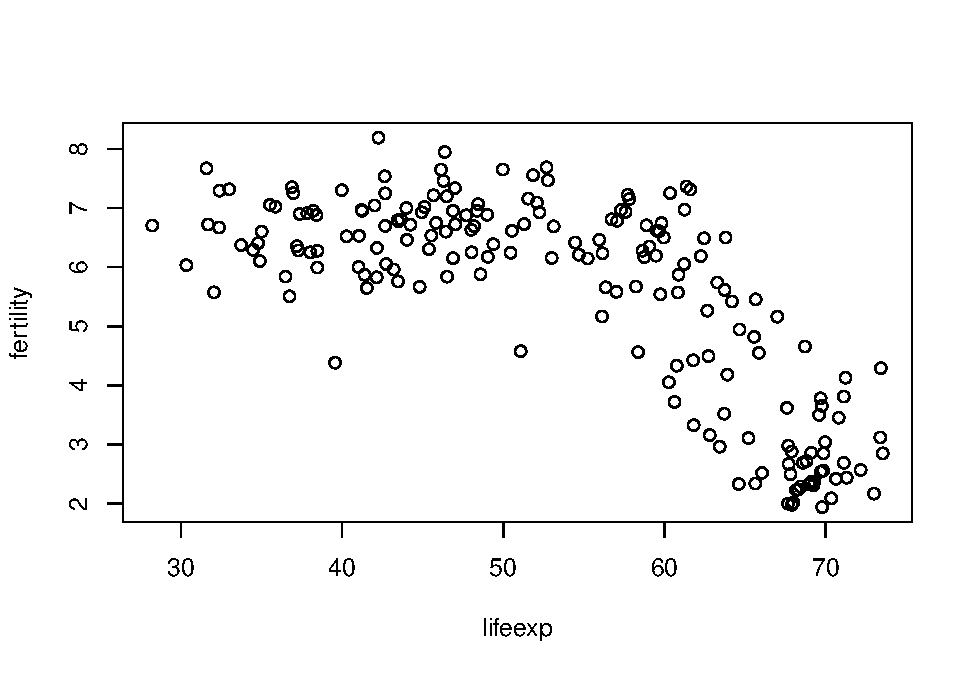
\includegraphics{stt-301-programming_files/figure-latex/unnamed-chunk-2-1.pdf}

\begin{Shaded}
\begin{Highlighting}[]
\NormalTok{pop <-}\StringTok{ }\NormalTok{WorldBank}\OperatorTok{$}\NormalTok{population[WorldBank}\OperatorTok{$}\NormalTok{year }\OperatorTok{==}\StringTok{ }\DecValTok{1960}\NormalTok{]}
\NormalTok{region <-}\StringTok{ }\NormalTok{WorldBank}\OperatorTok{$}\NormalTok{region[WorldBank}\OperatorTok{$}\NormalTok{year }\OperatorTok{==}\StringTok{ }\DecValTok{1960}\NormalTok{]}
\end{Highlighting}
\end{Shaded}

First we will create the axes, etc. for the plot, but not plot the
points, \texttt{type="n"} tells R to do this.

\begin{Shaded}
\begin{Highlighting}[]
\KeywordTok{plot}\NormalTok{(lifeexp, fertility, }\DataTypeTok{type=}\StringTok{"n"}\NormalTok{)}
\end{Highlighting}
\end{Shaded}

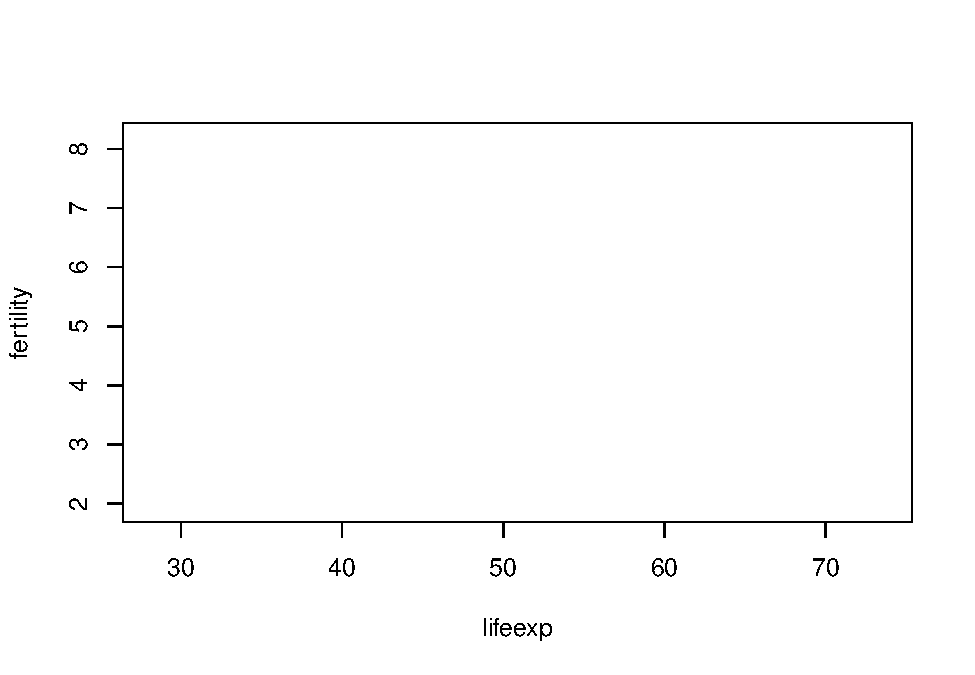
\includegraphics{stt-301-programming_files/figure-latex/unnamed-chunk-4-1.pdf}

\begin{Shaded}
\begin{Highlighting}[]
\KeywordTok{symbols}\NormalTok{(lifeexp, fertility, }\DataTypeTok{circles=}\KeywordTok{sqrt}\NormalTok{(pop}\OperatorTok{/}\NormalTok{pi), }\DataTypeTok{inches=}\FloatTok{0.35}\NormalTok{, }\DataTypeTok{bg=}\KeywordTok{match}\NormalTok{(region, }\KeywordTok{unique}\NormalTok{(region)))}
\end{Highlighting}
\end{Shaded}

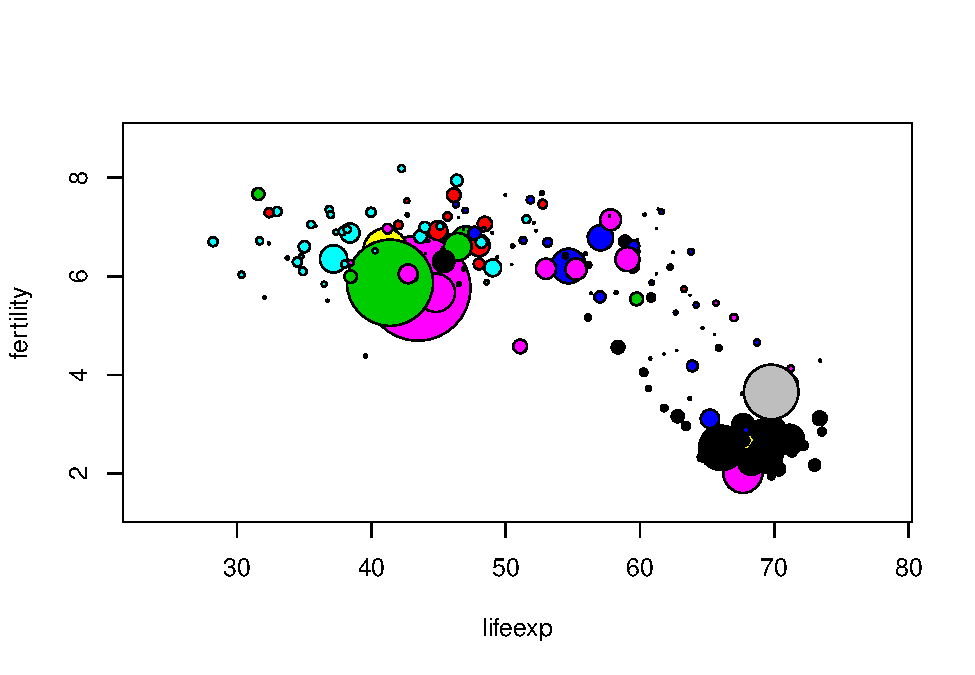
\includegraphics{stt-301-programming_files/figure-latex/unnamed-chunk-4-2.pdf}

\subsection{3.2 R Markdown}\label{r-markdown}

R Markdown provides a way to include R code that read in data, create
graphics, or perform analyses, in a single document which is processed
to create a research paper or homework assignment or other written
product.

\subsection{3.3 Basic formatting:}\label{basic-formatting}

\emph{italic} \textbf{bold} \textgreater{} block quote

\sout{strikethrough} A code chunk:

\begin{Shaded}
\begin{Highlighting}[]
\NormalTok{x <-}\StringTok{ }\DecValTok{1}\OperatorTok{:}\DecValTok{10}
\NormalTok{y <-}\StringTok{ }\DecValTok{10}\OperatorTok{:}\DecValTok{1}
\KeywordTok{mean}\NormalTok{(x)}
\end{Highlighting}
\end{Shaded}

\begin{verbatim}
## [1] 5.5
\end{verbatim}

\begin{Shaded}
\begin{Highlighting}[]
\KeywordTok{sd}\NormalTok{(y)}
\end{Highlighting}
\end{Shaded}

\begin{verbatim}
## [1] 3.02765
\end{verbatim}

Inline code: 10 Inline code not executed: \texttt{5+5}

\subsubsection{3.31 Text: Lists and
Headers}\label{text-lists-and-headers}

For an unordered list, either an asterisk, a plus sign, or a minus sign
may precede list items.

For an ordered list use a numeral followed by a period and a space (1.
or 2. or 3. or \ldots{}) For an ordered list, the first list item will
be labeled with the number or letter that you specify, but subsequent
list items will be numbered sequentially.

\textbf{An unordered list:}

\begin{itemize}
\tightlist
\item
  List item 1
\item
  List item 2

  \begin{itemize}
  \tightlist
  \item
    Second level list item 1
  \item
    Second level list item 2

    \begin{itemize}
    \tightlist
    \item
      Third level list item
    \end{itemize}
  \end{itemize}
\item
  List item 3
\end{itemize}

\textbf{An ordered list:}

\begin{enumerate}
\def\labelenumi{\arabic{enumi}.}
\tightlist
\item
  List item 1
\item
  List item 2

  \begin{enumerate}
  \def\labelenumii{\alph{enumii}.}
  \setcounter{enumii}{2}
  \tightlist
  \item
    Sub list item 1
  \item
    Sub list item 2
  \end{enumerate}
\item
  List item 3
\end{enumerate}

use \# to indicate headers.
\texttt{\#\ A\ first\ *level*\ \textasciitilde{}\textasciitilde{}header\textasciitilde{}\textasciitilde{}}
\texttt{\#\#\ A\ second\ level\ header}

\textbf{Text subscripts and superscripts:} x\textsubscript{2} +
y\textsubscript{2} 10\textsuperscript{3} = 1000 Mathematics examples:
\(x_a\)\\
\(x^a\)

\subsection{3.4 Code Chunks}\label{code-chunks}

\texttt{echo=FALSE} specifies that the R code should not be printed (but
any output of the R code should be printed) in the resulting document.

\begin{enumerate}
\def\labelenumi{\arabic{enumi}.}
\setcounter{enumi}{1}
\item
  \texttt{include=FALSE} specifies that neither the R code nor the
  output should be printed. However, the objects created by the code
  chunk will be available for use in later code chunks.
\item
  \texttt{eval=FALSE} specifies that the R code should not be evaluated.
  The code will be printed unless, for example, echo=FALSE is also given
  as an option.
\item
  error=FALSE and warning=FALSE specify that, respectively, error
  messages and warning messages generated by the R code should not be
  printed.
\item
  The \texttt{comment} option allows a specified character string to be
  prepended to each line of results. By default this is set to
  \texttt{comment\ =\ \#\#} which explains the two hash marks preceding
  results in Figure 3.3 for example. Setting \texttt{comment\ =\ NA}
  presents output without any character string prepended. That is done
  in most code chunks in this book.
\item
  \texttt{prompt=TRUE} specifies that R prompt \textgreater{} will be
  prepended to each line of R code shown in the document.
  \texttt{prompt\ =\ FALSE} specifies that command prompts should not be
  included.
\item
  \texttt{fig.height} and \texttt{fig.width} specify the height and
  width of figures generated by R code. These are specified in inches,
  so for example fig.height=4 specifies a four inch high figure.
\item
  \texttt{code} Set to R code. Knitr will replace the code in the chunk
  with the code in the code option.
\item
  \texttt{engine} `R' Knitr will evaluate the chunk in the named
  language, e.g.
  \texttt{engine\ =\ \textquotesingle{}python\textquotesingle{}}.
\item
  \texttt{collapse} If \texttt{TRUE}, knitr will collapse all the source
  and output blocks created by the chunk into a single block.
\item
  \texttt{results} `markup' If
  \texttt{\textquotesingle{}hide\textquotesingle{}}, knitr will not
  display the code's results in the final document. If
  \texttt{\textquotesingle{}hold\textquotesingle{}}, knitr will delay
  displaying all output pieces until the end of the chunk. If
  \texttt{\textquotesingle{}asis\textquotesingle{}}, knitr will pass
  through results without reformatting them (useful if results return
  raw HTML, etc.)
\item
  \texttt{error} If FALSE, knitr will not display any error messages
  generated by the code.
\item
  \texttt{message} If FALSE, knitr will not display any messages
  generated by the code.
\item
  \texttt{warning} If FALSE, knitr will not display any warning messages
  generated by the code.
\item
  \texttt{strip.white} If TRUE, knitr will remove white spaces that
  appear at the beginning or end of a code chunk.
\item
  \texttt{autodep} If TRUE, knitr will attempt to figure out
  dependencies between chunks automatically by analyzing object names.
\item
  \texttt{cache} If TRUE, knitr will cache the results to reuse in
  future knits. Knitr will reuse the results until the code chunk is
  altered.
\item
  \texttt{cache.comments} NULL If FALSE, knitr will not rerun the chunk
  if only a code comment has changed.
\end{enumerate}

\section{4.0 Data Structures}\label{data-structures}

\subsection{4.1 Vectors}\label{vectors}

Think of a vector as a structure to represent one variable in a data
set. For example

\textbf{Vectors in R can only contain elements of one type.} a vector
might hold the weights, in pounds, of 7 people in a data set.

\begin{Shaded}
\begin{Highlighting}[]
\NormalTok{weight <-}\StringTok{ }\KeywordTok{c}\NormalTok{(}\DecValTok{123}\NormalTok{, }\DecValTok{157}\NormalTok{, }\DecValTok{205}\NormalTok{, }\DecValTok{199}\NormalTok{, }\DecValTok{223}\NormalTok{, }\DecValTok{140}\NormalTok{, }\DecValTok{105}\NormalTok{)}
\NormalTok{weight}
\end{Highlighting}
\end{Shaded}

\begin{verbatim}
## [1] 123 157 205 199 223 140 105
\end{verbatim}

\begin{Shaded}
\begin{Highlighting}[]
\NormalTok{gender <-}\StringTok{ }\KeywordTok{c}\NormalTok{(}\StringTok{"female"}\NormalTok{, }\StringTok{"female"}\NormalTok{, }\StringTok{"male"}\NormalTok{, }\StringTok{"female"}\NormalTok{, }\StringTok{"male"}\NormalTok{, }\StringTok{"male"}\NormalTok{, }\StringTok{"female"}\NormalTok{)}
\NormalTok{gender}
\end{Highlighting}
\end{Shaded}

\begin{verbatim}
## [1] "female" "female" "male"   "female" "male"   "male"   "female"
\end{verbatim}

\textbf{Notice that elements of a vector are separated by commas when
using the \texttt{c()} function to create a vector.}

The \texttt{c()} function also can be used to add to an existing vector.
add at the last element.

\begin{Shaded}
\begin{Highlighting}[]
\NormalTok{weight <-}\StringTok{ }\KeywordTok{c}\NormalTok{(weight, }\DecValTok{194}\NormalTok{)}
\NormalTok{weight}
\end{Highlighting}
\end{Shaded}

\begin{verbatim}
## [1] 123 157 205 199 223 140 105 194
\end{verbatim}

\begin{Shaded}
\begin{Highlighting}[]
\NormalTok{gender <-}\StringTok{ }\KeywordTok{c}\NormalTok{(gender, }\StringTok{"male"}\NormalTok{)}

\NormalTok{gender}
\end{Highlighting}
\end{Shaded}

\begin{verbatim}
## [1] "female" "female" "male"   "female" "male"   "male"   "female" "male"
\end{verbatim}

\subsubsection{4.11 Types, conversion,
coercion}\label{types-conversion-coercion}

\begin{Shaded}
\begin{Highlighting}[]
\KeywordTok{typeof}\NormalTok{(weight)}
\end{Highlighting}
\end{Shaded}

\begin{verbatim}
## [1] "double"
\end{verbatim}

\begin{Shaded}
\begin{Highlighting}[]
\KeywordTok{typeof}\NormalTok{(gender)}
\end{Highlighting}
\end{Shaded}

\begin{verbatim}
## [1] "character"
\end{verbatim}

\begin{Shaded}
\begin{Highlighting}[]
\NormalTok{bp <-}\StringTok{ }\KeywordTok{c}\NormalTok{(}\OtherTok{FALSE}\NormalTok{, }\OtherTok{TRUE}\NormalTok{, }\OtherTok{FALSE}\NormalTok{, }\OtherTok{FALSE}\NormalTok{, }\OtherTok{TRUE}\NormalTok{, }\OtherTok{FALSE}\NormalTok{, }\OtherTok{TRUE}\NormalTok{, }\OtherTok{FALSE}\NormalTok{)}
\NormalTok{bp}
\end{Highlighting}
\end{Shaded}

\begin{verbatim}
## [1] FALSE  TRUE FALSE FALSE  TRUE FALSE  TRUE FALSE
\end{verbatim}

\begin{Shaded}
\begin{Highlighting}[]
\KeywordTok{typeof}\NormalTok{(bp)}
\end{Highlighting}
\end{Shaded}

\begin{verbatim}
## [1] "logical"
\end{verbatim}

\begin{Shaded}
\begin{Highlighting}[]
\KeywordTok{as.character}\NormalTok{(bp)}
\end{Highlighting}
\end{Shaded}

\begin{verbatim}
## [1] "FALSE" "TRUE"  "FALSE" "FALSE" "TRUE"  "FALSE" "TRUE"  "FALSE"
\end{verbatim}

\begin{Shaded}
\begin{Highlighting}[]
\KeywordTok{as.numeric}\NormalTok{(bp)}
\end{Highlighting}
\end{Shaded}

\begin{verbatim}
## [1] 0 1 0 0 1 0 1 0
\end{verbatim}

\begin{Shaded}
\begin{Highlighting}[]
\KeywordTok{is.character}\NormalTok{(bp)}
\end{Highlighting}
\end{Shaded}

\begin{verbatim}
## [1] FALSE
\end{verbatim}

\begin{Shaded}
\begin{Highlighting}[]
\NormalTok{char_bp =}\StringTok{ }\KeywordTok{as.character}\NormalTok{(bp)}
\KeywordTok{is.character}\NormalTok{(char_bp)}
\end{Highlighting}
\end{Shaded}

\begin{verbatim}
## [1] TRUE
\end{verbatim}

\begin{Shaded}
\begin{Highlighting}[]
\NormalTok{weight.int <-}\StringTok{ }\KeywordTok{as.integer}\NormalTok{(weight)}
\NormalTok{weight.int}
\end{Highlighting}
\end{Shaded}

\begin{verbatim}
## [1] 123 157 205 199 223 140 105 194
\end{verbatim}

\begin{Shaded}
\begin{Highlighting}[]
\NormalTok{weight.char <-}\StringTok{ }\KeywordTok{as.character}\NormalTok{(weight)}
\NormalTok{weight.char}
\end{Highlighting}
\end{Shaded}

\begin{verbatim}
## [1] "123" "157" "205" "199" "223" "140" "105" "194"
\end{verbatim}

\begin{Shaded}
\begin{Highlighting}[]
\NormalTok{bp.double <-}\StringTok{ }\KeywordTok{as.double}\NormalTok{(bp)}
\NormalTok{bp.double}
\end{Highlighting}
\end{Shaded}

\begin{verbatim}
## [1] 0 1 0 0 1 0 1 0
\end{verbatim}

\subsubsection{4.12 Coercion}\label{coercion}

Values are converted to the simplest type to represent all the
information \textbf{Character \textgreater{} complex \textgreater{}
double \textgreater{} integer \textgreater{} logical}

\begin{Shaded}
\begin{Highlighting}[]
\KeywordTok{c}\NormalTok{(}\DecValTok{4} \OperatorTok{+}\StringTok{ }\NormalTok{3i, }\OtherTok{TRUE}\NormalTok{, }\StringTok{"red"}\NormalTok{, }\DecValTok{6}\NormalTok{) }\CommentTok{# will become character}
\end{Highlighting}
\end{Shaded}

\begin{verbatim}
## [1] "4+3i" "TRUE" "red"  "6"
\end{verbatim}

\begin{Shaded}
\begin{Highlighting}[]
\KeywordTok{c}\NormalTok{(}\DecValTok{4} \OperatorTok{+}\StringTok{ }\NormalTok{3i, }\OtherTok{TRUE}\NormalTok{, }\DecValTok{4}\OperatorTok{/}\DecValTok{5}\NormalTok{, }\DecValTok{6}\NormalTok{) }\CommentTok{# will become complex}
\end{Highlighting}
\end{Shaded}

\begin{verbatim}
## [1] 4.0+3i 1.0+0i 0.8+0i 6.0+0i
\end{verbatim}

\begin{Shaded}
\begin{Highlighting}[]
\KeywordTok{c}\NormalTok{(}\DecValTok{4} \OperatorTok{+}\StringTok{ }\DecValTok{3}\NormalTok{, }\OtherTok{TRUE}\NormalTok{, }\DecValTok{4}\OperatorTok{/}\DecValTok{5}\NormalTok{, }\FloatTok{6.0}\NormalTok{) }\CommentTok{# will become double}
\end{Highlighting}
\end{Shaded}

\begin{verbatim}
## [1] 7.0 1.0 0.8 6.0
\end{verbatim}

\begin{Shaded}
\begin{Highlighting}[]
\KeywordTok{c}\NormalTok{(}\DecValTok{4} \OperatorTok{+}\StringTok{ }\DecValTok{3}\NormalTok{, }\OtherTok{TRUE}\NormalTok{, }\DecValTok{6}\NormalTok{) }\CommentTok{# will become Integer}
\end{Highlighting}
\end{Shaded}

\begin{verbatim}
## [1] 7 1 6
\end{verbatim}

\begin{Shaded}
\begin{Highlighting}[]
\NormalTok{yy <-}\StringTok{ }\KeywordTok{c}\NormalTok{(}\DecValTok{1}\NormalTok{, }\DecValTok{2}\NormalTok{, }\DecValTok{3}\NormalTok{, }\StringTok{"dog"}\NormalTok{)}
\NormalTok{yy}
\end{Highlighting}
\end{Shaded}

\begin{verbatim}
## [1] "1"   "2"   "3"   "dog"
\end{verbatim}

\subsubsection{4.13 Accessing specific elements of
vectors}\label{accessing-specific-elements-of-vectors}

\begin{Shaded}
\begin{Highlighting}[]
\NormalTok{weight[}\DecValTok{5}\NormalTok{]}
\end{Highlighting}
\end{Shaded}

\begin{verbatim}
## [1] 223
\end{verbatim}

\begin{Shaded}
\begin{Highlighting}[]
\NormalTok{weight[}\DecValTok{1}\OperatorTok{:}\DecValTok{3}\NormalTok{]}
\end{Highlighting}
\end{Shaded}

\begin{verbatim}
## [1] 123 157 205
\end{verbatim}

\begin{Shaded}
\begin{Highlighting}[]
\KeywordTok{length}\NormalTok{(weight)}
\end{Highlighting}
\end{Shaded}

\begin{verbatim}
## [1] 8
\end{verbatim}

\begin{Shaded}
\begin{Highlighting}[]
\NormalTok{weight[}\KeywordTok{length}\NormalTok{(weight)]}
\end{Highlighting}
\end{Shaded}

\begin{verbatim}
## [1] 194
\end{verbatim}

\begin{Shaded}
\begin{Highlighting}[]
\NormalTok{weight[}\DecValTok{3}\NormalTok{] <-}\StringTok{ }\DecValTok{200000}
\NormalTok{weight}
\end{Highlighting}
\end{Shaded}

\begin{verbatim}
## [1]    123    157 200000    199    223    140    105    194
\end{verbatim}

\textbf{Negative numbers in the square brackets tell R to omit the
corresponding value.}

\begin{Shaded}
\begin{Highlighting}[]
\NormalTok{weight[}\OperatorTok{-}\DecValTok{3}\NormalTok{]}
\end{Highlighting}
\end{Shaded}

\begin{verbatim}
## [1] 123 157 199 223 140 105 194
\end{verbatim}

\begin{Shaded}
\begin{Highlighting}[]
\NormalTok{lessWeight <-}\StringTok{ }\NormalTok{weight[}\OperatorTok{-}\KeywordTok{c}\NormalTok{(}\DecValTok{1}\NormalTok{, }\DecValTok{3}\NormalTok{, }\DecValTok{5}\NormalTok{)]}
\NormalTok{lessWeight}
\end{Highlighting}
\end{Shaded}

\begin{verbatim}
## [1] 157 199 140 105 194
\end{verbatim}

\begin{Shaded}
\begin{Highlighting}[]
\NormalTok{weight}
\end{Highlighting}
\end{Shaded}

\begin{verbatim}
## [1]    123    157 200000    199    223    140    105    194
\end{verbatim}

\subsection{4.2 Factors}\label{factors}

Categorical variables such as \texttt{gender} can be represented as
character vectors. In many cases this simple representation is
sufficient. \textbf{Factors in R provide a more sophisticated way to
represent categorical variables.}

\begin{Shaded}
\begin{Highlighting}[]
\NormalTok{age <-}\StringTok{ }\KeywordTok{c}\NormalTok{(}\StringTok{"middle age"}\NormalTok{, }\StringTok{"senior"}\NormalTok{, }\StringTok{"middle age"}\NormalTok{, }\StringTok{"senior"}\NormalTok{, }\StringTok{"senior"}\NormalTok{, }\StringTok{"senior"}\NormalTok{, }\StringTok{"senior"}\NormalTok{, }\StringTok{"middle age"}\NormalTok{)}
\NormalTok{age}
\end{Highlighting}
\end{Shaded}

\begin{verbatim}
## [1] "middle age" "senior"     "middle age" "senior"     "senior"    
## [6] "senior"     "senior"     "middle age"
\end{verbatim}

\begin{Shaded}
\begin{Highlighting}[]
\NormalTok{income <-}\StringTok{ }\KeywordTok{c}\NormalTok{(}\StringTok{"lower"}\NormalTok{, }\StringTok{"lower"}\NormalTok{, }\StringTok{"upper"}\NormalTok{, }\StringTok{"middle"}\NormalTok{, }\StringTok{"upper"}\NormalTok{, }\StringTok{"lower"}\NormalTok{, }\StringTok{"lower"}\NormalTok{, }\StringTok{"middle"}\NormalTok{)}
\NormalTok{income}
\end{Highlighting}
\end{Shaded}

\begin{verbatim}
## [1] "lower"  "lower"  "upper"  "middle" "upper"  "lower"  "lower"  "middle"
\end{verbatim}

\begin{Shaded}
\begin{Highlighting}[]
\NormalTok{age <-}\StringTok{ }\KeywordTok{factor}\NormalTok{(age, }\DataTypeTok{levels=}\KeywordTok{c}\NormalTok{(}\StringTok{"youth"}\NormalTok{, }\StringTok{"young adult"}\NormalTok{, }\StringTok{"middle age"}\NormalTok{, }\StringTok{"senior"}\NormalTok{))}
\NormalTok{age}
\end{Highlighting}
\end{Shaded}

\begin{verbatim}
## [1] middle age senior     middle age senior     senior     senior    
## [7] senior     middle age
## Levels: youth young adult middle age senior
\end{verbatim}

\begin{Shaded}
\begin{Highlighting}[]
\NormalTok{income <-}\StringTok{ }\KeywordTok{factor}\NormalTok{(income, }\DataTypeTok{levels=}\KeywordTok{c}\NormalTok{(}\StringTok{"lower"}\NormalTok{, }\StringTok{"middle"}\NormalTok{, }\StringTok{"upper"}\NormalTok{),}\DataTypeTok{ordered =} \OtherTok{TRUE}\NormalTok{)}
\NormalTok{income}
\end{Highlighting}
\end{Shaded}

\begin{verbatim}
## [1] lower  lower  upper  middle upper  lower  lower  middle
## Levels: lower < middle < upper
\end{verbatim}

\subsubsection{4.14 Vector Recycling}\label{vector-recycling}

\begin{Shaded}
\begin{Highlighting}[]
\NormalTok{x =}\StringTok{ }\KeywordTok{c}\NormalTok{(}\DecValTok{2}\NormalTok{,}\DecValTok{3}\NormalTok{,}\DecValTok{4}\NormalTok{)}
\NormalTok{y =}\StringTok{ }\KeywordTok{c}\NormalTok{(}\DecValTok{5}\NormalTok{,}\DecValTok{6}\NormalTok{,}\DecValTok{7}\NormalTok{)}
\NormalTok{y }\OperatorTok{+}\StringTok{ }\NormalTok{x}
\end{Highlighting}
\end{Shaded}

\begin{verbatim}
## [1]  7  9 11
\end{verbatim}

\begin{Shaded}
\begin{Highlighting}[]
\NormalTok{x_small =}\StringTok{ }\KeywordTok{c}\NormalTok{(}\DecValTok{1}\NormalTok{,}\DecValTok{2}\NormalTok{,}\DecValTok{3}\NormalTok{)}
\NormalTok{y_big =}\StringTok{ }\KeywordTok{c}\NormalTok{(}\DecValTok{1}\NormalTok{,}\DecValTok{2}\NormalTok{,}\DecValTok{3}\NormalTok{,}\DecValTok{4}\NormalTok{,}\DecValTok{5}\NormalTok{,}\DecValTok{6}\NormalTok{)}
 
\NormalTok{x_small }\OperatorTok{+}\StringTok{ }\NormalTok{y_big}
\end{Highlighting}
\end{Shaded}

\begin{verbatim}
## [1] 2 4 6 5 7 9
\end{verbatim}

\begin{Shaded}
\begin{Highlighting}[]
\NormalTok{x <-}\StringTok{ }\NormalTok{weight}
\NormalTok{x <-}\StringTok{ }\KeywordTok{c}\NormalTok{(x, }\OtherTok{NA}\NormalTok{, }\OtherTok{NA}\NormalTok{)}
\KeywordTok{sum}\NormalTok{(}\KeywordTok{is.na}\NormalTok{(x))}
\end{Highlighting}
\end{Shaded}

\begin{verbatim}
## [1] 2
\end{verbatim}

\begin{Shaded}
\begin{Highlighting}[]
\NormalTok{x[}\DecValTok{100}\NormalTok{]}
\end{Highlighting}
\end{Shaded}

\begin{verbatim}
## [1] NA
\end{verbatim}

\begin{Shaded}
\begin{Highlighting}[]
\NormalTok{x =}\StringTok{ }\DecValTok{1}\OperatorTok{:}\DecValTok{10}
\KeywordTok{mean}\NormalTok{(}\DataTypeTok{na.rm=}\OtherTok{FALSE}\NormalTok{, x, }\DataTypeTok{trim=}\DecValTok{0}\NormalTok{)}
\end{Highlighting}
\end{Shaded}

\begin{verbatim}
## [1] 5.5
\end{verbatim}

\begin{Shaded}
\begin{Highlighting}[]
\NormalTok{y <-}\StringTok{ }\NormalTok{mpg[, }\DecValTok{2}\NormalTok{]}
\end{Highlighting}
\end{Shaded}

\begin{Shaded}
\begin{Highlighting}[]
\KeywordTok{dim}\NormalTok{(mpg)}
\end{Highlighting}
\end{Shaded}

\begin{verbatim}
## [1] 234  11
\end{verbatim}

\begin{Shaded}
\begin{Highlighting}[]
\NormalTok{z <-}\StringTok{ }\KeywordTok{rep}\NormalTok{(}\DecValTok{0}\NormalTok{, }\DataTypeTok{length =} \KeywordTok{dim}\NormalTok{(mpg)[}\DecValTok{2}\NormalTok{])}
\ControlFlowTok{for}\NormalTok{ (i }\ControlFlowTok{in} \DecValTok{1}\OperatorTok{:}\KeywordTok{dim}\NormalTok{(mpg)[}\DecValTok{2}\NormalTok{])\{}
\NormalTok{    z[i] <-}\StringTok{ }\KeywordTok{sum}\NormalTok{(mpg[, i] }\OperatorTok{<}\StringTok{ }\DecValTok{5}\NormalTok{)\}}
\NormalTok{z}
\end{Highlighting}
\end{Shaded}

\begin{verbatim}
##  [1]   0   6 196   0  81   0 103   0   0   0   5
\end{verbatim}

\begin{Shaded}
\begin{Highlighting}[]
\NormalTok{a <-}\StringTok{ }\KeywordTok{c}\NormalTok{(}\DecValTok{3}\NormalTok{, }\DecValTok{6}\NormalTok{, }\DecValTok{9}\NormalTok{, }\DecValTok{12}\NormalTok{)}
\NormalTok{b <-}\StringTok{ }\KeywordTok{matrix}\NormalTok{(}\KeywordTok{c}\NormalTok{(}\DecValTok{1}\OperatorTok{:}\DecValTok{4}\NormalTok{), }\DataTypeTok{nrow =} \DecValTok{2}\NormalTok{, }\DataTypeTok{ncol =} \DecValTok{2}\NormalTok{)}
\NormalTok{c <-}\StringTok{ }\KeywordTok{c}\NormalTok{(}\StringTok{"good"}\NormalTok{, }\StringTok{"bad"}\NormalTok{, }\StringTok{"indifferent"}\NormalTok{)}
\NormalTok{my.list <-}\StringTok{ }\KeywordTok{list}\NormalTok{(a, b, c)}
\NormalTok{my.list}
\end{Highlighting}
\end{Shaded}

\begin{verbatim}
## [[1]]
## [1]  3  6  9 12
## 
## [[2]]
##      [,1] [,2]
## [1,]    1    3
## [2,]    2    4
## 
## [[3]]
## [1] "good"        "bad"         "indifferent"
\end{verbatim}

\begin{Shaded}
\begin{Highlighting}[]
\NormalTok{ my.list[[}\DecValTok{1}\NormalTok{]][}\DecValTok{3}\NormalTok{]}
\end{Highlighting}
\end{Shaded}

\begin{verbatim}
## [1] 9
\end{verbatim}

\begin{Shaded}
\begin{Highlighting}[]
\NormalTok{  my.list[[}\DecValTok{2}\NormalTok{]][}\DecValTok{2}\NormalTok{, ]}
\end{Highlighting}
\end{Shaded}

\begin{verbatim}
## [1] 2 4
\end{verbatim}

\subsection{4.3 Missing Data, Infinity,}\label{missing-data-infinity}

\begin{Shaded}
\begin{Highlighting}[]
\NormalTok{missingCharacter <-}\StringTok{ }\KeywordTok{c}\NormalTok{(}\StringTok{"dog"}\NormalTok{, }\StringTok{"cat"}\NormalTok{, }\OtherTok{NA}\NormalTok{, }\StringTok{"pig"}\NormalTok{, }\OtherTok{NA}\NormalTok{, }\StringTok{"horse"}\NormalTok{)}
\NormalTok{missingCharacter}
\end{Highlighting}
\end{Shaded}

\begin{verbatim}
## [1] "dog"   "cat"   NA      "pig"   NA      "horse"
\end{verbatim}

\begin{Shaded}
\begin{Highlighting}[]
\KeywordTok{is.na}\NormalTok{(missingCharacter)}
\end{Highlighting}
\end{Shaded}

\begin{verbatim}
## [1] FALSE FALSE  TRUE FALSE  TRUE FALSE
\end{verbatim}

\textbf{remove the missing value(s) and then perform the computation.}

\begin{Shaded}
\begin{Highlighting}[]
\KeywordTok{mean}\NormalTok{(}\KeywordTok{c}\NormalTok{(}\DecValTok{1}\NormalTok{, }\DecValTok{2}\NormalTok{, }\DecValTok{3}\NormalTok{, }\OtherTok{NA}\NormalTok{, }\DecValTok{5}\NormalTok{), }\DataTypeTok{na.rm =} \OtherTok{TRUE}\NormalTok{)}
\end{Highlighting}
\end{Shaded}

\begin{verbatim}
## [1] 2.75
\end{verbatim}

\textbf{1. NaN` represents the result of a calculation where the result
is undefined, such as dividing zero by zero.}

\textbf{2. \#\#\# Inf and -Inf represent infinity and negative infinity
(and numbers which are too large in magnitude to be represented as
floating point numbers).}

\subsection{4.5 Data Frames}\label{data-frames}

data is rectangular in form, with variables as columns and cases as
rows.

\begin{Shaded}
\begin{Highlighting}[]
\NormalTok{gender <-}\StringTok{ }\KeywordTok{c}\NormalTok{(}\StringTok{"female"}\NormalTok{, }\StringTok{"female"}\NormalTok{, }\StringTok{"male"}\NormalTok{, }\StringTok{"female"}\NormalTok{, }\StringTok{"male"}\NormalTok{, }\StringTok{"male"}\NormalTok{, }\StringTok{"female"}\NormalTok{)}
\NormalTok{bp <-}\StringTok{ }\KeywordTok{c}\NormalTok{(}\OtherTok{FALSE}\NormalTok{, }\OtherTok{TRUE}\NormalTok{, }\OtherTok{FALSE}\NormalTok{, }\OtherTok{FALSE}\NormalTok{, }\OtherTok{TRUE}\NormalTok{, }\OtherTok{FALSE}\NormalTok{, }\OtherTok{TRUE}\NormalTok{)}
\NormalTok{weight <-}\StringTok{ }\KeywordTok{c}\NormalTok{(}\DecValTok{123}\NormalTok{, }\DecValTok{157}\NormalTok{, }\DecValTok{205}\NormalTok{, }\DecValTok{199}\NormalTok{, }\DecValTok{223}\NormalTok{, }\DecValTok{140}\NormalTok{, }\DecValTok{105}\NormalTok{)}

\NormalTok{healthData <-}\StringTok{ }\KeywordTok{data.frame}\NormalTok{(}\DataTypeTok{Weight =}\NormalTok{ weight, }\DataTypeTok{Gender=}\NormalTok{gender, }\DataTypeTok{bp.meds =}\NormalTok{ bp,  }\DataTypeTok{stringsAsFactors=}\OtherTok{FALSE}\NormalTok{)}

\NormalTok{healthData}
\end{Highlighting}
\end{Shaded}

\begin{verbatim}
##   Weight Gender bp.meds
## 1    123 female   FALSE
## 2    157 female    TRUE
## 3    205   male   FALSE
## 4    199 female   FALSE
## 5    223   male    TRUE
## 6    140   male   FALSE
## 7    105 female    TRUE
\end{verbatim}

\begin{Shaded}
\begin{Highlighting}[]
\KeywordTok{names}\NormalTok{(healthData)}
\end{Highlighting}
\end{Shaded}

\begin{verbatim}
## [1] "Weight"  "Gender"  "bp.meds"
\end{verbatim}

\begin{Shaded}
\begin{Highlighting}[]
\KeywordTok{colnames}\NormalTok{(healthData)}
\end{Highlighting}
\end{Shaded}

\begin{verbatim}
## [1] "Weight"  "Gender"  "bp.meds"
\end{verbatim}

\begin{Shaded}
\begin{Highlighting}[]
\KeywordTok{names}\NormalTok{(healthData) <-}\StringTok{ }\KeywordTok{c}\NormalTok{(}\StringTok{"Wt"}\NormalTok{, }\StringTok{"Gdr"}\NormalTok{, }\StringTok{"bp"}\NormalTok{)}
\NormalTok{healthData}
\end{Highlighting}
\end{Shaded}

\begin{verbatim}
##    Wt    Gdr    bp
## 1 123 female FALSE
## 2 157 female  TRUE
## 3 205   male FALSE
## 4 199 female FALSE
## 5 223   male  TRUE
## 6 140   male FALSE
## 7 105 female  TRUE
\end{verbatim}

\begin{Shaded}
\begin{Highlighting}[]
\KeywordTok{rownames}\NormalTok{(healthData)}
\end{Highlighting}
\end{Shaded}

\begin{verbatim}
## [1] "1" "2" "3" "4" "5" "6" "7"
\end{verbatim}

\begin{Shaded}
\begin{Highlighting}[]
\KeywordTok{names}\NormalTok{(healthData) <-}\StringTok{ }\KeywordTok{c}\NormalTok{(}\StringTok{"Weight"}\NormalTok{, }\StringTok{"Gender"}\NormalTok{, }\StringTok{"bp.meds"}\NormalTok{)}
\NormalTok{healthData}
\end{Highlighting}
\end{Shaded}

\begin{verbatim}
##   Weight Gender bp.meds
## 1    123 female   FALSE
## 2    157 female    TRUE
## 3    205   male   FALSE
## 4    199 female   FALSE
## 5    223   male    TRUE
## 6    140   male   FALSE
## 7    105 female    TRUE
\end{verbatim}

\subsubsection{4.5.1 Accessing specific elements of data
frames}\label{accessing-specific-elements-of-data-frames}

Data frames are two-dimensional, so to access a specific element (or
elements) we need to specify both the row and column.

\begin{Shaded}
\begin{Highlighting}[]
\KeywordTok{data}\NormalTok{(mtcars)}
\KeywordTok{head}\NormalTok{(mtcars)}
\end{Highlighting}
\end{Shaded}

\begin{verbatim}
##                    mpg cyl disp  hp drat    wt  qsec vs am gear carb
## Mazda RX4         21.0   6  160 110 3.90 2.620 16.46  0  1    4    4
## Mazda RX4 Wag     21.0   6  160 110 3.90 2.875 17.02  0  1    4    4
## Datsun 710        22.8   4  108  93 3.85 2.320 18.61  1  1    4    1
## Hornet 4 Drive    21.4   6  258 110 3.08 3.215 19.44  1  0    3    1
## Hornet Sportabout 18.7   8  360 175 3.15 3.440 17.02  0  0    3    2
## Valiant           18.1   6  225 105 2.76 3.460 20.22  1  0    3    1
\end{verbatim}

\begin{Shaded}
\begin{Highlighting}[]
\NormalTok{mtcars[}\DecValTok{3}\NormalTok{, }\DecValTok{4}\NormalTok{]}
\end{Highlighting}
\end{Shaded}

\begin{verbatim}
## [1] 93
\end{verbatim}

\begin{Shaded}
\begin{Highlighting}[]
\KeywordTok{row.names}\NormalTok{(mtcars)}
\end{Highlighting}
\end{Shaded}

\begin{verbatim}
##  [1] "Mazda RX4"           "Mazda RX4 Wag"       "Datsun 710"         
##  [4] "Hornet 4 Drive"      "Hornet Sportabout"   "Valiant"            
##  [7] "Duster 360"          "Merc 240D"           "Merc 230"           
## [10] "Merc 280"            "Merc 280C"           "Merc 450SE"         
## [13] "Merc 450SL"          "Merc 450SLC"         "Cadillac Fleetwood" 
## [16] "Lincoln Continental" "Chrysler Imperial"   "Fiat 128"           
## [19] "Honda Civic"         "Toyota Corolla"      "Toyota Corona"      
## [22] "Dodge Challenger"    "AMC Javelin"         "Camaro Z28"         
## [25] "Pontiac Firebird"    "Fiat X1-9"           "Porsche 914-2"      
## [28] "Lotus Europa"        "Ford Pantera L"      "Ferrari Dino"       
## [31] "Maserati Bora"       "Volvo 142E"
\end{verbatim}

\begin{Shaded}
\begin{Highlighting}[]
\NormalTok{mtcars[}\DecValTok{1}\OperatorTok{:}\DecValTok{3}\NormalTok{, }\DecValTok{2}\OperatorTok{:}\DecValTok{3}\NormalTok{]}
\end{Highlighting}
\end{Shaded}

\begin{verbatim}
##               cyl disp
## Mazda RX4       6  160
## Mazda RX4 Wag   6  160
## Datsun 710      4  108
\end{verbatim}

\begin{Shaded}
\begin{Highlighting}[]
\NormalTok{mtcars[}\StringTok{"cyl"}\NormalTok{]}
\end{Highlighting}
\end{Shaded}

\begin{verbatim}
##                     cyl
## Mazda RX4             6
## Mazda RX4 Wag         6
## Datsun 710            4
## Hornet 4 Drive        6
## Hornet Sportabout     8
## Valiant               6
## Duster 360            8
## Merc 240D             4
## Merc 230              4
## Merc 280              6
## Merc 280C             6
## Merc 450SE            8
## Merc 450SL            8
## Merc 450SLC           8
## Cadillac Fleetwood    8
## Lincoln Continental   8
## Chrysler Imperial     8
## Fiat 128              4
## Honda Civic           4
## Toyota Corolla        4
## Toyota Corona         4
## Dodge Challenger      8
## AMC Javelin           8
## Camaro Z28            8
## Pontiac Firebird      8
## Fiat X1-9             4
## Porsche 914-2         4
## Lotus Europa          4
## Ford Pantera L        8
## Ferrari Dino          6
## Maserati Bora         8
## Volvo 142E            4
\end{verbatim}

\textbf{Note that mtcars{[},1{]} returns ALL elements in the first
column.}

\begin{Shaded}
\begin{Highlighting}[]
\NormalTok{mtcars[, }\DecValTok{1}\NormalTok{]}
\end{Highlighting}
\end{Shaded}

\begin{verbatim}
##  [1] 21.0 21.0 22.8 21.4 18.7 18.1 14.3 24.4 22.8 19.2 17.8 16.4 17.3 15.2
## [15] 10.4 10.4 14.7 32.4 30.4 33.9 21.5 15.5 15.2 13.3 19.2 27.3 26.0 30.4
## [29] 15.8 19.7 15.0 21.4
\end{verbatim}

\textbf{For a data frame there is another way to access specific
columns, using the \$ notation.}

\begin{Shaded}
\begin{Highlighting}[]
\NormalTok{mtcars}\OperatorTok{$}\NormalTok{mpg}
\end{Highlighting}
\end{Shaded}

\begin{verbatim}
##  [1] 21.0 21.0 22.8 21.4 18.7 18.1 14.3 24.4 22.8 19.2 17.8 16.4 17.3 15.2
## [15] 10.4 10.4 14.7 32.4 30.4 33.9 21.5 15.5 15.2 13.3 19.2 27.3 26.0 30.4
## [29] 15.8 19.7 15.0 21.4
\end{verbatim}

\subsection{4.6 Lists}\label{lists}

\begin{center}\rule{0.5\linewidth}{\linethickness}\end{center}

Technically a list is a vector, but one in which elements can be of
different types.

\begin{center}\rule{0.5\linewidth}{\linethickness}\end{center}

\textbf{Key Properties:}

\begin{itemize}
\tightlist
\item
  Heterogenous
\item
  Index by position/name \texttt{my\_list{[}{[}2{]}{]}}

  \begin{itemize}
  \tightlist
  \item
    \texttt{my\_list{[}2{]}} will return 2 element as list
  \end{itemize}
\item
  Index with multiple position and names
\item
  Have names
\end{itemize}

\begin{center}\rule{0.5\linewidth}{\linethickness}\end{center}

\textbf{\texttt{The\ lm\ function\ returns\ a\ list}}

\begin{Shaded}
\begin{Highlighting}[]
\NormalTok{mpgHpLinMod <-}\StringTok{ }\KeywordTok{lm}\NormalTok{(mpg }\OperatorTok{~}\StringTok{ }\NormalTok{hp, }\DataTypeTok{data =}\NormalTok{ mtcars)}
\KeywordTok{mode}\NormalTok{(mpgHpLinMod)}
\end{Highlighting}
\end{Shaded}

\begin{verbatim}
## [1] "list"
\end{verbatim}

\begin{Shaded}
\begin{Highlighting}[]
\KeywordTok{names}\NormalTok{(mpgHpLinMod)}
\end{Highlighting}
\end{Shaded}

\begin{verbatim}
##  [1] "coefficients"  "residuals"     "effects"       "rank"         
##  [5] "fitted.values" "assign"        "qr"            "df.residual"  
##  [9] "xlevels"       "call"          "terms"         "model"
\end{verbatim}

\begin{Shaded}
\begin{Highlighting}[]
\NormalTok{mpgHpLinMod}
\end{Highlighting}
\end{Shaded}

\begin{verbatim}
## 
## Call:
## lm(formula = mpg ~ hp, data = mtcars)
## 
## Coefficients:
## (Intercept)           hp  
##    30.09886     -0.06823
\end{verbatim}

\begin{Shaded}
\begin{Highlighting}[]
\NormalTok{mpgHpLinMod}\OperatorTok{$}\NormalTok{coefficients}
\end{Highlighting}
\end{Shaded}

\begin{verbatim}
## (Intercept)          hp 
## 30.09886054 -0.06822828
\end{verbatim}

The list function is used to create lists.

\begin{Shaded}
\begin{Highlighting}[]
\NormalTok{temporaryList <-}\StringTok{ }\KeywordTok{list}\NormalTok{(}\DataTypeTok{first=}\NormalTok{weight, }\DataTypeTok{second=}\NormalTok{healthData, }\DataTypeTok{pickle=}\KeywordTok{list}\NormalTok{(}\DataTypeTok{a =} \DecValTok{1}\OperatorTok{:}\DecValTok{10}\NormalTok{, }\DataTypeTok{b=}\NormalTok{healthData))}

\NormalTok{temporaryList}\OperatorTok{$}\NormalTok{first}
\end{Highlighting}
\end{Shaded}

\begin{verbatim}
## [1] 123 157 205 199 223 140 105
\end{verbatim}

\begin{Shaded}
\begin{Highlighting}[]
\NormalTok{temporaryList[[}\DecValTok{1}\NormalTok{]]}
\end{Highlighting}
\end{Shaded}

\begin{verbatim}
## [1] 123 157 205 199 223 140 105
\end{verbatim}

\begin{Shaded}
\begin{Highlighting}[]
\NormalTok{temporaryList[[}\DecValTok{1}\NormalTok{]][}\DecValTok{1}\NormalTok{]}
\end{Highlighting}
\end{Shaded}

\begin{verbatim}
## [1] 123
\end{verbatim}

\begin{Shaded}
\begin{Highlighting}[]
\NormalTok{temporaryList}\OperatorTok{$}\NormalTok{second}
\end{Highlighting}
\end{Shaded}

\begin{verbatim}
##   Weight Gender bp.meds
## 1    123 female   FALSE
## 2    157 female    TRUE
## 3    205   male   FALSE
## 4    199 female   FALSE
## 5    223   male    TRUE
## 6    140   male   FALSE
## 7    105 female    TRUE
\end{verbatim}

\begin{Shaded}
\begin{Highlighting}[]
\NormalTok{temporaryList[}\KeywordTok{c}\NormalTok{(}\DecValTok{1}\NormalTok{, }\DecValTok{2}\NormalTok{)] }\CommentTok{# returns a list with 1st and 2nd elements}
\end{Highlighting}
\end{Shaded}

\begin{verbatim}
## $first
## [1] 123 157 205 199 223 140 105
## 
## $second
##   Weight Gender bp.meds
## 1    123 female   FALSE
## 2    157 female    TRUE
## 3    205   male   FALSE
## 4    199 female   FALSE
## 5    223   male    TRUE
## 6    140   male   FALSE
## 7    105 female    TRUE
\end{verbatim}

\begin{Shaded}
\begin{Highlighting}[]
\NormalTok{temporaryList[[}\KeywordTok{c}\NormalTok{(}\DecValTok{1}\NormalTok{, }\DecValTok{2}\NormalTok{)]]}
\end{Highlighting}
\end{Shaded}

\begin{verbatim}
## [1] 157
\end{verbatim}

\begin{Shaded}
\begin{Highlighting}[]
\NormalTok{temporaryList[}\DecValTok{2}\NormalTok{]}
\end{Highlighting}
\end{Shaded}

\begin{verbatim}
## $second
##   Weight Gender bp.meds
## 1    123 female   FALSE
## 2    157 female    TRUE
## 3    205   male   FALSE
## 4    199 female   FALSE
## 5    223   male    TRUE
## 6    140   male   FALSE
## 7    105 female    TRUE
\end{verbatim}

\begin{Shaded}
\begin{Highlighting}[]
\NormalTok{my_list =}\StringTok{ }\KeywordTok{list}\NormalTok{(}\DecValTok{1}\NormalTok{, }\DecValTok{2}\NormalTok{, }\DecValTok{3}\NormalTok{, }\KeywordTok{c}\NormalTok{(}\DecValTok{3}\NormalTok{, }\DecValTok{5}\NormalTok{, }\DecValTok{6}\NormalTok{), }\KeywordTok{c}\NormalTok{(}\StringTok{"a"}\NormalTok{, }\StringTok{"b"}\NormalTok{, }\StringTok{"c"}\NormalTok{))}
\NormalTok{my_list[}\DecValTok{1}\NormalTok{]}
\end{Highlighting}
\end{Shaded}

\begin{verbatim}
## [[1]]
## [1] 1
\end{verbatim}

\begin{Shaded}
\begin{Highlighting}[]
\NormalTok{my_list[[}\DecValTok{4}\NormalTok{]][}\DecValTok{1}\NormalTok{]}
\end{Highlighting}
\end{Shaded}

\begin{verbatim}
## [1] 3
\end{verbatim}

\begin{Shaded}
\begin{Highlighting}[]
\NormalTok{my_list[[}\KeywordTok{c}\NormalTok{(}\DecValTok{4}\NormalTok{, }\DecValTok{2}\NormalTok{)]]}
\end{Highlighting}
\end{Shaded}

\begin{verbatim}
## [1] 5
\end{verbatim}

\subsection{4.7 Subsetting with logical
vectors}\label{subsetting-with-logical-vectors}

\begin{Shaded}
\begin{Highlighting}[]
\NormalTok{weight}
\end{Highlighting}
\end{Shaded}

\begin{verbatim}
## [1] 123 157 205 199 223 140 105
\end{verbatim}

\begin{Shaded}
\begin{Highlighting}[]
\NormalTok{gender}
\end{Highlighting}
\end{Shaded}

\begin{verbatim}
## [1] "female" "female" "male"   "female" "male"   "male"   "female"
\end{verbatim}

\begin{Shaded}
\begin{Highlighting}[]
\NormalTok{gender[weight }\OperatorTok{>}\StringTok{ }\DecValTok{200}\NormalTok{]}
\end{Highlighting}
\end{Shaded}

\begin{verbatim}
## [1] "male" "male"
\end{verbatim}

\subsubsection{4.7.1 Modifying or creating objects via
subsetting}\label{modifying-or-creating-objects-via-subsetting}

\begin{Shaded}
\begin{Highlighting}[]
\NormalTok{lightweight <-}\StringTok{ }\NormalTok{weight[weight }\OperatorTok{<}\StringTok{ }\DecValTok{200}\NormalTok{]}
\NormalTok{lightweight}
\end{Highlighting}
\end{Shaded}

\begin{verbatim}
## [1] 123 157 199 140 105
\end{verbatim}

\begin{Shaded}
\begin{Highlighting}[]
\NormalTok{x <-}\StringTok{ }\DecValTok{1}\OperatorTok{:}\DecValTok{10}
\NormalTok{x}
\end{Highlighting}
\end{Shaded}

\begin{verbatim}
##  [1]  1  2  3  4  5  6  7  8  9 10
\end{verbatim}

\begin{Shaded}
\begin{Highlighting}[]
\NormalTok{x[x }\OperatorTok{<}\StringTok{ }\DecValTok{5}\NormalTok{] <-}\StringTok{ }\DecValTok{0}
\NormalTok{x}
\end{Highlighting}
\end{Shaded}

\begin{verbatim}
##  [1]  0  0  0  0  5  6  7  8  9 10
\end{verbatim}

\subsubsection{4.7.2 Logical subsetting and data
frames}\label{logical-subsetting-and-data-frames}

Example:

\begin{Shaded}
\begin{Highlighting}[]
\NormalTok{x =}\StringTok{ }\KeywordTok{c}\NormalTok{(}\OperatorTok{-}\DecValTok{3}\OperatorTok{:}\DecValTok{3}\NormalTok{)}
\NormalTok{x}
\end{Highlighting}
\end{Shaded}

\begin{verbatim}
## [1] -3 -2 -1  0  1  2  3
\end{verbatim}

\begin{Shaded}
\begin{Highlighting}[]
\NormalTok{z <-}\StringTok{ }\KeywordTok{c}\NormalTok{(T, F, F, T, F, F, F)}
\NormalTok{x[z]}
\end{Highlighting}
\end{Shaded}

\begin{verbatim}
## [1] -3  0
\end{verbatim}

** We can use
\texttt{\textless{},\ \textgreater{},\ ==,\ \textgreater{}=,\ \textless{}=\ !=}
to create conditions with \texttt{\&} and \texttt{I} **

\begin{Shaded}
\begin{Highlighting}[]
\NormalTok{healthData}
\end{Highlighting}
\end{Shaded}

\begin{verbatim}
##   Weight Gender bp.meds
## 1    123 female   FALSE
## 2    157 female    TRUE
## 3    205   male   FALSE
## 4    199 female   FALSE
## 5    223   male    TRUE
## 6    140   male   FALSE
## 7    105 female    TRUE
\end{verbatim}

\begin{Shaded}
\begin{Highlighting}[]
\NormalTok{healthData}\OperatorTok{$}\NormalTok{Weight[healthData}\OperatorTok{$}\NormalTok{Gender }\OperatorTok{==}\StringTok{ "male"}\NormalTok{]}
\end{Highlighting}
\end{Shaded}

\begin{verbatim}
## [1] 205 223 140
\end{verbatim}

\begin{Shaded}
\begin{Highlighting}[]
\NormalTok{healthData[healthData}\OperatorTok{$}\NormalTok{Weight }\OperatorTok{>}\StringTok{ }\DecValTok{190}\NormalTok{, }\DecValTok{2}\OperatorTok{:}\DecValTok{3}\NormalTok{]}
\end{Highlighting}
\end{Shaded}

\begin{verbatim}
##   Gender bp.meds
## 3   male   FALSE
## 4 female   FALSE
## 5   male    TRUE
\end{verbatim}

\begin{Shaded}
\begin{Highlighting}[]
\NormalTok{temporaryDataFrame <-}\StringTok{ }\KeywordTok{data.frame}\NormalTok{(}\DataTypeTok{V1 =} \KeywordTok{c}\NormalTok{(}\DecValTok{1}\NormalTok{, }\DecValTok{2}\NormalTok{, }\DecValTok{3}\NormalTok{, }\DecValTok{4}\NormalTok{, }\OtherTok{NA}\NormalTok{), }\DataTypeTok{V2 =} \KeywordTok{c}\NormalTok{(}\OtherTok{NA}\NormalTok{, }\DecValTok{1}\NormalTok{, }\DecValTok{4}\NormalTok{, }\DecValTok{5}\NormalTok{, }\OtherTok{NA}\NormalTok{), }\DataTypeTok{V3 =} \KeywordTok{c}\NormalTok{(}\DecValTok{1}\NormalTok{, }\DecValTok{2}\NormalTok{, }\DecValTok{3}\NormalTok{, }\DecValTok{5}\NormalTok{, }\DecValTok{7}\NormalTok{))}
\NormalTok{temporaryDataFrame}
\end{Highlighting}
\end{Shaded}

\begin{verbatim}
##   V1 V2 V3
## 1  1 NA  1
## 2  2  1  2
## 3  3  4  3
## 4  4  5  5
## 5 NA NA  7
\end{verbatim}

\begin{Shaded}
\begin{Highlighting}[]
\KeywordTok{is.na}\NormalTok{(temporaryDataFrame)}
\end{Highlighting}
\end{Shaded}

\begin{verbatim}
##         V1    V2    V3
## [1,] FALSE  TRUE FALSE
## [2,] FALSE FALSE FALSE
## [3,] FALSE FALSE FALSE
## [4,] FALSE FALSE FALSE
## [5,]  TRUE  TRUE FALSE
\end{verbatim}

\begin{Shaded}
\begin{Highlighting}[]
\KeywordTok{rowSums}\NormalTok{(}\KeywordTok{is.na}\NormalTok{(temporaryDataFrame))}
\end{Highlighting}
\end{Shaded}

\begin{verbatim}
## [1] 1 0 0 0 2
\end{verbatim}

\begin{Shaded}
\begin{Highlighting}[]
\KeywordTok{colSums}\NormalTok{(}\KeywordTok{is.na}\NormalTok{(temporaryDataFrame))}
\end{Highlighting}
\end{Shaded}

\begin{verbatim}
## V1 V2 V3 
##  1  2  0
\end{verbatim}

\subsection{4.8 Patterned data}\label{patterned-data}

The seq() function generates either a sequence of pre-specified length
or a sequence with pre-specified increments.

\begin{Shaded}
\begin{Highlighting}[]
\KeywordTok{seq}\NormalTok{(}\DataTypeTok{from =} \DecValTok{0}\NormalTok{, }\DataTypeTok{to =} \DecValTok{1}\NormalTok{, }\DataTypeTok{length =} \DecValTok{11}\NormalTok{)}
\end{Highlighting}
\end{Shaded}

\begin{verbatim}
##  [1] 0.0 0.1 0.2 0.3 0.4 0.5 0.6 0.7 0.8 0.9 1.0
\end{verbatim}

\begin{Shaded}
\begin{Highlighting}[]
\KeywordTok{seq}\NormalTok{(}\DataTypeTok{from =} \DecValTok{1}\NormalTok{, }\DataTypeTok{to =} \DecValTok{5}\NormalTok{, }\DataTypeTok{by =} \DecValTok{1}\OperatorTok{/}\DecValTok{3}\NormalTok{)}
\end{Highlighting}
\end{Shaded}

\begin{verbatim}
##  [1] 1.000000 1.333333 1.666667 2.000000 2.333333 2.666667 3.000000
##  [8] 3.333333 3.666667 4.000000 4.333333 4.666667 5.000000
\end{verbatim}

The rep() function replicates the values in a given vector.

\begin{Shaded}
\begin{Highlighting}[]
\KeywordTok{rep}\NormalTok{(}\KeywordTok{c}\NormalTok{(}\DecValTok{1}\NormalTok{, }\DecValTok{2}\NormalTok{, }\DecValTok{4}\NormalTok{), }\DataTypeTok{length =} \DecValTok{9}\NormalTok{)}
\end{Highlighting}
\end{Shaded}

\begin{verbatim}
## [1] 1 2 4 1 2 4 1 2 4
\end{verbatim}

\begin{Shaded}
\begin{Highlighting}[]
\KeywordTok{rep}\NormalTok{(}\KeywordTok{c}\NormalTok{(}\DecValTok{1}\NormalTok{, }\DecValTok{2}\NormalTok{, }\DecValTok{4}\NormalTok{), }\DataTypeTok{times =} \DecValTok{3}\NormalTok{)}
\end{Highlighting}
\end{Shaded}

\begin{verbatim}
## [1] 1 2 4 1 2 4 1 2 4
\end{verbatim}

\begin{Shaded}
\begin{Highlighting}[]
\KeywordTok{rep}\NormalTok{(}\KeywordTok{c}\NormalTok{(}\StringTok{"a"}\NormalTok{, }\StringTok{"b"}\NormalTok{, }\StringTok{"c"}\NormalTok{), }\DataTypeTok{times =} \KeywordTok{c}\NormalTok{(}\DecValTok{3}\NormalTok{, }\DecValTok{2}\NormalTok{, }\DecValTok{7}\NormalTok{))}
\end{Highlighting}
\end{Shaded}

\begin{verbatim}
##  [1] "a" "a" "a" "b" "b" "c" "c" "c" "c" "c" "c" "c"
\end{verbatim}

\section{Functions and Programming}\label{functions-and-programming}

Learning about R's programming capabilities is an important step in
gaining facility with functions.

\subsection{7.1 R functions}\label{r-functions}

\begin{Shaded}
\begin{Highlighting}[]
\NormalTok{u.corn <-}\StringTok{ "http://blue.for.msu.edu/FOR875/data/corn.csv"}
\NormalTok{corn <-}\StringTok{ }\KeywordTok{read.csv}\NormalTok{(u.corn, }\DataTypeTok{header =} \OtherTok{TRUE}\NormalTok{)}
\NormalTok{corn}
\end{Highlighting}
\end{Shaded}

\begin{verbatim}
##    regular kiln_dried
## 1     1903       2009
## 2     1935       1915
## 3     1910       2011
## 4     2496       2463
## 5     2108       2180
## 6     1961       1925
## 7     2060       2122
## 8     1444       1482
## 9     1612       1542
## 10    1316       1443
## 11    1511       1535
\end{verbatim}

\begin{Shaded}
\begin{Highlighting}[]
\NormalTok{paired_t <-}\StringTok{ }\ControlFlowTok{function}\NormalTok{(x1, x2) \{}
\NormalTok{  n <-}\StringTok{ }\KeywordTok{length}\NormalTok{(x1)}
\NormalTok{  dbar <-}\StringTok{ }\KeywordTok{mean}\NormalTok{(x1 }\OperatorTok{-}\StringTok{ }\NormalTok{x2)}
\NormalTok{  s_d <-}\StringTok{ }\KeywordTok{sd}\NormalTok{(x1 }\OperatorTok{-}\StringTok{ }\NormalTok{x2)}
\NormalTok{  tstat <-}\StringTok{ }\NormalTok{dbar}\OperatorTok{/}\NormalTok{(s_d}\OperatorTok{/}\KeywordTok{sqrt}\NormalTok{(n))}
\NormalTok{  pval <-}\StringTok{ }\DecValTok{2} \OperatorTok{*}\StringTok{ }\NormalTok{(}\DecValTok{1} \OperatorTok{-}\StringTok{ }\KeywordTok{pt}\NormalTok{(}\KeywordTok{abs}\NormalTok{(tstat), n }\OperatorTok{-}\StringTok{ }\DecValTok{1}\NormalTok{))}
\NormalTok{  margin <-}\StringTok{ }\KeywordTok{qt}\NormalTok{(}\FloatTok{0.975}\NormalTok{, n }\OperatorTok{-}\StringTok{ }\DecValTok{1}\NormalTok{) }\OperatorTok{*}\StringTok{ }\NormalTok{s_d}\OperatorTok{/}\KeywordTok{sqrt}\NormalTok{(n)}
\NormalTok{  lcl <-}\StringTok{ }\NormalTok{dbar }\OperatorTok{-}\StringTok{ }\NormalTok{margin}
\NormalTok{  ucl <-}\StringTok{ }\NormalTok{dbar }\OperatorTok{+}\StringTok{ }\NormalTok{margin}
  \KeywordTok{return}\NormalTok{(}\KeywordTok{list}\NormalTok{(}\DataTypeTok{tstat =}\NormalTok{ tstat, }\DataTypeTok{pval =}\NormalTok{ pval, }\DataTypeTok{lcl =}\NormalTok{ lcl, }\DataTypeTok{ucl =}\NormalTok{ ucl))}
\NormalTok{\}}

\KeywordTok{paired_t}\NormalTok{(}\DataTypeTok{x1 =}\NormalTok{ corn}\OperatorTok{$}\NormalTok{kiln_dried, }\DataTypeTok{x2 =}\NormalTok{ corn}\OperatorTok{$}\NormalTok{regular)}
\end{Highlighting}
\end{Shaded}

\begin{verbatim}
## $tstat
## [1] 1.690476
## 
## $pval
## [1] 0.1218166
## 
## $lcl
## [1] -10.7271
## 
## $ucl
## [1] 78.18164
\end{verbatim}

\subsubsection{7.1.1 Creating functions}\label{creating-functions}

A function can be written in any text editor, saved as a plain text file
(possibly with a .r extension), and then read into R using the source()
function.

\subsection{7.2 Programming: Conditional
Statements}\label{programming-conditional-statements}

The argument to the \texttt{if()} function is evaluated. If the argument
returns \texttt{TRUE} the ensuing code is executed.

\subsubsection{7.2.1 Comparison and logical
operators}\label{comparison-and-logical-operators}

\begin{Shaded}
\begin{Highlighting}[]
\KeywordTok{c}\NormalTok{(}\OtherTok{FALSE}\NormalTok{, }\OtherTok{TRUE}\NormalTok{, }\OtherTok{FALSE}\NormalTok{) }\OperatorTok{||}\StringTok{ }\KeywordTok{c}\NormalTok{(}\OtherTok{TRUE}\NormalTok{, }\OtherTok{FALSE}\NormalTok{, }\OtherTok{FALSE}\NormalTok{)}
\end{Highlighting}
\end{Shaded}

\begin{verbatim}
## [1] TRUE
\end{verbatim}

\begin{Shaded}
\begin{Highlighting}[]
\KeywordTok{c}\NormalTok{(}\OtherTok{FALSE}\NormalTok{, }\OtherTok{TRUE}\NormalTok{, }\OtherTok{FALSE}\NormalTok{) }\OperatorTok{|}\StringTok{ }\KeywordTok{c}\NormalTok{(}\OtherTok{TRUE}\NormalTok{, }\OtherTok{FALSE}\NormalTok{, }\OtherTok{FALSE}\NormalTok{)}
\end{Highlighting}
\end{Shaded}

\begin{verbatim}
## [1]  TRUE  TRUE FALSE
\end{verbatim}

\begin{Shaded}
\begin{Highlighting}[]
\KeywordTok{c}\NormalTok{(}\OtherTok{FALSE}\NormalTok{, }\OtherTok{TRUE}\NormalTok{, }\OtherTok{FALSE}\NormalTok{) }\OperatorTok{&&}\StringTok{ }\KeywordTok{c}\NormalTok{(}\OtherTok{TRUE}\NormalTok{, }\OtherTok{TRUE}\NormalTok{, }\OtherTok{FALSE}\NormalTok{)}
\end{Highlighting}
\end{Shaded}

\begin{verbatim}
## [1] FALSE
\end{verbatim}

\begin{Shaded}
\begin{Highlighting}[]
\KeywordTok{c}\NormalTok{(}\OtherTok{FALSE}\NormalTok{, }\OtherTok{TRUE}\NormalTok{, }\OtherTok{FALSE}\NormalTok{) }\OperatorTok{&}\StringTok{ }\KeywordTok{c}\NormalTok{(}\OtherTok{TRUE}\NormalTok{, }\OtherTok{TRUE}\NormalTok{, }\OtherTok{FALSE}\NormalTok{)}
\end{Highlighting}
\end{Shaded}

\begin{verbatim}
## [1] FALSE  TRUE FALSE
\end{verbatim}

\subsubsection{7.2.2 If else statements}\label{if-else-statements}

\begin{Shaded}
\begin{Highlighting}[]
\NormalTok{Sign <-}\StringTok{ }\ControlFlowTok{function}\NormalTok{(x) \{}
  \ControlFlowTok{if}\NormalTok{ (x }\OperatorTok{<}\StringTok{ }\DecValTok{0}\NormalTok{) \{}
     \KeywordTok{print}\NormalTok{(}\StringTok{"the number is negative"}\NormalTok{)}
\NormalTok{  \}}\ControlFlowTok{else} \ControlFlowTok{if}\NormalTok{ (x }\OperatorTok{>}\StringTok{ }\DecValTok{0}\NormalTok{) \{}
    \KeywordTok{print}\NormalTok{(}\StringTok{"the number is positive"}\NormalTok{)}
\NormalTok{  \}}\ControlFlowTok{else}\NormalTok{ \{}
    \KeywordTok{print}\NormalTok{(}\StringTok{"the number is zero"}\NormalTok{)}
\NormalTok{  \}}
\NormalTok{\}}
\KeywordTok{Sign}\NormalTok{(}\DecValTok{3}\NormalTok{)}
\end{Highlighting}
\end{Shaded}

\begin{verbatim}
## [1] "the number is positive"
\end{verbatim}

\begin{Shaded}
\begin{Highlighting}[]
\KeywordTok{Sign}\NormalTok{(}\OperatorTok{-}\DecValTok{3}\NormalTok{)}
\end{Highlighting}
\end{Shaded}

\begin{verbatim}
## [1] "the number is negative"
\end{verbatim}

\begin{Shaded}
\begin{Highlighting}[]
\KeywordTok{Sign}\NormalTok{(}\DecValTok{0}\NormalTok{)}
\end{Highlighting}
\end{Shaded}

\begin{verbatim}
## [1] "the number is zero"
\end{verbatim}

\subsection{7.3 Computer Arithmetic}\label{computer-arithmetic}

R does not perform exact arithmetic

\begin{Shaded}
\begin{Highlighting}[]
\DecValTok{2}\OperatorTok{^-}\DecValTok{30}
\end{Highlighting}
\end{Shaded}

\begin{verbatim}
## [1] 9.313226e-10
\end{verbatim}

\begin{Shaded}
\begin{Highlighting}[]
\DecValTok{2}\OperatorTok{^-}\DecValTok{30} \OperatorTok{+}\StringTok{ }\NormalTok{(}\DecValTok{2}\OperatorTok{^}\DecValTok{30} \OperatorTok{-}\StringTok{ }\DecValTok{2}\OperatorTok{^}\DecValTok{30}\NormalTok{)}
\end{Highlighting}
\end{Shaded}

\begin{verbatim}
## [1] 9.313226e-10
\end{verbatim}

\begin{Shaded}
\begin{Highlighting}[]
\NormalTok{(}\DecValTok{2}\OperatorTok{^-}\DecValTok{30} \OperatorTok{+}\StringTok{ }\DecValTok{2}\OperatorTok{^}\DecValTok{30}\NormalTok{) }\OperatorTok{-}\StringTok{ }\DecValTok{2}\OperatorTok{^}\DecValTok{30}
\end{Highlighting}
\end{Shaded}

\begin{verbatim}
## [1] 0
\end{verbatim}

\begin{Shaded}
\begin{Highlighting}[]
\FloatTok{1.5} \OperatorTok{-}\StringTok{ }\FloatTok{1.4} \OperatorTok{==}\StringTok{ }\FloatTok{0.1}
\end{Highlighting}
\end{Shaded}

\begin{verbatim}
## [1] FALSE
\end{verbatim}

\begin{Shaded}
\begin{Highlighting}[]
\KeywordTok{all.equal}\NormalTok{((}\FloatTok{1.5} \OperatorTok{-}\StringTok{ }\FloatTok{1.4}\NormalTok{), }\FloatTok{0.1}\NormalTok{)}
\end{Highlighting}
\end{Shaded}

\begin{verbatim}
## [1] TRUE
\end{verbatim}

\subsection{7.4 Loops}\label{loops}

Loops are an important component of any programming language, including
R. Vectorized calculations and functions such as apply() make loops a
bit less central to R than to many other languages.

\subsubsection{7.4.1 A repeat loop}\label{a-repeat-loop}

A \texttt{repeat\ loop} just repeats a given expression over and over
again until a break statement is encountered.

\begin{Shaded}
\begin{Highlighting}[]
\NormalTok{k <-}\StringTok{ }\DecValTok{1}
\ControlFlowTok{repeat}\NormalTok{ \{}
  \ControlFlowTok{if}\NormalTok{ (}\DecValTok{1} \OperatorTok{==}\StringTok{ }\DecValTok{1} \OperatorTok{+}\StringTok{ }\DecValTok{1}\OperatorTok{/}\DecValTok{2}\OperatorTok{^}\NormalTok{k)\{}
    \ControlFlowTok{break}
\NormalTok{  \}}\ControlFlowTok{else}\NormalTok{ \{}
\NormalTok{    k <-}\StringTok{ }\NormalTok{k }\OperatorTok{+}\StringTok{ }\DecValTok{1}
\NormalTok{  \}}
\NormalTok{\}}
\NormalTok{k}
\end{Highlighting}
\end{Shaded}

\begin{verbatim}
## [1] 53
\end{verbatim}

\subsubsection{7.4.2 A while loop}\label{a-while-loop}

A while loop has the form \texttt{while\ (condition)\ expression} As
long as the condition is \texttt{TRUE} the expression is evaluated. Once
the condition is \texttt{FALSE} control is transferred outside the loop.

\begin{Shaded}
\begin{Highlighting}[]
\NormalTok{k <-}\StringTok{ }\DecValTok{1}
\ControlFlowTok{while}\NormalTok{ (}\DecValTok{1} \OperatorTok{!=}\StringTok{ }\DecValTok{1} \OperatorTok{+}\StringTok{ }\DecValTok{1}\OperatorTok{/}\DecValTok{2}\OperatorTok{^}\NormalTok{k) \{}
\NormalTok{  k <-}\StringTok{ }\NormalTok{k }\OperatorTok{+}\StringTok{ }\DecValTok{1}
\NormalTok{\}}
\NormalTok{k}
\end{Highlighting}
\end{Shaded}

\begin{verbatim}
## [1] 53
\end{verbatim}

\subsubsection{7.4.3 A for loop}\label{a-for-loop}

A for loop has the form \texttt{for\ (variable\ in\ vector)\ expression}
The for loop sets the \texttt{variable} equal to each element of the
vector in succession, and evaluates the \texttt{expression} each time

\begin{Shaded}
\begin{Highlighting}[]
\NormalTok{x <-}\StringTok{ }\DecValTok{1}\OperatorTok{:}\DecValTok{10}
\NormalTok{S <-}\StringTok{ }\DecValTok{0}

\ControlFlowTok{for}\NormalTok{ (i }\ControlFlowTok{in} \DecValTok{1}\OperatorTok{:}\KeywordTok{length}\NormalTok{(x))\{}
\NormalTok{  S <-}\StringTok{ }\NormalTok{S }\OperatorTok{+}\StringTok{ }\NormalTok{x[i]}
\NormalTok{\}}
\NormalTok{S}
\end{Highlighting}
\end{Shaded}

\begin{verbatim}
## [1] 55
\end{verbatim}

\section{5.0 ggplot2}\label{ggplot2}

\begin{enumerate}
\def\labelenumi{\arabic{enumi}.}
\tightlist
\item
  \textbf{gg} stands for \textbf{grammar of graphics}
\item
  \textbf{ggigraph} is an interactive graph
\item
  \textbf{ggrepel} overlapping text labels
\item
  \textbf{ggraph} graphs
\item
  \textbf{ggthemes} themes
\end{enumerate}

\subparagraph{Template}\label{template}

\texttt{ggplot\ (\ data\ =\textless{}dataframe\textgreater{},}
\texttt{mapping\ =\ aes(\textless{}Mappings1\textgreater{}))\ +}
\texttt{\textless{}Geom\_fen\textgreater{}(aes(\textless{}Mappings2\textgreater{}))\ +}
\texttt{\textless{}Facet\_function\textgreater{}}
\texttt{facet\_wrap(\textasciitilde{}var)}
\texttt{facet\_grid(\textasciitilde{}var1,\ var2)\ +}
\texttt{labs\ (x,\ y,\ title,\ caption,\ subtitle,\ color,\ size)}

\subparagraph{Examples}\label{examples}

\begin{Shaded}
\begin{Highlighting}[]
\KeywordTok{data}\NormalTok{(}\StringTok{"mtcars"}\NormalTok{)}
\KeywordTok{ggplot}\NormalTok{(}\DataTypeTok{data =}\NormalTok{ mtcars,}
       \DataTypeTok{mapping =} \KeywordTok{aes}\NormalTok{(}\DataTypeTok{x=}\NormalTok{hp, }\DataTypeTok{y=}\NormalTok{mpg)) }\OperatorTok{+}
\StringTok{  }\KeywordTok{geom_point}\NormalTok{(}\KeywordTok{aes}\NormalTok{(}\DataTypeTok{color =} \KeywordTok{factor}\NormalTok{(cyl),}
                 \DataTypeTok{shape =} \KeywordTok{factor}\NormalTok{(am)),}
             \DataTypeTok{size=}\DecValTok{5}\NormalTok{)}
\end{Highlighting}
\end{Shaded}

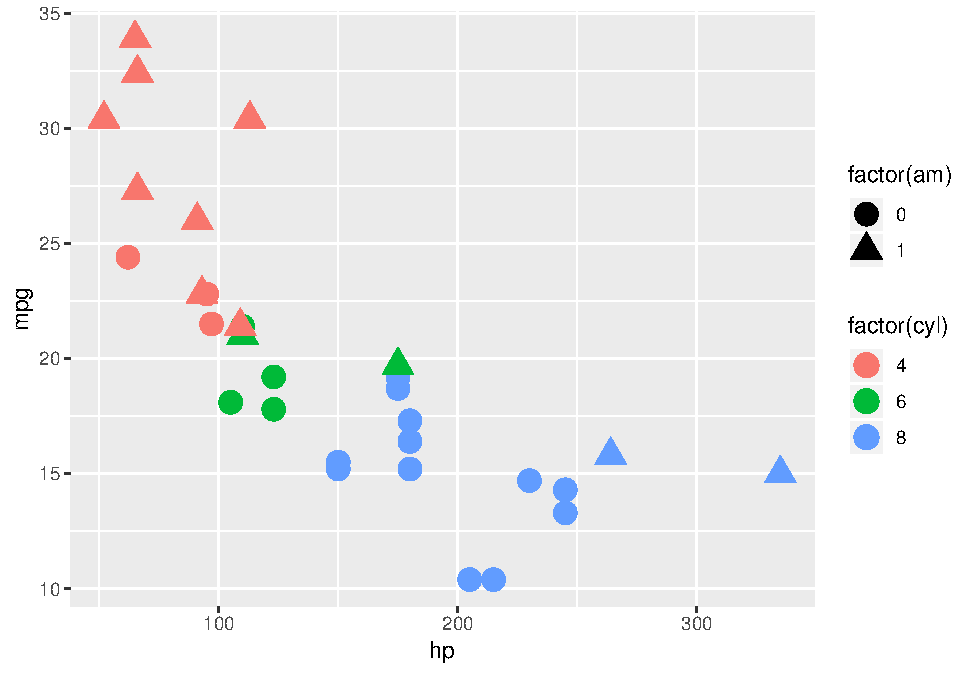
\includegraphics{stt-301-programming_files/figure-latex/unnamed-chunk-55-1.pdf}

\begin{Shaded}
\begin{Highlighting}[]
\KeywordTok{data}\NormalTok{(}\StringTok{"mtcars"}\NormalTok{)}
\KeywordTok{ggplot}\NormalTok{(}\DataTypeTok{data =}\NormalTok{ mtcars,}
       \DataTypeTok{mapping =} \KeywordTok{aes}\NormalTok{(}\DataTypeTok{x=}\NormalTok{hp, }\DataTypeTok{y=}\NormalTok{mpg)) }\OperatorTok{+}
\StringTok{  }\KeywordTok{geom_point}\NormalTok{(}\KeywordTok{aes}\NormalTok{(}\DataTypeTok{color =} \KeywordTok{factor}\NormalTok{(cyl),}
                 \DataTypeTok{shape =} \KeywordTok{factor}\NormalTok{(am)),}
             \DataTypeTok{size=}\DecValTok{5}\NormalTok{) }\OperatorTok{+}
\StringTok{  }\KeywordTok{facet_wrap}\NormalTok{(}\OperatorTok{~}\KeywordTok{factor}\NormalTok{(cyl))}
\end{Highlighting}
\end{Shaded}

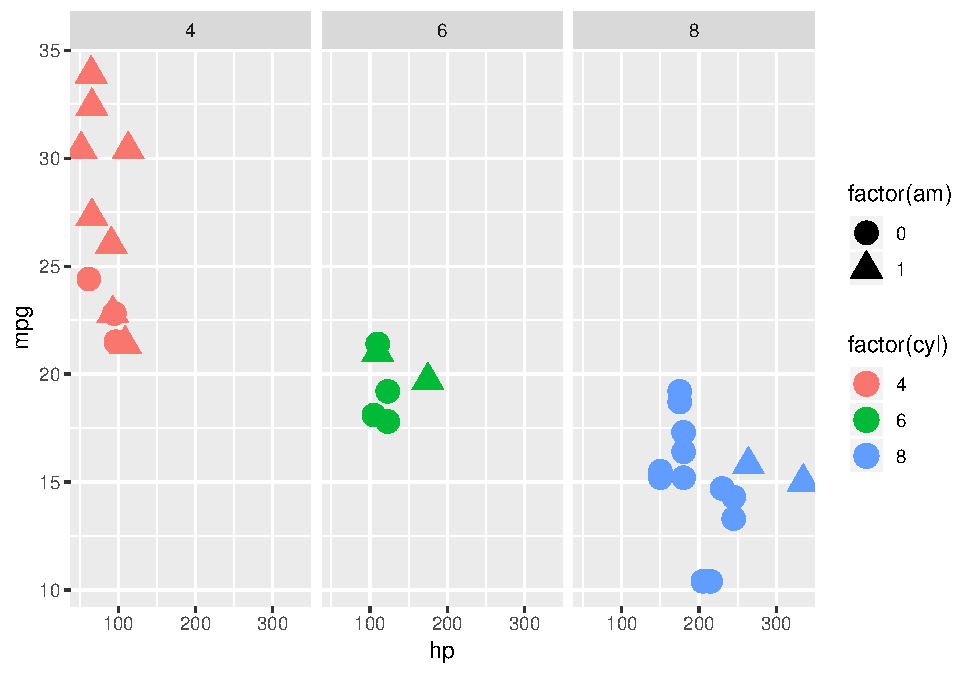
\includegraphics{stt-301-programming_files/figure-latex/unnamed-chunk-55-2.pdf}

\subsection{5.1 Scatter Plots}\label{scatter-plots}

Scatter plots are a workhorse of data visualization and provide a good
entry point to the ggplot2 system.

\begin{Shaded}
\begin{Highlighting}[]
\KeywordTok{data}\NormalTok{(iris)}
\KeywordTok{str}\NormalTok{(iris)}
\end{Highlighting}
\end{Shaded}

\begin{verbatim}
## 'data.frame':    150 obs. of  5 variables:
##  $ Sepal.Length: num  5.1 4.9 4.7 4.6 5 5.4 4.6 5 4.4 4.9 ...
##  $ Sepal.Width : num  3.5 3 3.2 3.1 3.6 3.9 3.4 3.4 2.9 3.1 ...
##  $ Petal.Length: num  1.4 1.4 1.3 1.5 1.4 1.7 1.4 1.5 1.4 1.5 ...
##  $ Petal.Width : num  0.2 0.2 0.2 0.2 0.2 0.4 0.3 0.2 0.2 0.1 ...
##  $ Species     : Factor w/ 3 levels "setosa","versicolor",..: 1 1 1 1 1 1 1 1 1 1 ...
\end{verbatim}

\begin{Shaded}
\begin{Highlighting}[]
\KeywordTok{library}\NormalTok{(ggplot2)}
\KeywordTok{ggplot}\NormalTok{(}\DataTypeTok{data =}\NormalTok{ iris, }\KeywordTok{aes}\NormalTok{(}\DataTypeTok{x =}\NormalTok{ Sepal.Length, }\DataTypeTok{y =}\NormalTok{ Sepal.Width)) }\OperatorTok{+}
\StringTok{       }\KeywordTok{geom_point}\NormalTok{()}
\end{Highlighting}
\end{Shaded}

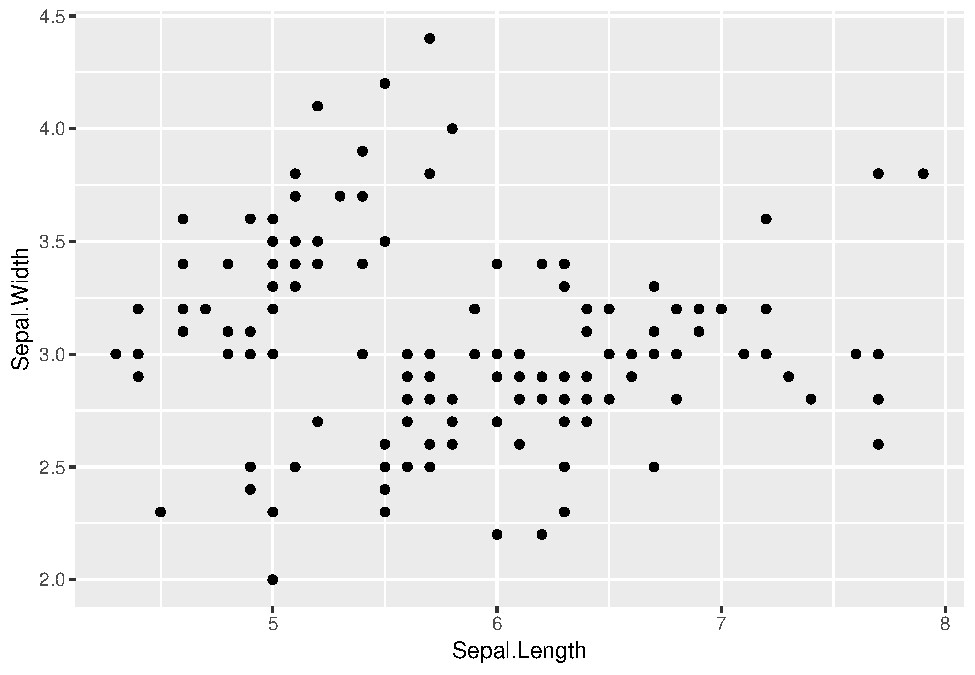
\includegraphics{stt-301-programming_files/figure-latex/unnamed-chunk-57-1.pdf}

\begin{Shaded}
\begin{Highlighting}[]
\KeywordTok{ggplot}\NormalTok{(}\DataTypeTok{data =}\NormalTok{ iris, }\KeywordTok{aes}\NormalTok{(}\DataTypeTok{x =}\NormalTok{ Sepal.Length, }\DataTypeTok{y =}\NormalTok{ Sepal.Width)) }\OperatorTok{+}
\StringTok{       }\KeywordTok{geom_point}\NormalTok{(}\DataTypeTok{size =} \DecValTok{4}\NormalTok{, }\KeywordTok{aes}\NormalTok{(}\DataTypeTok{color=}\NormalTok{Species, }\DataTypeTok{shape=}\NormalTok{Species))}
\end{Highlighting}
\end{Shaded}

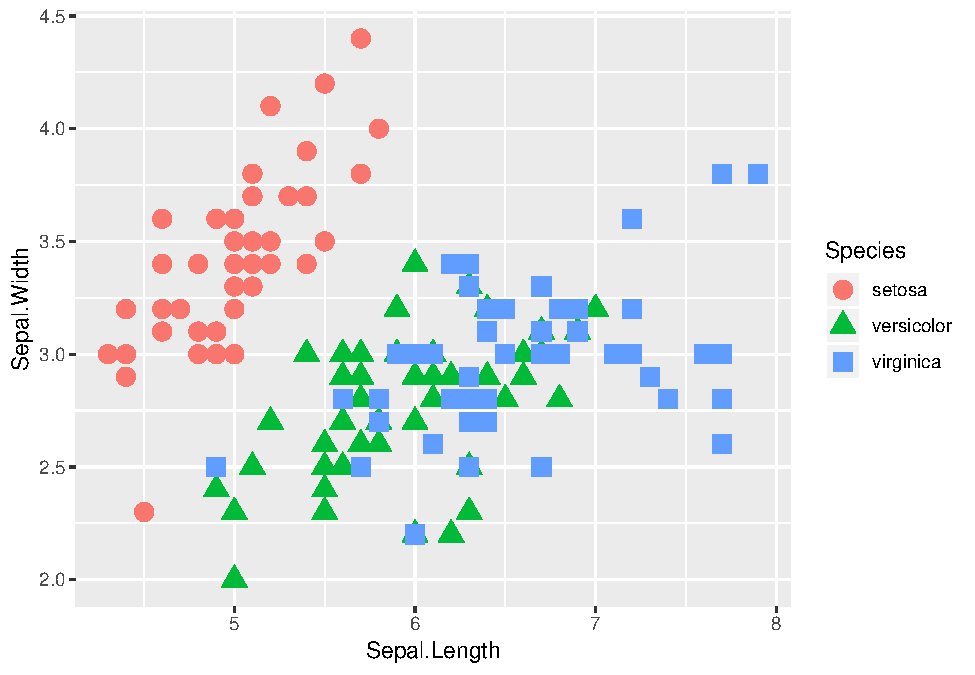
\includegraphics{stt-301-programming_files/figure-latex/unnamed-chunk-58-1.pdf}

\subsubsection{5.1.2 Adding lines to a scatter
plot}\label{adding-lines-to-a-scatter-plot}

\begin{Shaded}
\begin{Highlighting}[]
\KeywordTok{ggplot}\NormalTok{(}\DataTypeTok{data =}\NormalTok{ iris, }\KeywordTok{aes}\NormalTok{(}\DataTypeTok{x =}\NormalTok{ Sepal.Length, }\DataTypeTok{y =}\NormalTok{ Sepal.Width)) }\OperatorTok{+}
\StringTok{       }\KeywordTok{geom_point}\NormalTok{(}\DataTypeTok{size=}\DecValTok{3}\NormalTok{, }\KeywordTok{aes}\NormalTok{(}\DataTypeTok{color=}\NormalTok{Species)) }\OperatorTok{+}
\StringTok{       }\KeywordTok{stat_smooth}\NormalTok{(}\DataTypeTok{method =}\NormalTok{ lm, }\DataTypeTok{se=}\OtherTok{FALSE}\NormalTok{)}
\end{Highlighting}
\end{Shaded}

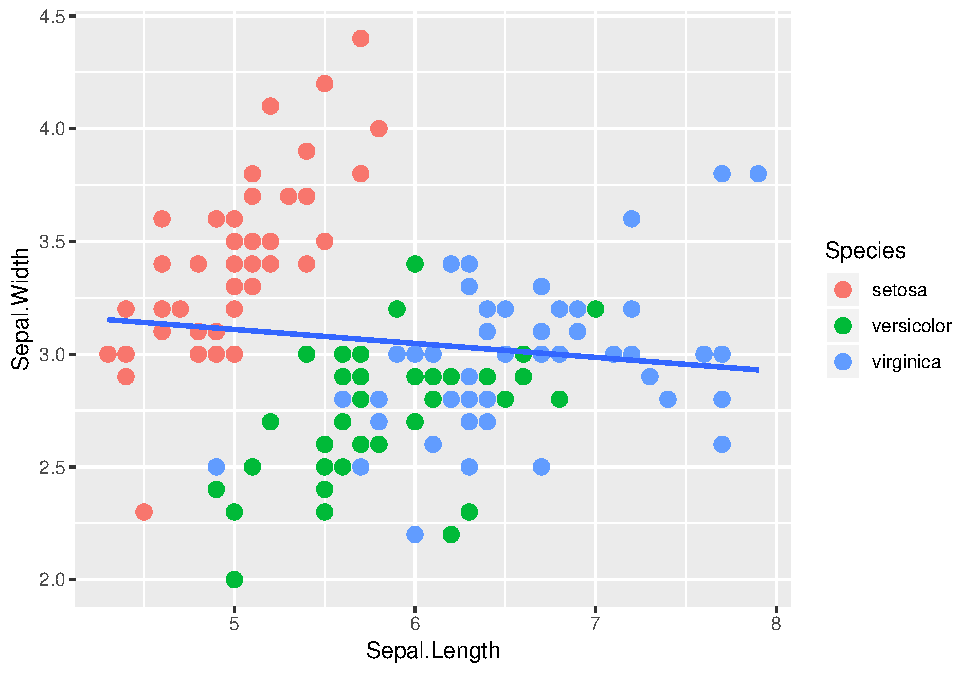
\includegraphics{stt-301-programming_files/figure-latex/unnamed-chunk-59-1.pdf}

For the iris data, it probably makes more sense to fit separate lines by
species. This can be specified using the aes() function inside
\texttt{stat\_smooth()}.

\begin{Shaded}
\begin{Highlighting}[]
\KeywordTok{ggplot}\NormalTok{(}\DataTypeTok{data =}\NormalTok{ iris, }\KeywordTok{aes}\NormalTok{(}\DataTypeTok{x =}\NormalTok{ Sepal.Length, }\DataTypeTok{y =}\NormalTok{ Sepal.Width)) }\OperatorTok{+}
\StringTok{      }\KeywordTok{geom_point}\NormalTok{(}\DataTypeTok{size=}\DecValTok{3}\NormalTok{, }\KeywordTok{aes}\NormalTok{(}\DataTypeTok{color=}\NormalTok{Species)) }\OperatorTok{+}
\StringTok{      }\KeywordTok{stat_smooth}\NormalTok{(}\DataTypeTok{method =}\NormalTok{ lm, }\DataTypeTok{se=}\OtherTok{FALSE}\NormalTok{, }\KeywordTok{aes}\NormalTok{(}\DataTypeTok{color=}\NormalTok{Species))}
\end{Highlighting}
\end{Shaded}

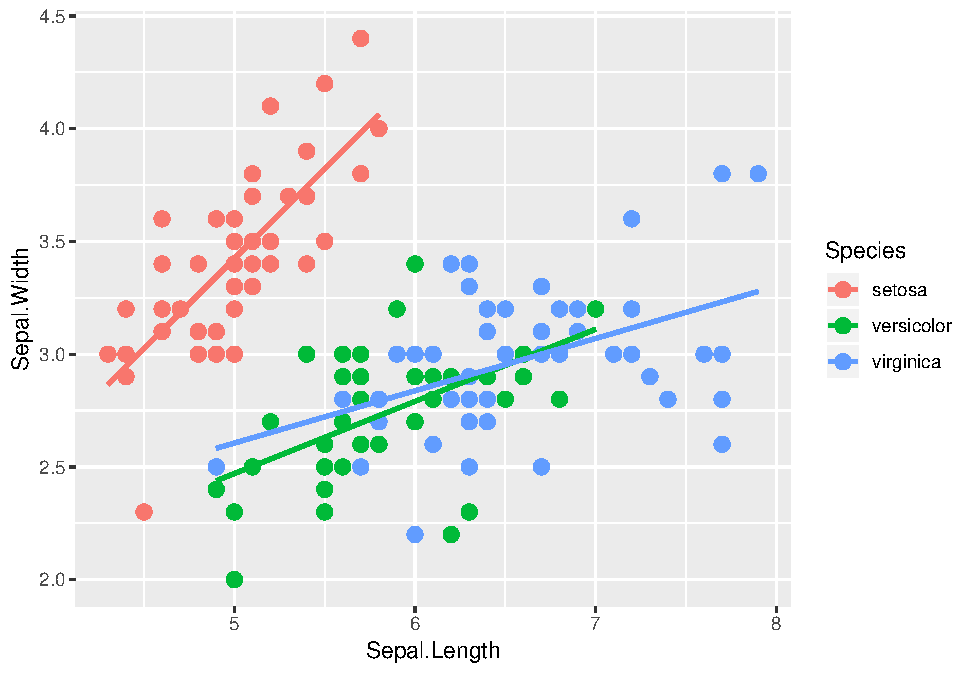
\includegraphics{stt-301-programming_files/figure-latex/unnamed-chunk-60-1.pdf}

Another common use of line segments in a graphic is to connect the
points in order, accomplished via the geom\_line() function.

\begin{Shaded}
\begin{Highlighting}[]
\KeywordTok{ggplot}\NormalTok{(}\DataTypeTok{data =}\NormalTok{ iris, }\KeywordTok{aes}\NormalTok{(}\DataTypeTok{x =}\NormalTok{ Sepal.Length, }\DataTypeTok{y =}\NormalTok{ Sepal.Width)) }\OperatorTok{+}
\StringTok{      }\KeywordTok{geom_point}\NormalTok{(}\DataTypeTok{size =} \DecValTok{4}\NormalTok{, }\KeywordTok{aes}\NormalTok{(}\DataTypeTok{color=}\NormalTok{Species, }\DataTypeTok{shape =}\NormalTok{ Species)) }\OperatorTok{+}
\StringTok{      }\KeywordTok{geom_line}\NormalTok{()}
\end{Highlighting}
\end{Shaded}

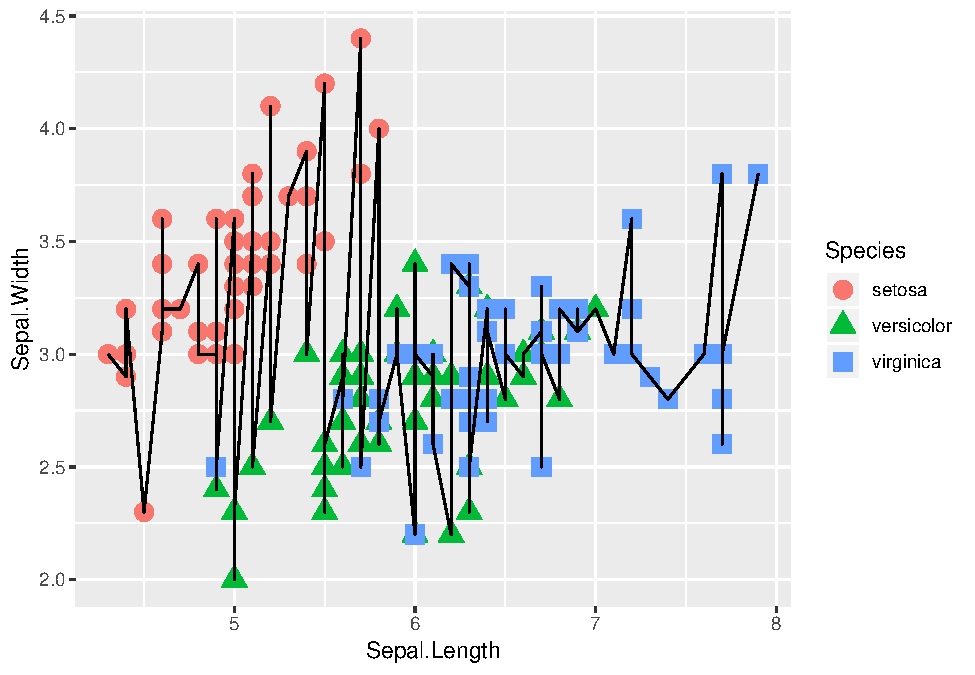
\includegraphics{stt-301-programming_files/figure-latex/unnamed-chunk-61-1.pdf}

\begin{Shaded}
\begin{Highlighting}[]
      \KeywordTok{ggplot}\NormalTok{(}\DataTypeTok{data =}\NormalTok{ iris, }\KeywordTok{aes}\NormalTok{(}\DataTypeTok{x =}\NormalTok{ Sepal.Length, }\DataTypeTok{y =}\NormalTok{ Sepal.Width)) }\OperatorTok{+}
\StringTok{      }\KeywordTok{geom_point}\NormalTok{(}\DataTypeTok{size =} \DecValTok{4}\NormalTok{, }\KeywordTok{aes}\NormalTok{(}\DataTypeTok{color=}\NormalTok{Species)) }\OperatorTok{+}
\StringTok{      }\KeywordTok{geom_line}\NormalTok{(}\KeywordTok{aes}\NormalTok{(}\DataTypeTok{color=}\NormalTok{Species))}
\end{Highlighting}
\end{Shaded}

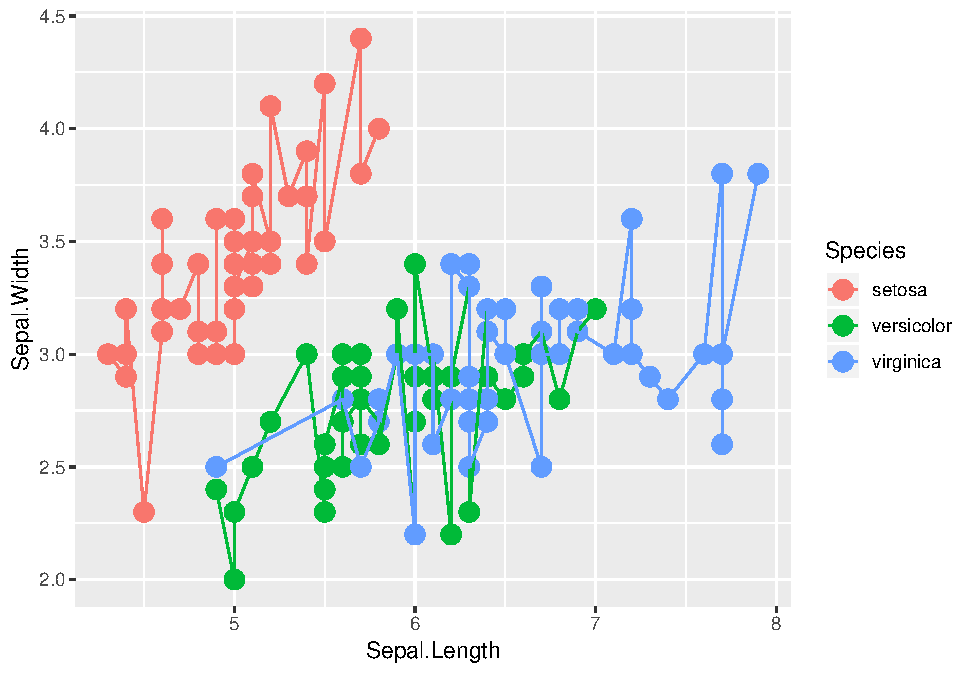
\includegraphics{stt-301-programming_files/figure-latex/unnamed-chunk-61-2.pdf}

\subsection{5.2.0 Labels, axes, text, etc.}\label{labels-axes-text-etc.}

\begin{Shaded}
\begin{Highlighting}[]
\NormalTok{u.crime <-}\StringTok{ "http://blue.for.msu.edu/FOR875/data/crimeRatesByState2005.csv"}
\NormalTok{crime <-}\StringTok{ }\KeywordTok{read.csv}\NormalTok{(u.crime, }\DataTypeTok{header=}\OtherTok{TRUE}\NormalTok{)}
\KeywordTok{str}\NormalTok{(crime)}
\end{Highlighting}
\end{Shaded}

\begin{verbatim}
## 'data.frame':    50 obs. of  9 variables:
##  $ state              : Factor w/ 50 levels "Alabama ","Alaska ",..: 1 2 3 4 5 6 7 8 9 10 ...
##  $ murder             : num  8.2 4.8 7.5 6.7 6.9 3.7 2.9 4.4 5 6.2 ...
##  $ Forcible_rate      : num  34.3 81.1 33.8 42.9 26 43.4 20 44.7 37.1 23.6 ...
##  $ Robbery            : num  141.4 80.9 144.4 91.1 176.1 ...
##  $ aggravated_assult  : num  248 465 327 387 317 ...
##  $ burglary           : num  954 622 948 1085 693 ...
##  $ larceny_theft      : num  2650 2599 2965 2711 1916 ...
##  $ motor_vehicle_theft: num  288 391 924 262 713 ...
##  $ population         : int  4627851 686293 6500180 2855390 36756666 4861515 3501252 873092 18328340 9685744 ...
\end{verbatim}

Here we use \texttt{labs()} to change the x and y axis labels and other
descriptive text.

\begin{Shaded}
\begin{Highlighting}[]
\KeywordTok{ggplot}\NormalTok{(}\DataTypeTok{data =}\NormalTok{ crime, }\KeywordTok{aes}\NormalTok{(}\DataTypeTok{x =}\NormalTok{ burglary, }\DataTypeTok{y =}\NormalTok{ motor_vehicle_theft)) }\OperatorTok{+}
\StringTok{  }\KeywordTok{geom_point}\NormalTok{() }\OperatorTok{+}
\StringTok{  }\KeywordTok{labs}\NormalTok{(}\DataTypeTok{x =} \StringTok{"Burglaries per 100,000 population"}\NormalTok{,}
       \DataTypeTok{y =} \StringTok{"Motor vehicle theft per 100,000 population"}\NormalTok{,}
       \DataTypeTok{title =} \StringTok{"Burglaries vs motor vehicle theft for US states"}\NormalTok{,}
       \DataTypeTok{subtitle =} \StringTok{"2005 crime rates and 2008 population"}\NormalTok{,}
       \DataTypeTok{caption =} \StringTok{"Data from Nathan Yau http://flowingdata.com"}
\NormalTok{)}
\end{Highlighting}
\end{Shaded}

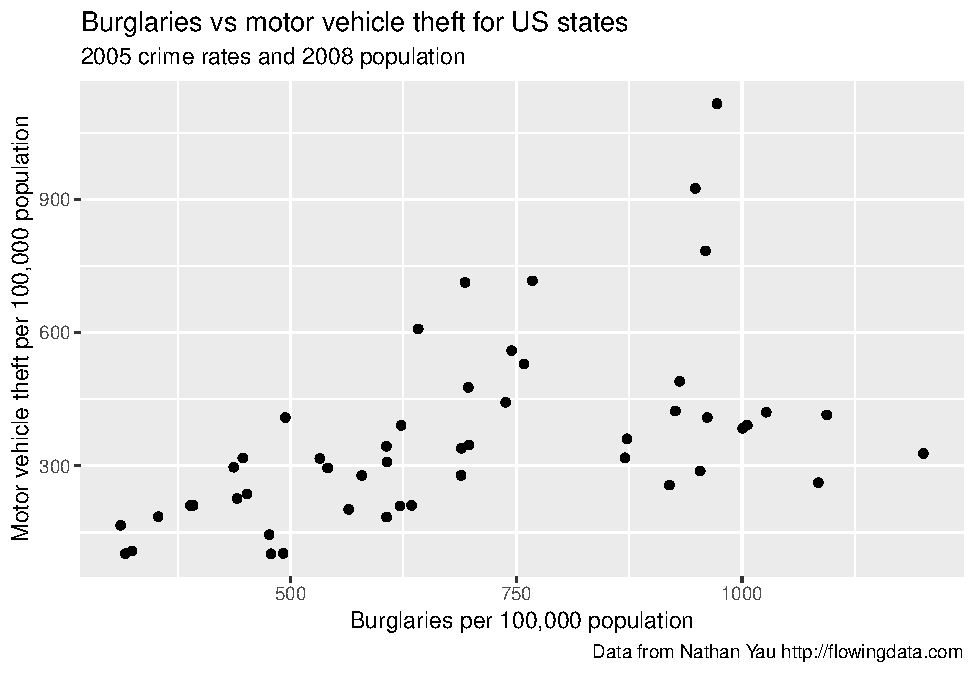
\includegraphics{stt-301-programming_files/figure-latex/unnamed-chunk-63-1.pdf}

\subsubsection{5.2.1 Customizing axes}\label{customizing-axes}

\texttt{ggplot} also provides default axis extents (i.e., limits) and
other axis features. These, and other axis features such as tick marks,
labels, and transformations, can be changed using the scale functions

\begin{Shaded}
\begin{Highlighting}[]
\KeywordTok{ggplot}\NormalTok{(}\DataTypeTok{data =}\NormalTok{ crime, }\KeywordTok{aes}\NormalTok{(}\DataTypeTok{x =}\NormalTok{ burglary, }\DataTypeTok{y =}\NormalTok{ motor_vehicle_theft)) }\OperatorTok{+}
\StringTok{  }\KeywordTok{geom_point}\NormalTok{() }\OperatorTok{+}
\StringTok{  }\KeywordTok{scale_x_continuous}\NormalTok{(}\DataTypeTok{name=}\StringTok{"Burglaries per 100,000 population"}\NormalTok{,}
                    \DataTypeTok{limits=}\KeywordTok{c}\NormalTok{(}\DecValTok{0}\NormalTok{,}\KeywordTok{max}\NormalTok{(crime}\OperatorTok{$}\NormalTok{burglary))) }\OperatorTok{+}
\StringTok{  }\KeywordTok{scale_y_continuous}\NormalTok{(}\DataTypeTok{name=}\StringTok{"Motor vehicle theft per 100,000 population"}\NormalTok{,}
                      \DataTypeTok{limits =} \KeywordTok{c}\NormalTok{(}\DecValTok{0}\NormalTok{, }\KeywordTok{max}\NormalTok{(crime}\OperatorTok{$}\NormalTok{motor_vehicle_theft)))}
\end{Highlighting}
\end{Shaded}

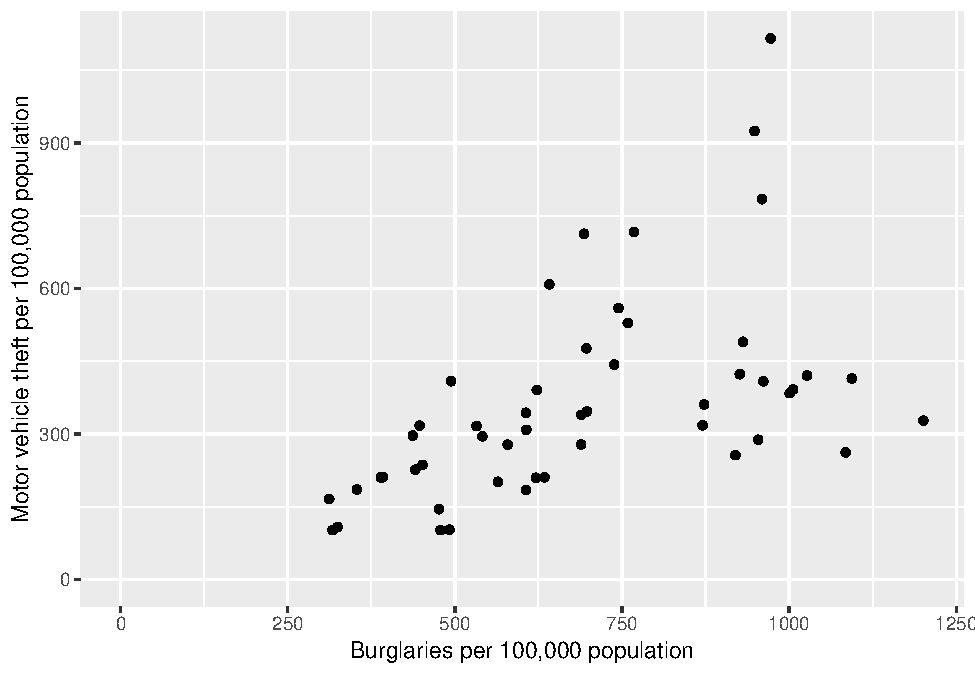
\includegraphics{stt-301-programming_files/figure-latex/unnamed-chunk-64-1.pdf}

\subsubsection{5.2.2 Text, point size, and
color}\label{text-point-size-and-color}

\begin{Shaded}
\begin{Highlighting}[]
\KeywordTok{ggplot}\NormalTok{(}\DataTypeTok{data =}\NormalTok{ crime, }\KeywordTok{aes}\NormalTok{(}\DataTypeTok{x =}\NormalTok{ burglary, }\DataTypeTok{y =}\NormalTok{ motor_vehicle_theft,}
       \DataTypeTok{size=}\NormalTok{population}\OperatorTok{/}\DecValTok{100000}\NormalTok{)) }\OperatorTok{+}
\StringTok{       }\KeywordTok{geom_point}\NormalTok{(}\DataTypeTok{color =} \StringTok{"blue"}\NormalTok{) }\OperatorTok{+}
\StringTok{       }\KeywordTok{geom_label}\NormalTok{(}\KeywordTok{aes}\NormalTok{(}\DataTypeTok{label =}\NormalTok{ state), }\DataTypeTok{alpha =} \FloatTok{0.5}\NormalTok{) }\OperatorTok{+}
\StringTok{       }\KeywordTok{scale_x_continuous}\NormalTok{(}\DataTypeTok{name=}\StringTok{"Burglaries per 100,000 population"}\NormalTok{,}
                     \DataTypeTok{limits=}\KeywordTok{c}\NormalTok{(}\DecValTok{0}\NormalTok{,}\KeywordTok{max}\NormalTok{(crime}\OperatorTok{$}\NormalTok{burglary))) }\OperatorTok{+}
\StringTok{        }\KeywordTok{scale_y_continuous}\NormalTok{(}\DataTypeTok{name=}\StringTok{"Motor vehicle theft per 100,000 population"}\NormalTok{,}
                     \DataTypeTok{limits =} \KeywordTok{c}\NormalTok{(}\DecValTok{0}\NormalTok{, }\KeywordTok{max}\NormalTok{(crime}\OperatorTok{$}\NormalTok{motor_vehicle_theft))) }\OperatorTok{+}
\StringTok{        }\KeywordTok{labs}\NormalTok{(}\DataTypeTok{size=}\StringTok{"Populationnn(100,000)"}\NormalTok{)}
\end{Highlighting}
\end{Shaded}

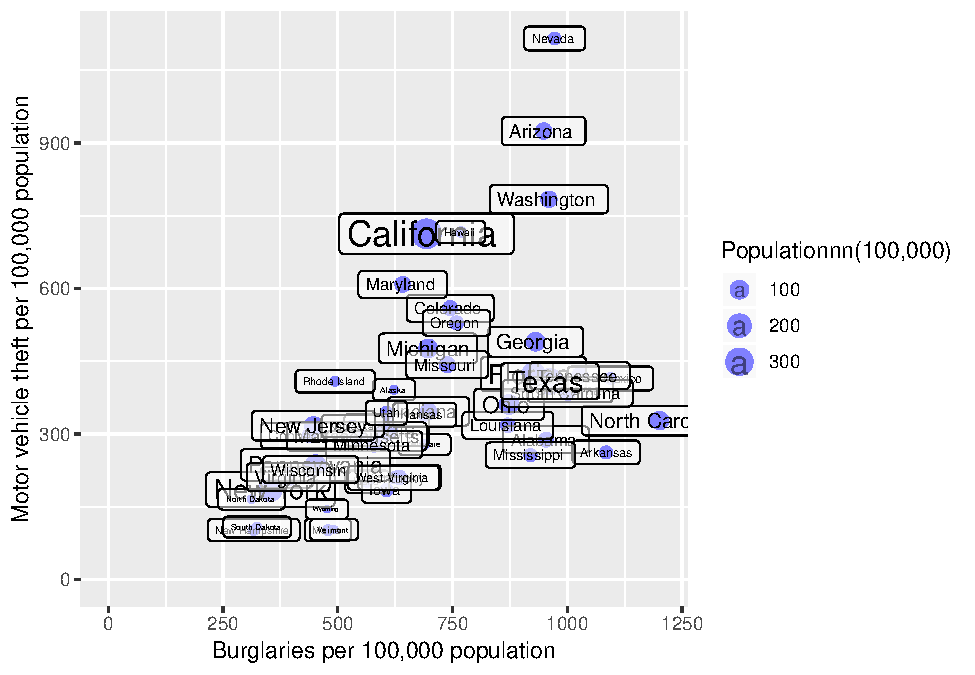
\includegraphics{stt-301-programming_files/figure-latex/unnamed-chunk-65-1.pdf}

\begin{Shaded}
\begin{Highlighting}[]
\KeywordTok{library}\NormalTok{(ggrepel)}
\KeywordTok{ggplot}\NormalTok{(}\DataTypeTok{data =}\NormalTok{ crime, }\KeywordTok{aes}\NormalTok{(}\DataTypeTok{x =}\NormalTok{ burglary, }\DataTypeTok{y =}\NormalTok{ motor_vehicle_theft,}
      \DataTypeTok{size=}\NormalTok{population}\OperatorTok{/}\DecValTok{100000}\NormalTok{)) }\OperatorTok{+}
\StringTok{      }\KeywordTok{geom_point}\NormalTok{(}\DataTypeTok{color =} \StringTok{"blue"}\NormalTok{) }\OperatorTok{+}
\StringTok{      }\KeywordTok{scale_x_continuous}\NormalTok{(}\DataTypeTok{name=}\StringTok{"Burglaries per 100,000 population"}\NormalTok{,}
                    \DataTypeTok{limits=}\KeywordTok{c}\NormalTok{(}\DecValTok{0}\NormalTok{,}\KeywordTok{max}\NormalTok{(crime}\OperatorTok{$}\NormalTok{burglary))) }\OperatorTok{+}
\StringTok{      }\KeywordTok{scale_y_continuous}\NormalTok{(}\DataTypeTok{name=}\StringTok{"Motor vehicle theft per 100,000 population"}\NormalTok{,}
                  \DataTypeTok{limits =} \KeywordTok{c}\NormalTok{(}\DecValTok{0}\NormalTok{, }\KeywordTok{max}\NormalTok{(crime}\OperatorTok{$}\NormalTok{motor_vehicle_theft))) }\OperatorTok{+}
\StringTok{      }\KeywordTok{labs}\NormalTok{(}\DataTypeTok{size=}\StringTok{"Populationnn(100,000)"}\NormalTok{) }\OperatorTok{+}
\StringTok{       }\NormalTok{ggrepel}\OperatorTok{::}\KeywordTok{geom_label_repel}\NormalTok{(}\KeywordTok{aes}\NormalTok{(}\DataTypeTok{label =}\NormalTok{ state), }\DataTypeTok{alpha =} \FloatTok{0.5}\NormalTok{)}
\end{Highlighting}
\end{Shaded}

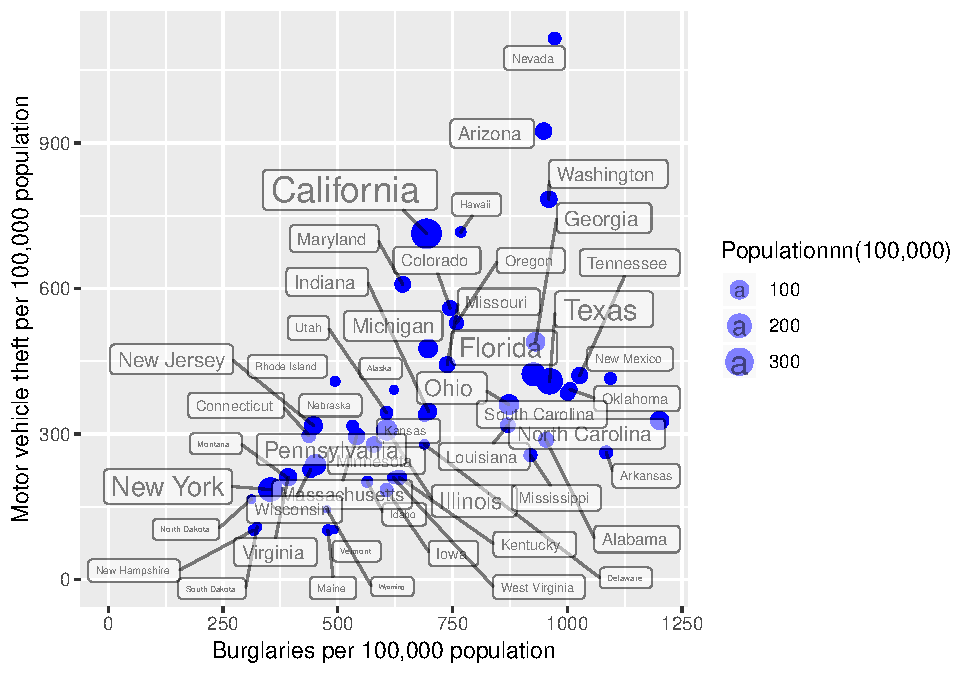
\includegraphics{stt-301-programming_files/figure-latex/unnamed-chunk-66-1.pdf}

geom\_raster: heatmap (x,y) geom\_density: density plot

\subsubsection{5.3.1 Histograms}\label{histograms}

Simon Newcomb conducted several experiments to estimate the speed of
light by measuring the time it took for light to travel from his
laboratory to a mirror at the base of the Washington Monument, and then
back to his lab.

\begin{Shaded}
\begin{Highlighting}[]
\NormalTok{u.newcomb <-}\StringTok{ "http://blue.for.msu.edu/FOR875/data/Newcomb.csv"}
\NormalTok{Newcomb <-}\StringTok{ }\KeywordTok{read.csv}\NormalTok{(u.newcomb, }\DataTypeTok{header =} \OtherTok{TRUE}\NormalTok{)}
\KeywordTok{head}\NormalTok{(Newcomb)}
\end{Highlighting}
\end{Shaded}

\begin{verbatim}
##   Time
## 1   28
## 2   26
## 3   33
## 4   24
## 5   34
## 6  -44
\end{verbatim}

\begin{Shaded}
\begin{Highlighting}[]
\KeywordTok{ggplot}\NormalTok{(Newcomb, }\KeywordTok{aes}\NormalTok{(}\DataTypeTok{x =}\NormalTok{ Time)) }\OperatorTok{+}\StringTok{ }\KeywordTok{geom_histogram}\NormalTok{()}
\end{Highlighting}
\end{Shaded}

\begin{verbatim}
## `stat_bin()` using `bins = 30`. Pick better value with `binwidth`.
\end{verbatim}

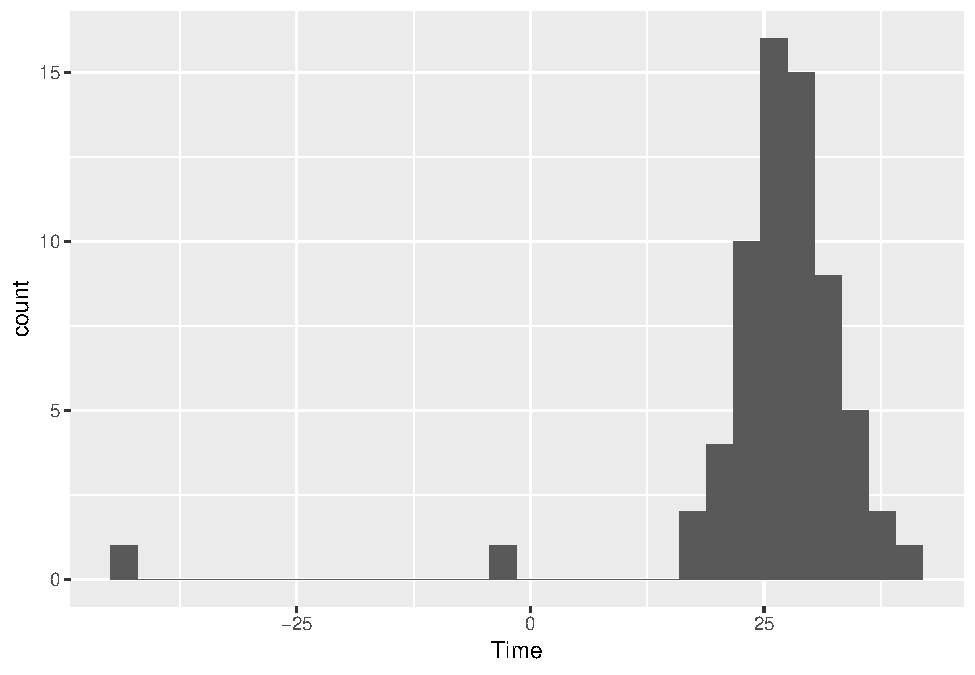
\includegraphics{stt-301-programming_files/figure-latex/unnamed-chunk-67-1.pdf}

\begin{Shaded}
\begin{Highlighting}[]
\KeywordTok{ggplot}\NormalTok{(Newcomb, }\KeywordTok{aes}\NormalTok{(}\DataTypeTok{x =}\NormalTok{ Time)) }\OperatorTok{+}
\KeywordTok{geom_histogram}\NormalTok{(}\DataTypeTok{binwidth =} \DecValTok{5}\NormalTok{, }\DataTypeTok{color =} \StringTok{"black"}\NormalTok{, }\DataTypeTok{fill =} \StringTok{"blue"}\NormalTok{ )}
\end{Highlighting}
\end{Shaded}

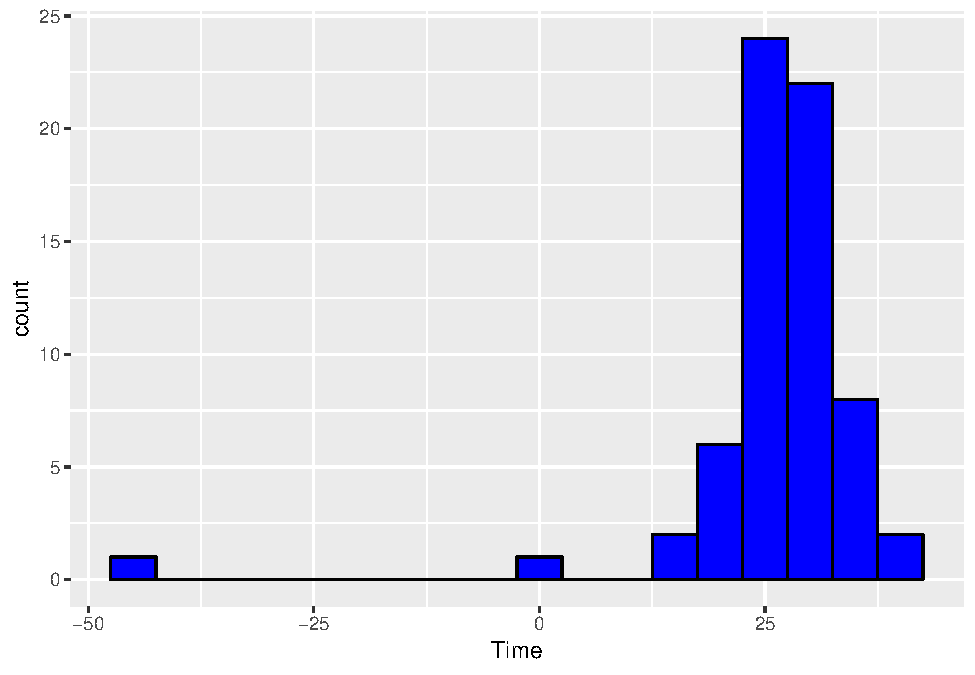
\includegraphics{stt-301-programming_files/figure-latex/unnamed-chunk-68-1.pdf}

\subsubsection{5.3.2 Boxplots}\label{boxplots}

\begin{Shaded}
\begin{Highlighting}[]
\KeywordTok{library}\NormalTok{(gapminder)}
\KeywordTok{ggplot}\NormalTok{(}\DataTypeTok{data =} \KeywordTok{subset}\NormalTok{(gapminder, year }\OperatorTok{==}\StringTok{ }\DecValTok{2002}\NormalTok{),}
     \KeywordTok{aes}\NormalTok{(}\DataTypeTok{x =}\NormalTok{ continent, }\DataTypeTok{y =}\NormalTok{ gdpPercap)) }\OperatorTok{+}
\StringTok{  }\KeywordTok{geom_boxplot}\NormalTok{(}\DataTypeTok{color =} \StringTok{"black"}\NormalTok{, }\DataTypeTok{fill =} \StringTok{"lightblue"}\NormalTok{)}
\end{Highlighting}
\end{Shaded}

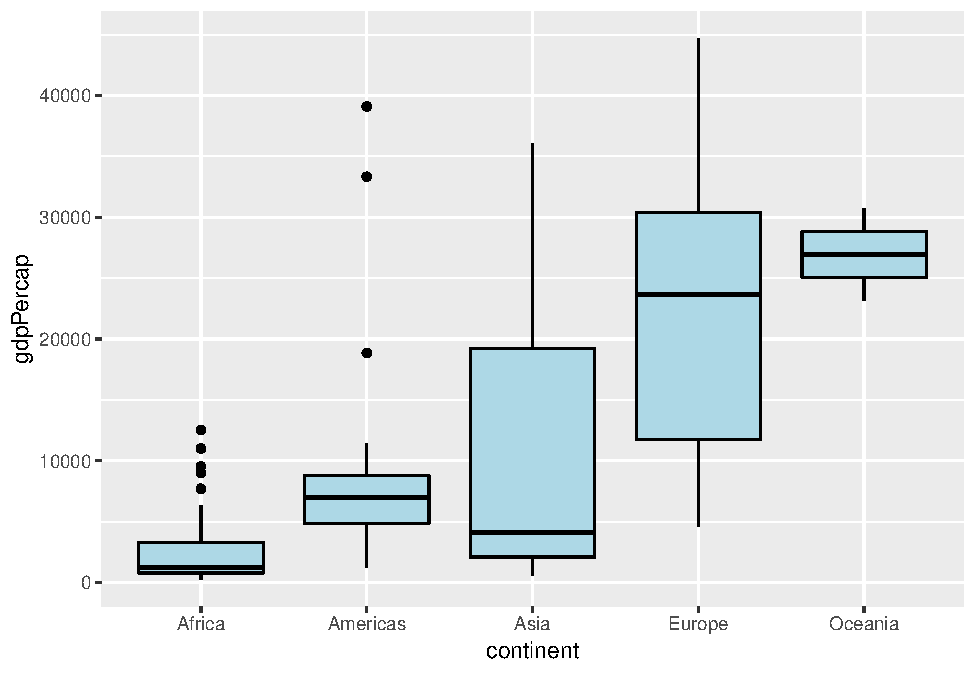
\includegraphics{stt-301-programming_files/figure-latex/unnamed-chunk-69-1.pdf}

\begin{Shaded}
\begin{Highlighting}[]
\KeywordTok{ggplot}\NormalTok{(}\DataTypeTok{data =} \KeywordTok{subset}\NormalTok{(gapminder, year }\OperatorTok{==}\StringTok{ }\DecValTok{2002}\NormalTok{),}
    \KeywordTok{aes}\NormalTok{(}\DataTypeTok{x =}\NormalTok{ continent, }\DataTypeTok{y =}\NormalTok{ gdpPercap)) }\OperatorTok{+}
\StringTok{  }\KeywordTok{geom_boxplot}\NormalTok{(}\DataTypeTok{color =} \StringTok{"red"}\NormalTok{, }\DataTypeTok{fill =} \StringTok{"lightblue"}\NormalTok{) }\OperatorTok{+}
\StringTok{  }\KeywordTok{scale_x_discrete}\NormalTok{(}\DataTypeTok{name =} \StringTok{"Continent"}\NormalTok{) }\OperatorTok{+}
\StringTok{  }\KeywordTok{scale_y_continuous}\NormalTok{(}\DataTypeTok{name =} \StringTok{"Per Capita GDP"}\NormalTok{) }\OperatorTok{+}\StringTok{ }\KeywordTok{coord_flip}\NormalTok{()}
\end{Highlighting}
\end{Shaded}

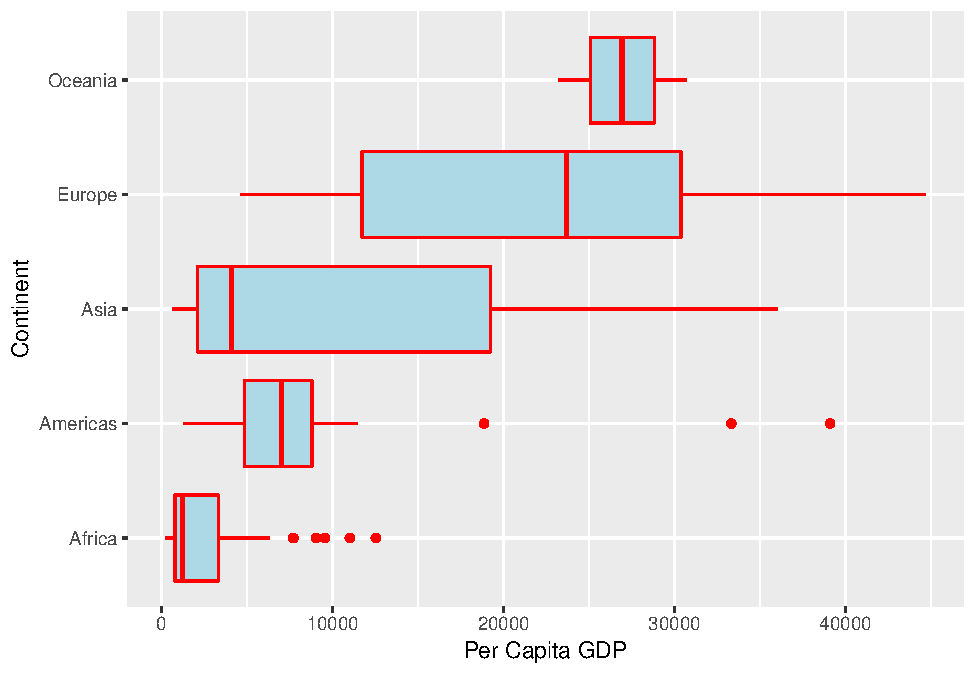
\includegraphics{stt-301-programming_files/figure-latex/unnamed-chunk-70-1.pdf}

\subsubsection{5.3.3 Bar graphs}\label{bar-graphs}

As part of a study, elementary school students were asked which was more
important to them: good grades, popularity, or athletic ability. Here is
a brief look at the data.

\begin{Shaded}
\begin{Highlighting}[]
\NormalTok{u.goals <-}\StringTok{ "http://blue.for.msu.edu/FOR875/data/StudentGoals.csv"}
\NormalTok{StudentGoals <-}\StringTok{ }\KeywordTok{read.csv}\NormalTok{(u.goals, }\DataTypeTok{header =} \OtherTok{TRUE}\NormalTok{)}
\KeywordTok{head}\NormalTok{(StudentGoals)}
\end{Highlighting}
\end{Shaded}

\begin{verbatim}
##   Gender Grade Age  Race  Type School   Goals Grades Sports Looks Money
## 1    boy     5  11 White Rural    Elm  Sports      1      2     4     3
## 2    boy     5  10 White Rural    Elm Popular      2      1     4     3
## 3   girl     5  11 White Rural    Elm Popular      4      3     1     2
## 4   girl     5  11 White Rural    Elm Popular      2      3     4     1
## 5   girl     5  10 White Rural    Elm Popular      4      2     1     3
## 6   girl     5  11 White Rural    Elm Popular      4      2     1     3
\end{verbatim}

First a simple bar graph of the most important goal chosen is drawn,
followed by a stacked bar graph which also includes the student's
gender, followed by a side by side bar graph which includes the
student's gender.

\begin{Shaded}
\begin{Highlighting}[]
\KeywordTok{ggplot}\NormalTok{(StudentGoals, }\KeywordTok{aes}\NormalTok{(}\DataTypeTok{x =}\NormalTok{ Goals)) }\OperatorTok{+}\StringTok{ }\KeywordTok{geom_bar}\NormalTok{()}
\end{Highlighting}
\end{Shaded}

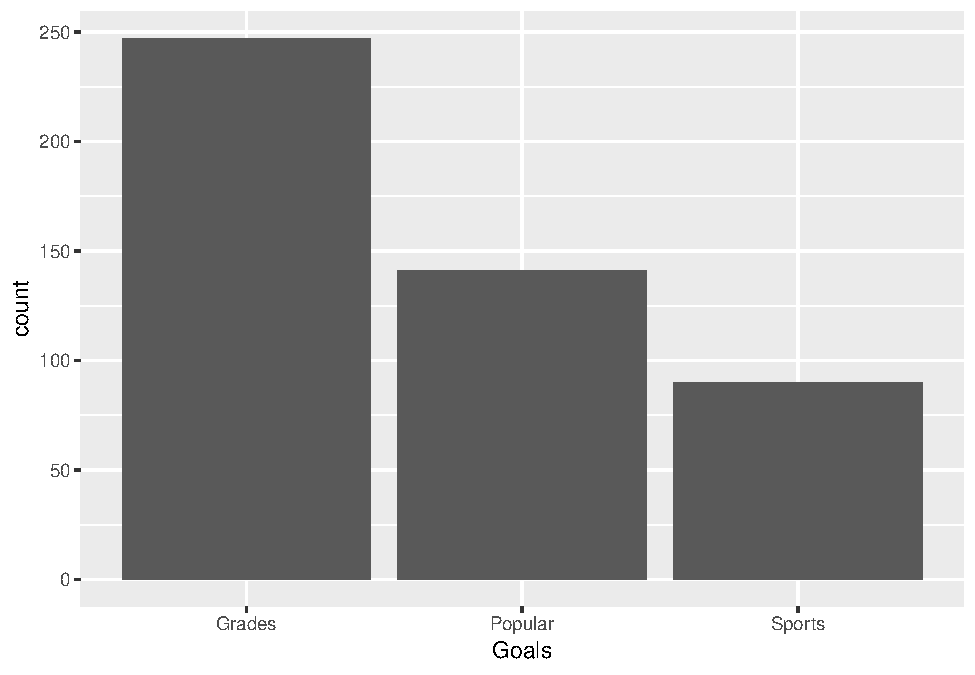
\includegraphics{stt-301-programming_files/figure-latex/unnamed-chunk-72-1.pdf}

\begin{Shaded}
\begin{Highlighting}[]
\KeywordTok{ggplot}\NormalTok{(StudentGoals, }\KeywordTok{aes}\NormalTok{(}\DataTypeTok{x =}\NormalTok{ Goals, }\DataTypeTok{fill =}\NormalTok{ Gender)) }\OperatorTok{+}\StringTok{ }\KeywordTok{geom_bar}\NormalTok{()}
\end{Highlighting}
\end{Shaded}

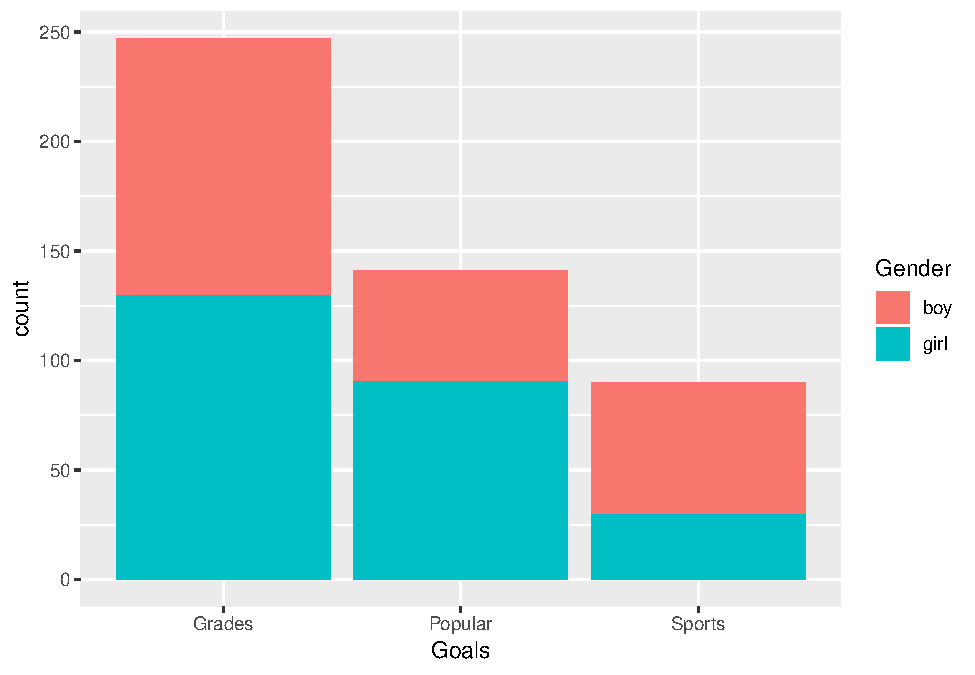
\includegraphics{stt-301-programming_files/figure-latex/unnamed-chunk-72-2.pdf}

\begin{Shaded}
\begin{Highlighting}[]
\KeywordTok{ggplot}\NormalTok{(StudentGoals, }\KeywordTok{aes}\NormalTok{(}\DataTypeTok{x =}\NormalTok{ Goals, }\DataTypeTok{fill =}\NormalTok{ Gender)) }\OperatorTok{+}
\StringTok{  }\KeywordTok{geom_bar}\NormalTok{(}\DataTypeTok{position =} \StringTok{"dodge"}\NormalTok{)}
\end{Highlighting}
\end{Shaded}

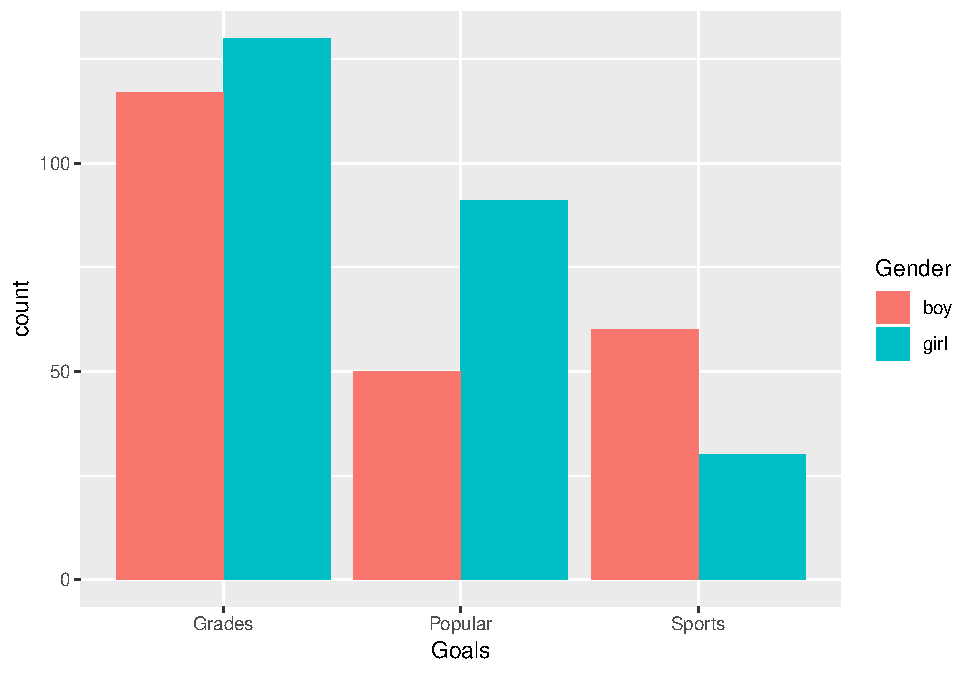
\includegraphics{stt-301-programming_files/figure-latex/unnamed-chunk-72-3.pdf}

In this example R counted the number of students who had each goal and
used these counts as the height of the bars. Sometimes the data contain
the bar heights as a variable. For example, we create a bar graph of
India's per capita GDP with separate bars for each year in the data

\begin{Shaded}
\begin{Highlighting}[]
\KeywordTok{ggplot}\NormalTok{(}\KeywordTok{subset}\NormalTok{(gapminder, country }\OperatorTok{==}\StringTok{ "India"}\NormalTok{), }\KeywordTok{aes}\NormalTok{(}\DataTypeTok{x =}\NormalTok{ year, }\DataTypeTok{y =}\NormalTok{ gdpPercap)) }\OperatorTok{+}
\StringTok{  }\KeywordTok{geom_bar}\NormalTok{(}\DataTypeTok{stat =} \StringTok{"identity"}\NormalTok{, }\DataTypeTok{color =} \StringTok{"black"}\NormalTok{, }\DataTypeTok{fill =} \StringTok{"steelblue2"}\NormalTok{) }\OperatorTok{+}
\StringTok{  }\KeywordTok{ggtitle}\NormalTok{(}\StringTok{"India's per-capita GDP"}\NormalTok{)}
\end{Highlighting}
\end{Shaded}

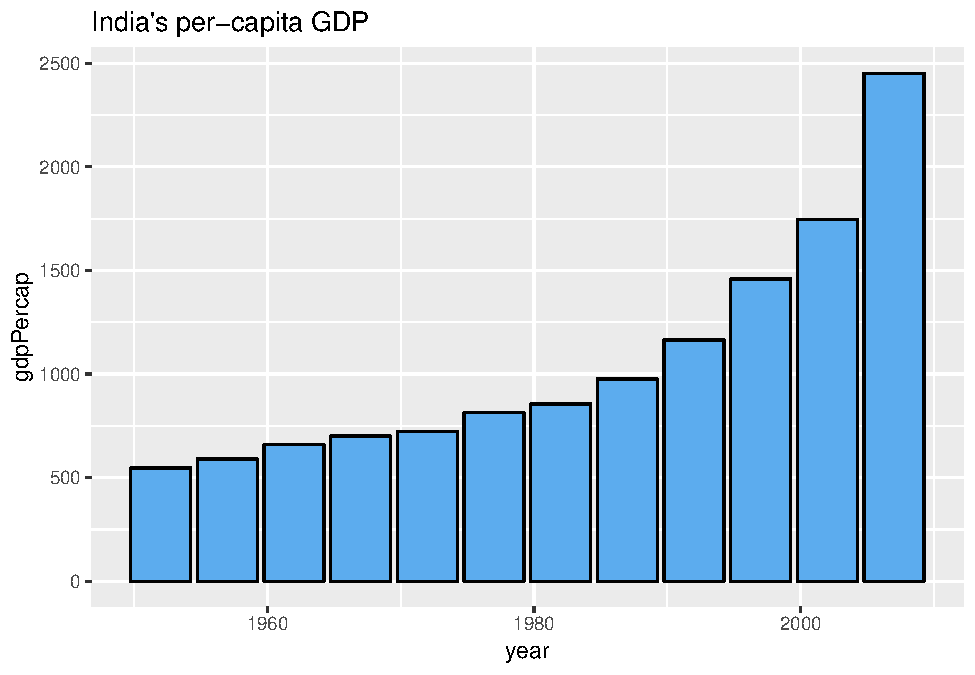
\includegraphics{stt-301-programming_files/figure-latex/unnamed-chunk-73-1.pdf}

\subsubsection{5.3.4 Graphs of functions}\label{graphs-of-functions}

\begin{Shaded}
\begin{Highlighting}[]
\NormalTok{x <-}\StringTok{ }\KeywordTok{seq}\NormalTok{(}\OperatorTok{-}\NormalTok{pi, pi, }\DataTypeTok{len =} \DecValTok{1000}\NormalTok{)}
\NormalTok{sin.data <-}\StringTok{ }\KeywordTok{data.frame}\NormalTok{(}\DataTypeTok{x =}\NormalTok{ x, }\DataTypeTok{y =} \KeywordTok{sin}\NormalTok{(x))}
\KeywordTok{ggplot}\NormalTok{(}\DataTypeTok{data =}\NormalTok{ sin.data, }\KeywordTok{aes}\NormalTok{(}\DataTypeTok{x =}\NormalTok{ x, }\DataTypeTok{y =}\NormalTok{ y)) }\OperatorTok{+}\StringTok{ }\KeywordTok{geom_line}\NormalTok{() }\OperatorTok{+}
\StringTok{  }\KeywordTok{scale_y_continuous}\NormalTok{(}\DataTypeTok{name =} \StringTok{"sin(x)"}\NormalTok{)}
\end{Highlighting}
\end{Shaded}

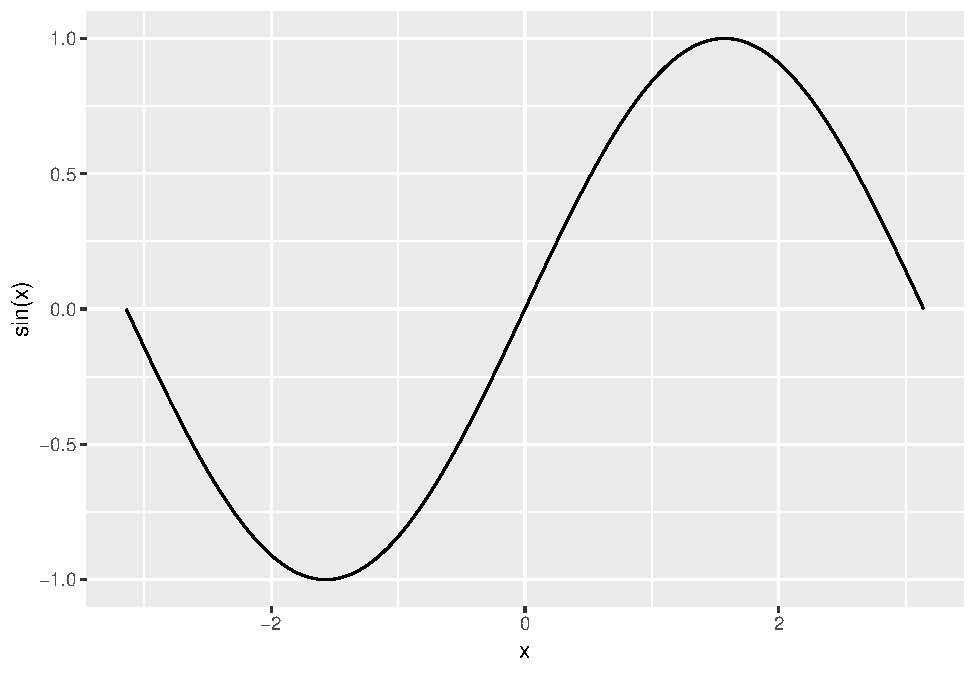
\includegraphics{stt-301-programming_files/figure-latex/unnamed-chunk-74-1.pdf}

\subsection{5.4 Themes}\label{themes}

Default themes include: \texttt{theme\_bw()}, \texttt{theme\_classic()},
\texttt{theme\_dark()}, \texttt{theme\_gray()}, \texttt{theme\_light()},
\texttt{theme\_linedraw()}, \texttt{theme\_minimal()}, and
\texttt{theme\_void()}.

\begin{Shaded}
\begin{Highlighting}[]
\KeywordTok{ggplot}\NormalTok{(}\DataTypeTok{data =}\NormalTok{ sin.data, }\KeywordTok{aes}\NormalTok{(}\DataTypeTok{x =}\NormalTok{ x, }\DataTypeTok{y =}\NormalTok{ y)) }\OperatorTok{+}\StringTok{ }\KeywordTok{geom_line}\NormalTok{() }\OperatorTok{+}
\StringTok{  }\KeywordTok{scale_y_continuous}\NormalTok{(}\DataTypeTok{name =} \StringTok{"sin(x)"}\NormalTok{) }\OperatorTok{+}
\StringTok{  }\KeywordTok{theme_classic}\NormalTok{()}
\end{Highlighting}
\end{Shaded}

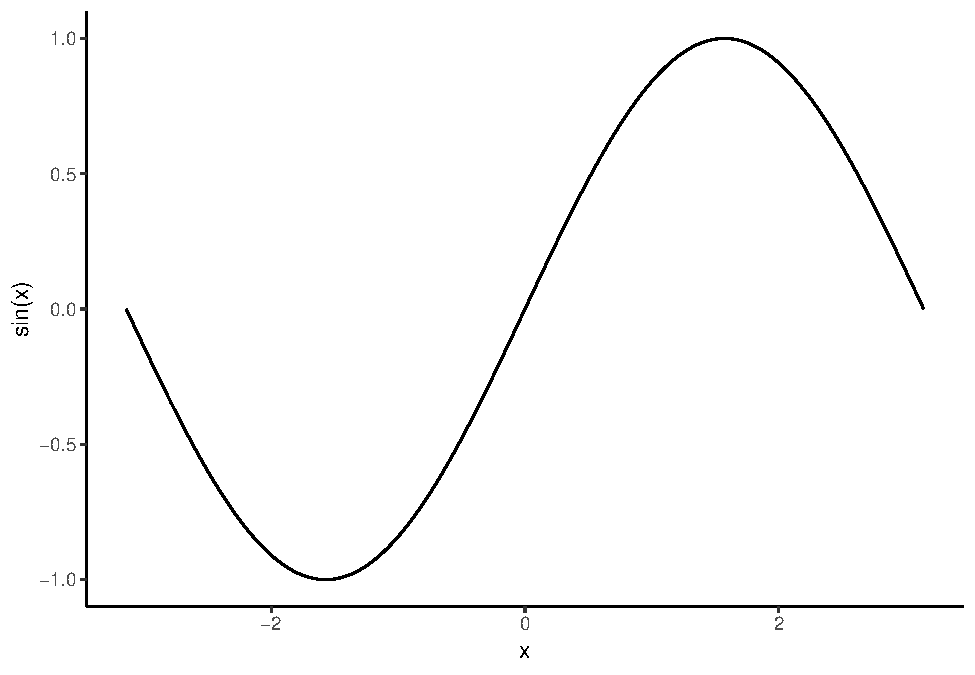
\includegraphics{stt-301-programming_files/figure-latex/unnamed-chunk-75-1.pdf}

The ggthemes add-on package \url{https://github.com/jrnold/ggthemes} by
Jefrey Arnold provides a large selection of themes beyond the eight
themes that come with ggplot2

\subsection{5.5 Saving graphics}\label{saving-graphics}

formats. The \texttt{ggsave()} function will allow you to save your most
recent \texttt{ggplot()} to a variety of vector (e.g., ``eps'', ``ps'',
``pdf'', ``svg'') or raster (e.g., ``jpeg'', ``tif'', ``png'', ``bmp'',
``wmf'') formats. The subsequent call to \texttt{ggsave()} saves
the\texttt{sin.data\ plot} to a pdf file called ``sin-plot.pdf''.

\begin{Shaded}
\begin{Highlighting}[]
\KeywordTok{ggplot}\NormalTok{(}\DataTypeTok{filename =} \StringTok{"sin-plot.pdf"}\NormalTok{, }\DataTypeTok{device=}\StringTok{"pdf"}\NormalTok{)}
\end{Highlighting}
\end{Shaded}


\includegraphics{stt-301-programming_files/figure-latex/unnamed-chunk-76-1.pdf}

\section{Working with Data}\label{working-with-data}

This involves bringing data into R, exporting data from R in a form that
is readable by other software, cleaning and reshaping data, and other
data manipulation

\subsection{6.1 Reading data into R}\label{reading-data-into-r}

Data come in a dizzying variety of forms. It might be in a proprietary
format such as an .xlsx Excel file, a .sav SPSS file, or a .mtw Minitab
file.

The \texttt{read.table()} function is used to read these data into an R
data frame.

\begin{Shaded}
\begin{Highlighting}[]
\NormalTok{u.bb <-}\StringTok{ "http://blue.for.msu.edu/FOR875/data/BrainAndBody.csv"}
\NormalTok{BrainBody <-}\StringTok{ }\KeywordTok{read.table}\NormalTok{(}\DataTypeTok{file =}\NormalTok{ u.bb, }\DataTypeTok{header =} \OtherTok{TRUE}\NormalTok{, }\DataTypeTok{sep =} \StringTok{","}\NormalTok{,}
\DataTypeTok{stringsAsFactors =} \OtherTok{FALSE}\NormalTok{)}
\KeywordTok{head}\NormalTok{(BrainBody)}
\end{Highlighting}
\end{Shaded}

\begin{verbatim}
##       body brain            name
## 1     1.35   8.1 Mountain beaver
## 2   465.00 423.0             Cow
## 3    36.33 119.5       Grey wolf
## 4    27.66 115.0            Goat
## 5     1.04   5.5      Guinea pig
## 6 11700.00  50.0     Dipliodocus
\end{verbatim}

The arguments used in this call to \texttt{read.table()} include:

\begin{enumerate}
\def\labelenumi{\arabic{enumi}.}
\tightlist
\item
  \texttt{file\ =\ u.bb}, which tells R the location of the file.
\item
  \texttt{header\ =\ TRUE}, which tells R the first line of the file
  gives the names of the variables.
\item
  \texttt{sep\ =\ ","}, which tells R that a comma separates the fields
  in the file.
\item
  \texttt{stringsAsFactors\ =\ FALSE} which tells R not to convert
  character vectors to factors.
\end{enumerate}

The function \texttt{read.csv()} is the same as read.table() except the
default separator is a comma, whereas the default separator for
\texttt{read.table()} is whitespace.

The file
\href{http://blue.for.msu.edu/FOR875/data/BrainAndBody.tsv}{BrainAndBody.tsv}
contains the same data, except a tab is used in place of a comma to
separate fields.

\begin{Shaded}
\begin{Highlighting}[]
\NormalTok{u.bb <-}\StringTok{ "http://blue.for.msu.edu/FOR875/data/BrainAndBody.tsv"}
\NormalTok{BrainBody <-}\StringTok{ }\KeywordTok{read.table}\NormalTok{(}\DataTypeTok{file =}\NormalTok{ u.bb, }\DataTypeTok{header =} \OtherTok{TRUE}\NormalTok{, }\DataTypeTok{sep =} \StringTok{"}\CharTok{\textbackslash{}t}\StringTok{"}\NormalTok{,}
\DataTypeTok{stringsAsFactors =} \OtherTok{FALSE}\NormalTok{)}
\KeywordTok{head}\NormalTok{(BrainBody)}
\end{Highlighting}
\end{Shaded}

\begin{verbatim}
##       body brain            name
## 1     1.35   8.1 Mountain beaver
## 2   465.00 423.0             Cow
## 3    36.33 119.5       Grey wolf
## 4    27.66 115.0            Goat
## 5     1.04   5.5      Guinea pig
## 6 11700.00  50.0     Dipliodocus
\end{verbatim}

A third file,
\href{\%22http://blue.for.msu.edu/FOR875/data/BrainAndBody.txt\%22}{BrainAndBody.txt},
contains the same data, but also contains a fewnlines of explanatory
text above the names of the variables. It also uses whitespacen rather
than a comma or a tab as a separator.

\begin{Shaded}
\begin{Highlighting}[]
\NormalTok{u.bb <-}\StringTok{ "http://blue.for.msu.edu/FOR875/data/BrainAndBody.txt"}
\NormalTok{BrainBody3 <-}\StringTok{ }\KeywordTok{read.table}\NormalTok{(u.bb, }\DataTypeTok{header =} \OtherTok{TRUE}\NormalTok{, }\DataTypeTok{sep =} \StringTok{" "}\NormalTok{, }\DataTypeTok{stringsAsFactors =} \OtherTok{FALSE}\NormalTok{, }\DataTypeTok{skip =} \DecValTok{4}\NormalTok{)}
\NormalTok{BrainBody3[}\DecValTok{1}\OperatorTok{:}\DecValTok{10}\NormalTok{,]}
\end{Highlighting}
\end{Shaded}

\begin{verbatim}
##        body  brain            name
## 1      1.35    8.1 Mountain beaver
## 2    465.00  423.0             Cow
## 3     36.33  119.5       Grey wolf
## 4     27.66  115.0            Goat
## 5      1.04    5.5      Guinea pig
## 6  11700.00   50.0     Dipliodocus
## 7   2547.00 4603.0  Asian elephant
## 8    187.10  419.0          Donkey
## 9    521.00  655.0           Horse
## 10    10.00  115.0    Potar monkey
\end{verbatim}

\subsubsection{6.1.1 Reading data with missing
observations}\label{reading-data-with-missing-observations}

The read.table() function has an argument \texttt{na.string} which
allows the user to specify how missing data is indicated in the source
file.

Argument \texttt{na.string\ =\ ""} which tells R the file indicates
missing data by leaving the appropriate entry blank.

\begin{Shaded}
\begin{Highlighting}[]
\NormalTok{u.weather <-}\StringTok{ "http://blue.for.msu.edu/FOR875/data/WeatherKLAN2014.csv"}
\NormalTok{WeatherKLAN2014 <-}\StringTok{ }\KeywordTok{read.csv}\NormalTok{(u.weather, }\DataTypeTok{header=}\OtherTok{TRUE}\NormalTok{, }\DataTypeTok{stringsAsFactors =} \OtherTok{FALSE}\NormalTok{, }\DataTypeTok{na.string =} \StringTok{""}\NormalTok{)}

\NormalTok{WeatherKLAN2014[}\DecValTok{1}\OperatorTok{:}\DecValTok{15}\NormalTok{,]}
\end{Highlighting}
\end{Shaded}

\begin{verbatim}
##        EST Max.TemperatureF Min.TemperatureF        Events
## 1   1/1/14               14                9          Snow
## 2   1/2/14               13               -3          Snow
## 3   1/3/14               13              -11          Snow
## 4   1/4/14               31               13          Snow
## 5   1/5/14               29               16      Fog-Snow
## 6   1/6/14               16              -12      Fog-Snow
## 7   1/7/14                2              -13          Snow
## 8   1/8/14               17               -1          Snow
## 9   1/9/14               21                2          Snow
## 10 1/10/14               39               21 Fog-Rain-Snow
## 11 1/11/14               41               32      Fog-Rain
## 12 1/12/14               39               31          <NA>
## 13 1/13/14               44               34          Rain
## 14 1/14/14               37               26     Rain-Snow
## 15 1/15/14               27               18          Snow
\end{verbatim}

\subsection{6.2 Summarizing data frames}\label{summarizing-data-frames}

Some common data tasks include variable summaries such as means or
standard deviations, transforming an existing variable, and creating new
variables.

\subsubsection{6.2.1 Column (and row)
summaries}\label{column-and-row-summaries}

\begin{Shaded}
\begin{Highlighting}[]
\NormalTok{u.weather <-}\StringTok{ "http://blue.for.msu.edu/FOR875/data/WeatherKLAN2014Full.csv"}
\NormalTok{WeatherKLAN2014Full <-}\StringTok{ }\KeywordTok{read.csv}\NormalTok{(u.weather, }\DataTypeTok{header=}\OtherTok{TRUE}\NormalTok{, }\DataTypeTok{stringsAsFactors =} \OtherTok{FALSE}\NormalTok{, }\DataTypeTok{na.string =} \StringTok{""}\NormalTok{)}
\KeywordTok{names}\NormalTok{(WeatherKLAN2014Full)}
\end{Highlighting}
\end{Shaded}

\begin{verbatim}
##  [1] "EST"                       "Max.TemperatureF"         
##  [3] "Mean.TemperatureF"         "Min.TemperatureF"         
##  [5] "Max.Dew.PointF"            "MeanDew.PointF"           
##  [7] "Min.DewpointF"             "Max.Humidity"             
##  [9] "Mean.Humidity"             "Min.Humidity"             
## [11] "Max.Sea.Level.PressureIn"  "Mean.Sea.Level.PressureIn"
## [13] "Min.Sea.Level.PressureIn"  "Max.VisibilityMiles"      
## [15] "Mean.VisibilityMiles"      "Min.VisibilityMiles"      
## [17] "Max.Wind.SpeedMPH"         "Mean.Wind.SpeedMPH"       
## [19] "Max.Gust.SpeedMPH"         "PrecipitationIn"          
## [21] "CloudCover"                "Events"                   
## [23] "WindDirDegrees"
\end{verbatim}

\paragraph{6.2.1.1 Mean}\label{mean}

To compute \texttt{mean()} for each column we can:

\begin{Shaded}
\begin{Highlighting}[]
\KeywordTok{mean}\NormalTok{(WeatherKLAN2014Full}\OperatorTok{$}\NormalTok{Mean.TemperatureF)}
\end{Highlighting}
\end{Shaded}

\begin{verbatim}
## [1] 45.78082
\end{verbatim}

\begin{Shaded}
\begin{Highlighting}[]
\KeywordTok{mean}\NormalTok{(WeatherKLAN2014Full}\OperatorTok{$}\NormalTok{Min.TemperatureF)}
\end{Highlighting}
\end{Shaded}

\begin{verbatim}
## [1] 36.25479
\end{verbatim}

\begin{Shaded}
\begin{Highlighting}[]
\KeywordTok{mean}\NormalTok{(WeatherKLAN2014Full}\OperatorTok{$}\NormalTok{Max.TemperatureF)}
\end{Highlighting}
\end{Shaded}

\begin{verbatim}
## [1] 54.83836
\end{verbatim}

\begin{Shaded}
\begin{Highlighting}[]
\NormalTok{## Et Cetera}
\end{Highlighting}
\end{Shaded}

However, this wastes a lot of time. We can save time by using
\texttt{colMeans()} function which computes the mean of each (or
specified) columns in a data frame.

\begin{Shaded}
\begin{Highlighting}[]
\KeywordTok{colMeans}\NormalTok{(WeatherKLAN2014Full[, }\KeywordTok{c}\NormalTok{(}\DecValTok{2}\OperatorTok{:}\DecValTok{19}\NormalTok{, }\DecValTok{21}\NormalTok{, }\DecValTok{23}\NormalTok{)])}
\end{Highlighting}
\end{Shaded}

\begin{verbatim}
##          Max.TemperatureF         Mean.TemperatureF 
##                 54.838356                 45.780822 
##          Min.TemperatureF            Max.Dew.PointF 
##                 36.254795                 41.800000 
##            MeanDew.PointF             Min.DewpointF 
##                 36.394521                 30.156164 
##              Max.Humidity             Mean.Humidity 
##                 88.082192                 70.391781 
##              Min.Humidity  Max.Sea.Level.PressureIn 
##                 52.200000                 30.130247 
## Mean.Sea.Level.PressureIn  Min.Sea.Level.PressureIn 
##                 30.015370                 29.903890 
##       Max.VisibilityMiles      Mean.VisibilityMiles 
##                  9.895890                  8.249315 
##       Min.VisibilityMiles         Max.Wind.SpeedMPH 
##                  4.824658                 19.101370 
##        Mean.Wind.SpeedMPH         Max.Gust.SpeedMPH 
##                  8.679452                        NA 
##                CloudCover            WindDirDegrees 
##                  4.367123                205.000000
\end{verbatim}

\subsubsection{\texorpdfstring{6.2.2 The \texttt{apply()}
function}{6.2.2 The apply() function}}\label{the-apply-function}

R also has functions \texttt{rowMeans()}, \texttt{colSums()}, and
\texttt{rowSums()}. The function \texttt{apply()} function applies a
user-chosen function to either the rows or columns (or both) of a data
frame. The arguments are X, the data frame of interest, MARGIN,
specifying either rows (MARGIN = 1) or columns (MARGIN = 2), and FUN,
the function to be applied.

\begin{Shaded}
\begin{Highlighting}[]
\KeywordTok{apply}\NormalTok{(}\DataTypeTok{X =}\NormalTok{ WeatherKLAN2014Full[, }\KeywordTok{c}\NormalTok{(}\DecValTok{2}\OperatorTok{:}\DecValTok{19}\NormalTok{, }\DecValTok{21}\NormalTok{, }\DecValTok{23}\NormalTok{)], }\DataTypeTok{MARGIN =} \DecValTok{2}\NormalTok{,}\DataTypeTok{FUN =}\NormalTok{ sd)}
\end{Highlighting}
\end{Shaded}

\begin{verbatim}
##          Max.TemperatureF         Mean.TemperatureF 
##                22.2129716                20.9729330 
##          Min.TemperatureF            Max.Dew.PointF 
##                20.2596676                19.5167159 
##            MeanDew.PointF             Min.DewpointF 
##                20.0311014                20.8511271 
##              Max.Humidity             Mean.Humidity 
##                 8.1909784                 9.3660269 
##              Min.Humidity  Max.Sea.Level.PressureIn 
##                13.9461681                 0.2032259 
## Mean.Sea.Level.PressureIn  Min.Sea.Level.PressureIn 
##                 0.2159484                 0.2359542 
##       Max.VisibilityMiles      Mean.VisibilityMiles 
##                 0.5790382                 2.1059259 
##       Min.VisibilityMiles         Max.Wind.SpeedMPH 
##                 3.8168143                 6.4831246 
##        Mean.Wind.SpeedMPH         Max.Gust.SpeedMPH 
##                 3.8862592                        NA 
##                CloudCover            WindDirDegrees 
##                 2.7798359                90.0673130
\end{verbatim}

\subsubsection{\texorpdfstring{6.2.3 Saving typing using
\texttt{with()}}{6.2.3 Saving typing using with()}}\label{saving-typing-using-with}

The \texttt{with()} function tells R that we are working with a
particular data frame, and we don't need to keep typing the name of the
data frame.

\begin{Shaded}
\begin{Highlighting}[]
\KeywordTok{with}\NormalTok{(WeatherKLAN2014Full, }\KeywordTok{mean}\NormalTok{(Max.TemperatureF[CloudCover }\OperatorTok{<}\DecValTok{4} \OperatorTok{&}\StringTok{ }\NormalTok{Max.Humidity }\OperatorTok{>}\StringTok{ }\DecValTok{85}\NormalTok{]))}
\end{Highlighting}
\end{Shaded}

\begin{verbatim}
## [1] 69.39241
\end{verbatim}

\paragraph{6.2.3.1 More examples}\label{more-examples}

\begin{Shaded}
\begin{Highlighting}[]
\NormalTok{m <-}\StringTok{ }\KeywordTok{matrix}\NormalTok{(}\KeywordTok{c}\NormalTok{(}\DecValTok{1}\OperatorTok{:}\DecValTok{9}\NormalTok{), }\DataTypeTok{nrow =} \DecValTok{3}\NormalTok{, }\DataTypeTok{ncol =} \DecValTok{3}\NormalTok{)}
\NormalTok{m}
\end{Highlighting}
\end{Shaded}

\begin{verbatim}
##      [,1] [,2] [,3]
## [1,]    1    4    7
## [2,]    2    5    8
## [3,]    3    6    9
\end{verbatim}

\textbf{To calcutalte sum of each columns we can:}

\begin{Shaded}
\begin{Highlighting}[]
\KeywordTok{sum}\NormalTok{(m[,}\DecValTok{1}\NormalTok{])}
\end{Highlighting}
\end{Shaded}

\begin{verbatim}
## [1] 6
\end{verbatim}

\begin{Shaded}
\begin{Highlighting}[]
\KeywordTok{sum}\NormalTok{(m[,}\DecValTok{2}\NormalTok{])}
\end{Highlighting}
\end{Shaded}

\begin{verbatim}
## [1] 15
\end{verbatim}

\begin{Shaded}
\begin{Highlighting}[]
\KeywordTok{sum}\NormalTok{(m[,}\DecValTok{3}\NormalTok{])}
\end{Highlighting}
\end{Shaded}

\begin{verbatim}
## [1] 24
\end{verbatim}

\begin{Shaded}
\begin{Highlighting}[]
\NormalTok{## or}
 \KeywordTok{colSums}\NormalTok{(m)}
\end{Highlighting}
\end{Shaded}

\begin{verbatim}
## [1]  6 15 24
\end{verbatim}

\textbf{A better way is to use \texttt{apply()} function} \emph{Syntax}
apply(x, MARGIN, FUN) \textbf{x} data \textbf{MARGIN} how to apply the
function 1 = rows 2 = columns \textbf{FUN} the function to apply

\begin{Shaded}
\begin{Highlighting}[]
\KeywordTok{apply}\NormalTok{(}\DataTypeTok{X=}\NormalTok{m, }\DataTypeTok{MARGIN=}\DecValTok{2}\NormalTok{,}\DataTypeTok{FUN=}\NormalTok{sum)}
\end{Highlighting}
\end{Shaded}

\begin{verbatim}
## [1]  6 15 24
\end{verbatim}

What if your function requires multiple arguments? USE:

example: Consider m and z where z = c(1,2,3) Compute the correclation
between z and each column of m cor(x, y) apply(m, 2, cor, y=z)

if MARGIN = c(1, 2), apply the function on both rows and columns

\texttt{l},\texttt{s},\texttt{t} apply If you have a list and you want
to apply a function to each element of the list, USE:
\texttt{lapply(X,\ FUN,\ ...)} returns a list
\texttt{lapply(X,\ FUN,\ ...)} returns a vector/matrix

If you want to process data by groups, use tapply
\texttt{tapply\ (X,\ INDEX,\ FUN,\ ...)} INDEX ≠ group factor
(levels/groups)

\subsection{6.3 Transforming a data
frame}\label{transforming-a-data-frame}

Commonly variables are added to, removed from, changed in, or rearranged
in, a data frame.

\begin{Shaded}
\begin{Highlighting}[]
\KeywordTok{library}\NormalTok{(gapminder)}
\KeywordTok{str}\NormalTok{(gapminder)}
\end{Highlighting}
\end{Shaded}

\begin{verbatim}
## Classes 'tbl_df', 'tbl' and 'data.frame':    1704 obs. of  6 variables:
##  $ country  : Factor w/ 142 levels "Afghanistan",..: 1 1 1 1 1 1 1 1 1 1 ...
##  $ continent: Factor w/ 5 levels "Africa","Americas",..: 3 3 3 3 3 3 3 3 3 3 ...
##  $ year     : int  1952 1957 1962 1967 1972 1977 1982 1987 1992 1997 ...
##  $ lifeExp  : num  28.8 30.3 32 34 36.1 ...
##  $ pop      : int  8425333 9240934 10267083 11537966 13079460 14880372 12881816 13867957 16317921 22227415 ...
##  $ gdpPercap: num  779 821 853 836 740 ...
\end{verbatim}

\subsubsection{6.3.1 Adding variables}\label{adding-variables}

The data frame contains \texttt{per\ capita\ GDP} and
\texttt{population}, and it might be interesting to create a variable
that gives the \texttt{total\ GDP} by multiplying these two variables.

\begin{Shaded}
\begin{Highlighting}[]
\NormalTok{gapminder}\OperatorTok{$}\NormalTok{TotalGDP <-}\StringTok{ }\NormalTok{gapminder}\OperatorTok{$}\NormalTok{gdpPercap }\OperatorTok{*}\StringTok{ }\NormalTok{gapminder}\OperatorTok{$}\NormalTok{pop}
\KeywordTok{str}\NormalTok{(gapminder)}
\end{Highlighting}
\end{Shaded}

\begin{verbatim}
## Classes 'tbl_df', 'tbl' and 'data.frame':    1704 obs. of  7 variables:
##  $ country  : Factor w/ 142 levels "Afghanistan",..: 1 1 1 1 1 1 1 1 1 1 ...
##  $ continent: Factor w/ 5 levels "Africa","Americas",..: 3 3 3 3 3 3 3 3 3 3 ...
##  $ year     : int  1952 1957 1962 1967 1972 1977 1982 1987 1992 1997 ...
##  $ lifeExp  : num  28.8 30.3 32 34 36.1 ...
##  $ pop      : int  8425333 9240934 10267083 11537966 13079460 14880372 12881816 13867957 16317921 22227415 ...
##  $ gdpPercap: num  779 821 853 836 740 ...
##  $ TotalGDP : num  6.57e+09 7.59e+09 8.76e+09 9.65e+09 9.68e+09 ...
\end{verbatim}

Analogous to the \texttt{with()} function, there is a function
\texttt{within()} which can simplify the syntax. Whereas \texttt{with()}
does not change the data frame, \texttt{within()} can. Note, below I
first remove the altered gapminder dataframe using \texttt{rm()} then
bring a clean copy back in by reloading the gapminder package.

\begin{Shaded}
\begin{Highlighting}[]
\KeywordTok{rm}\NormalTok{(gapminder)}
\KeywordTok{library}\NormalTok{(gapminder)}
\KeywordTok{str}\NormalTok{(gapminder)}
\end{Highlighting}
\end{Shaded}

\begin{verbatim}
## Classes 'tbl_df', 'tbl' and 'data.frame':    1704 obs. of  6 variables:
##  $ country  : Factor w/ 142 levels "Afghanistan",..: 1 1 1 1 1 1 1 1 1 1 ...
##  $ continent: Factor w/ 5 levels "Africa","Americas",..: 3 3 3 3 3 3 3 3 3 3 ...
##  $ year     : int  1952 1957 1962 1967 1972 1977 1982 1987 1992 1997 ...
##  $ lifeExp  : num  28.8 30.3 32 34 36.1 ...
##  $ pop      : int  8425333 9240934 10267083 11537966 13079460 14880372 12881816 13867957 16317921 22227415 ...
##  $ gdpPercap: num  779 821 853 836 740 ...
\end{verbatim}

\begin{Shaded}
\begin{Highlighting}[]
\NormalTok{gapminder <-}\StringTok{ }\KeywordTok{within}\NormalTok{(gapminder, TotalGDP <-}\StringTok{ }\NormalTok{gdpPercap }\OperatorTok{*}\StringTok{ }\NormalTok{pop)}
\KeywordTok{str}\NormalTok{(gapminder)}
\end{Highlighting}
\end{Shaded}

\begin{verbatim}
## Classes 'tbl_df', 'tbl' and 'data.frame':    1704 obs. of  7 variables:
##  $ country  : Factor w/ 142 levels "Afghanistan",..: 1 1 1 1 1 1 1 1 1 1 ...
##  $ continent: Factor w/ 5 levels "Africa","Americas",..: 3 3 3 3 3 3 3 3 3 3 ...
##  $ year     : int  1952 1957 1962 1967 1972 1977 1982 1987 1992 1997 ...
##  $ lifeExp  : num  28.8 30.3 32 34 36.1 ...
##  $ pop      : int  8425333 9240934 10267083 11537966 13079460 14880372 12881816 13867957 16317921 22227415 ...
##  $ gdpPercap: num  779 821 853 836 740 ...
##  $ TotalGDP : num  6.57e+09 7.59e+09 8.76e+09 9.65e+09 9.68e+09 ...
\end{verbatim}

A nice feature of \texttt{within()} is its ability to add more than one
variable at a time to a data frame. In this case the two or more
formulas creating new variables must be enclosed in braces.

\begin{Shaded}
\begin{Highlighting}[]
\NormalTok{gapminder <-}\StringTok{ }\KeywordTok{within}\NormalTok{(gapminder, \{TotalGDP <-}\StringTok{ }\NormalTok{gdpPercap }\OperatorTok{*}\StringTok{ }\NormalTok{pop }
\NormalTok{lifeExpMonths <-}\StringTok{ }\NormalTok{lifeExp }\OperatorTok{*}\StringTok{ }\DecValTok{12}\NormalTok{\})}
\KeywordTok{str}\NormalTok{(gapminder)}
\end{Highlighting}
\end{Shaded}

\begin{verbatim}
## Classes 'tbl_df', 'tbl' and 'data.frame':    1704 obs. of  8 variables:
##  $ country      : Factor w/ 142 levels "Afghanistan",..: 1 1 1 1 1 1 1 1 1 1 ...
##  $ continent    : Factor w/ 5 levels "Africa","Americas",..: 3 3 3 3 3 3 3 3 3 3 ...
##  $ year         : int  1952 1957 1962 1967 1972 1977 1982 1987 1992 1997 ...
##  $ lifeExp      : num  28.8 30.3 32 34 36.1 ...
##  $ pop          : int  8425333 9240934 10267083 11537966 13079460 14880372 12881816 13867957 16317921 22227415 ...
##  $ gdpPercap    : num  779 821 853 836 740 ...
##  $ TotalGDP     : num  6.57e+09 7.59e+09 8.76e+09 9.65e+09 9.68e+09 ...
##  $ lifeExpMonths: num  346 364 384 408 433 ...
\end{verbatim}

\subsubsection{6.3.2 Removing variables}\label{removing-variables}

After reflection we may realize the new variables we added to the
\texttt{gapminder} data frame are not useful, and should be removed.

\begin{Shaded}
\begin{Highlighting}[]
\KeywordTok{str}\NormalTok{(gapminder)}
\end{Highlighting}
\end{Shaded}

\begin{verbatim}
## Classes 'tbl_df', 'tbl' and 'data.frame':    1704 obs. of  8 variables:
##  $ country      : Factor w/ 142 levels "Afghanistan",..: 1 1 1 1 1 1 1 1 1 1 ...
##  $ continent    : Factor w/ 5 levels "Africa","Americas",..: 3 3 3 3 3 3 3 3 3 3 ...
##  $ year         : int  1952 1957 1962 1967 1972 1977 1982 1987 1992 1997 ...
##  $ lifeExp      : num  28.8 30.3 32 34 36.1 ...
##  $ pop          : int  8425333 9240934 10267083 11537966 13079460 14880372 12881816 13867957 16317921 22227415 ...
##  $ gdpPercap    : num  779 821 853 836 740 ...
##  $ TotalGDP     : num  6.57e+09 7.59e+09 8.76e+09 9.65e+09 9.68e+09 ...
##  $ lifeExpMonths: num  346 364 384 408 433 ...
\end{verbatim}

\begin{Shaded}
\begin{Highlighting}[]
\NormalTok{gapminder <-}\StringTok{ }\NormalTok{gapminder[}\DecValTok{1}\OperatorTok{:}\DecValTok{6}\NormalTok{]}
\KeywordTok{str}\NormalTok{(gapminder)}
\end{Highlighting}
\end{Shaded}

\begin{verbatim}
## Classes 'tbl_df', 'tbl' and 'data.frame':    1704 obs. of  6 variables:
##  $ country  : Factor w/ 142 levels "Afghanistan",..: 1 1 1 1 1 1 1 1 1 1 ...
##  $ continent: Factor w/ 5 levels "Africa","Americas",..: 3 3 3 3 3 3 3 3 3 3 ...
##  $ year     : int  1952 1957 1962 1967 1972 1977 1982 1987 1992 1997 ...
##  $ lifeExp  : num  28.8 30.3 32 34 36.1 ...
##  $ pop      : int  8425333 9240934 10267083 11537966 13079460 14880372 12881816 13867957 16317921 22227415 ...
##  $ gdpPercap: num  779 821 853 836 740 ...
\end{verbatim}

The same result could be obtained via
\texttt{gapminder\ \textless{}-\ gapminder{[},\ 1:6{]}}.

\begin{Shaded}
\begin{Highlighting}[]
\NormalTok{a <-}\StringTok{ }\KeywordTok{data.frame}\NormalTok{(}\DataTypeTok{x =} \DecValTok{1}\OperatorTok{:}\DecValTok{3}\NormalTok{, }\DataTypeTok{y =} \KeywordTok{c}\NormalTok{(}\StringTok{"dog"}\NormalTok{, }\StringTok{"cat"}\NormalTok{, }\StringTok{"pig"}\NormalTok{), }\DataTypeTok{z =} \KeywordTok{seq}\NormalTok{(}\DataTypeTok{from =} \DecValTok{1}\NormalTok{,}\DataTypeTok{to =} \DecValTok{2}\NormalTok{, }\DataTypeTok{length =} \DecValTok{3}\NormalTok{))}
\NormalTok{a}
\end{Highlighting}
\end{Shaded}

\begin{verbatim}
##   x   y   z
## 1 1 dog 1.0
## 2 2 cat 1.5
## 3 3 pig 2.0
\end{verbatim}

\begin{Shaded}
\begin{Highlighting}[]
\NormalTok{b <-}\StringTok{ }\NormalTok{a[}\DecValTok{1}\NormalTok{]}
\NormalTok{b}
\end{Highlighting}
\end{Shaded}

\begin{verbatim}
##   x
## 1 1
## 2 2
## 3 3
\end{verbatim}

\begin{Shaded}
\begin{Highlighting}[]
\NormalTok{b <-}\StringTok{ }\NormalTok{a[, }\DecValTok{1}\NormalTok{]}
\NormalTok{b}
\end{Highlighting}
\end{Shaded}

\begin{verbatim}
## [1] 1 2 3
\end{verbatim}

\begin{Shaded}
\begin{Highlighting}[]
\NormalTok{c <-}\StringTok{ }\NormalTok{a[}\OperatorTok{-}\NormalTok{(}\DecValTok{2}\OperatorTok{:}\DecValTok{3}\NormalTok{)]}
\NormalTok{c}
\end{Highlighting}
\end{Shaded}

\begin{verbatim}
##   x
## 1 1
## 2 2
## 3 3
\end{verbatim}

\begin{Shaded}
\begin{Highlighting}[]
\CommentTok{#d <- a[-2:3]}
\end{Highlighting}
\end{Shaded}

One can also use a negative sign in front of the variable number(s). For
example, \texttt{a{[}-(2:3){]}} would drop the first two columns of a.

\subsubsection{6.3.3 Transforming
variables}\label{transforming-variables}

Imagine we want to modify the existing variable to measure life
expectancy in months.

\begin{Shaded}
\begin{Highlighting}[]
\KeywordTok{rm}\NormalTok{(gapminder)}
\KeywordTok{library}\NormalTok{(gapminder)}
\NormalTok{gapminder}\OperatorTok{$}\NormalTok{lifeExp[}\DecValTok{1}\OperatorTok{:}\DecValTok{5}\NormalTok{]}
\end{Highlighting}
\end{Shaded}

\begin{verbatim}
## [1] 28.801 30.332 31.997 34.020 36.088
\end{verbatim}

\begin{Shaded}
\begin{Highlighting}[]
\NormalTok{gapminder}\OperatorTok{$}\NormalTok{lifeExp <-}\StringTok{ }\NormalTok{gapminder}\OperatorTok{$}\NormalTok{lifeExp }\OperatorTok{*}\StringTok{ }\DecValTok{12}
\NormalTok{gapminder}\OperatorTok{$}\NormalTok{lifeExp[}\DecValTok{1}\OperatorTok{:}\DecValTok{5}\NormalTok{]}
\end{Highlighting}
\end{Shaded}

\begin{verbatim}
## [1] 345.612 363.984 383.964 408.240 433.056
\end{verbatim}

\begin{Shaded}
\begin{Highlighting}[]
\KeywordTok{rm}\NormalTok{(gapminder)}
\KeywordTok{library}\NormalTok{(gapminder)}
\NormalTok{gapminder}\OperatorTok{$}\NormalTok{lifeExp[}\DecValTok{1}\OperatorTok{:}\DecValTok{5}\NormalTok{]}
\end{Highlighting}
\end{Shaded}

\begin{verbatim}
## [1] 28.801 30.332 31.997 34.020 36.088
\end{verbatim}

\begin{Shaded}
\begin{Highlighting}[]
\NormalTok{gapminder <-}\StringTok{ }\KeywordTok{within}\NormalTok{(gapminder, lifeExp <-}\StringTok{ }\NormalTok{lifeExp }\OperatorTok{*}\StringTok{ }\DecValTok{12}\NormalTok{)}
\NormalTok{gapminder}\OperatorTok{$}\NormalTok{lifeExp[}\DecValTok{1}\OperatorTok{:}\DecValTok{5}\NormalTok{]}
\end{Highlighting}
\end{Shaded}

\begin{verbatim}
## [1] 345.612 363.984 383.964 408.240 433.056
\end{verbatim}

\subsubsection{6.3.4 Rearranging variables}\label{rearranging-variables}

Consider the full weather data set again.

\begin{Shaded}
\begin{Highlighting}[]
\NormalTok{u.weather <-}\StringTok{ "http://blue.for.msu.edu/FOR875/data/WeatherKLAN2014Full.csv"}
\NormalTok{WeatherKLAN2014Full <-}\StringTok{ }\KeywordTok{read.csv}\NormalTok{(u.weather, }\DataTypeTok{header=}\OtherTok{TRUE}\NormalTok{,}
                                \DataTypeTok{stringsAsFactors =} \OtherTok{FALSE}\NormalTok{,}
                                \DataTypeTok{na.string =} \StringTok{""}\NormalTok{)}
\KeywordTok{names}\NormalTok{(WeatherKLAN2014Full)}
\end{Highlighting}
\end{Shaded}

\begin{verbatim}
##  [1] "EST"                       "Max.TemperatureF"         
##  [3] "Mean.TemperatureF"         "Min.TemperatureF"         
##  [5] "Max.Dew.PointF"            "MeanDew.PointF"           
##  [7] "Min.DewpointF"             "Max.Humidity"             
##  [9] "Mean.Humidity"             "Min.Humidity"             
## [11] "Max.Sea.Level.PressureIn"  "Mean.Sea.Level.PressureIn"
## [13] "Min.Sea.Level.PressureIn"  "Max.VisibilityMiles"      
## [15] "Mean.VisibilityMiles"      "Min.VisibilityMiles"      
## [17] "Max.Wind.SpeedMPH"         "Mean.Wind.SpeedMPH"       
## [19] "Max.Gust.SpeedMPH"         "PrecipitationIn"          
## [21] "CloudCover"                "Events"                   
## [23] "WindDirDegrees"
\end{verbatim}

If we want the wind speed variables to come right after the date, we can
again use subsetting.

\begin{Shaded}
\begin{Highlighting}[]
\NormalTok{WeatherKLAN2014Full <-}\StringTok{ }\NormalTok{WeatherKLAN2014Full[}\KeywordTok{c}\NormalTok{(}\DecValTok{1}\NormalTok{, }\DecValTok{17}\NormalTok{, }\DecValTok{18}\NormalTok{, }\DecValTok{19}\NormalTok{, }\DecValTok{2}\OperatorTok{:}\DecValTok{16}\NormalTok{,}\DecValTok{20}\OperatorTok{:}\DecValTok{23}\NormalTok{)]}
\KeywordTok{names}\NormalTok{(WeatherKLAN2014Full)}
\end{Highlighting}
\end{Shaded}

\begin{verbatim}
##  [1] "EST"                       "Max.Wind.SpeedMPH"        
##  [3] "Mean.Wind.SpeedMPH"        "Max.Gust.SpeedMPH"        
##  [5] "Max.TemperatureF"          "Mean.TemperatureF"        
##  [7] "Min.TemperatureF"          "Max.Dew.PointF"           
##  [9] "MeanDew.PointF"            "Min.DewpointF"            
## [11] "Max.Humidity"              "Mean.Humidity"            
## [13] "Min.Humidity"              "Max.Sea.Level.PressureIn" 
## [15] "Mean.Sea.Level.PressureIn" "Min.Sea.Level.PressureIn" 
## [17] "Max.VisibilityMiles"       "Mean.VisibilityMiles"     
## [19] "Min.VisibilityMiles"       "PrecipitationIn"          
## [21] "CloudCover"                "Events"                   
## [23] "WindDirDegrees"
\end{verbatim}

\subsection{6.4 Reshaping data}\label{reshaping-data}

A data set can be represented in several different formats. (Wide or
Long)

\subsubsection{6.4.1 Tidyr}\label{tidyr}

The R library \texttt{tidyr} has functions for converting data between
formats. A tidy dataset has: 1. Each variable has its own column 2. Each
observation has its own row 3. Each value has its own cell

Useful tidy functions: 1. \texttt{gather()} 2. \texttt{unite()} 3.
\texttt{separate()} 4. \texttt{spread\ ()}

\begin{Shaded}
\begin{Highlighting}[]
\NormalTok{u.rel <-}\StringTok{ "http://blue.for.msu.edu/FOR875/data/religion2.csv"}
\NormalTok{religion <-}\StringTok{ }\KeywordTok{read.csv}\NormalTok{(u.rel, }\DataTypeTok{header =} \OtherTok{TRUE}\NormalTok{, }\DataTypeTok{stringsAsFactors =} \OtherTok{FALSE}\NormalTok{)}
\KeywordTok{head}\NormalTok{(religion)}
\end{Highlighting}
\end{Shaded}

\begin{verbatim}
##             religion under10k btw10and20k btw20and30k btw30and40k
## 1           Agnostic       27          34          60          81
## 2            Atheist       12          27          37          52
## 3           Buddhist       27          21          30          34
## 4           Catholic      418         617         732         670
## 5 DoNotKnowOrRefused       15          14          15          11
## 6    EvangelicalProt      575         869        1064         982
##   btw40and50k btw50and75k btw75and100k btw100and150k over150k
## 1          76         137          122           109       84
## 2          35          70           73            59       74
## 3          33          58           62            39       53
## 4         638        1116          949           792      633
## 5          10          35           21            17       18
## 6         881        1486          949           723      414
##   DoNotKnowOrRefused
## 1                 96
## 2                 76
## 3                 54
## 4               1489
## 5                116
## 6               1529
\end{verbatim}

\paragraph{6.4.1.1 Examples of tidy
tables}\label{examples-of-tidy-tables}

\textbf{1. TABLE 1}

\begin{Shaded}
\begin{Highlighting}[]
\KeywordTok{library}\NormalTok{(tidyr)}

\NormalTok{table1}
\end{Highlighting}
\end{Shaded}

\begin{verbatim}
## # A tibble: 6 x 4
##   country      year  cases population
##   <chr>       <int>  <int>      <int>
## 1 Afghanistan  1999    745   19987071
## 2 Afghanistan  2000   2666   20595360
## 3 Brazil       1999  37737  172006362
## 4 Brazil       2000  80488  174504898
## 5 China        1999 212258 1272915272
## 6 China        2000 213766 1280428583
\end{verbatim}

\textbf{1. TABLE 2}

\begin{Shaded}
\begin{Highlighting}[]
\NormalTok{table2}
\end{Highlighting}
\end{Shaded}

\begin{verbatim}
## # A tibble: 12 x 4
##    country      year type            count
##    <chr>       <int> <chr>           <int>
##  1 Afghanistan  1999 cases             745
##  2 Afghanistan  1999 population   19987071
##  3 Afghanistan  2000 cases            2666
##  4 Afghanistan  2000 population   20595360
##  5 Brazil       1999 cases           37737
##  6 Brazil       1999 population  172006362
##  7 Brazil       2000 cases           80488
##  8 Brazil       2000 population  174504898
##  9 China        1999 cases          212258
## 10 China        1999 population 1272915272
## 11 China        2000 cases          213766
## 12 China        2000 population 1280428583
\end{verbatim}

\textbf{1. TABLE 3}

\begin{Shaded}
\begin{Highlighting}[]
\NormalTok{table3}
\end{Highlighting}
\end{Shaded}

\begin{verbatim}
## # A tibble: 6 x 3
##   country      year rate             
## * <chr>       <int> <chr>            
## 1 Afghanistan  1999 745/19987071     
## 2 Afghanistan  2000 2666/20595360    
## 3 Brazil       1999 37737/172006362  
## 4 Brazil       2000 80488/174504898  
## 5 China        1999 212258/1272915272
## 6 China        2000 213766/1280428583
\end{verbatim}

\textbf{1. TABLE 4}

\begin{Shaded}
\begin{Highlighting}[]
\NormalTok{table4a}
\end{Highlighting}
\end{Shaded}

\begin{verbatim}
## # A tibble: 3 x 3
##   country     `1999` `2000`
## * <chr>        <int>  <int>
## 1 Afghanistan    745   2666
## 2 Brazil       37737  80488
## 3 China       212258 213766
\end{verbatim}

The \texttt{gather()} function can transform data from wide to long
format. It is useful when variable is spread acrosss multiple columns

To use \texttt{gather()} we specified the data frame
(\texttt{data\ =\ religion}), the name we want to give to the column
created from the income levels (\texttt{key\ =\ IncomeLevel}), the name
we want to give to the column containing the frequency values
(\texttt{value\ =\ Frequency}) and the columns to gather
(\texttt{2:11}).

\begin{Shaded}
\begin{Highlighting}[]
\KeywordTok{library}\NormalTok{(tidyr)}
\NormalTok{religionLong <-}\StringTok{ }\KeywordTok{gather}\NormalTok{(}\DataTypeTok{data =}\NormalTok{ religion, }\DataTypeTok{key =}\NormalTok{ IncomeLevel, }\DataTypeTok{value =}\NormalTok{ Frequency, }\DecValTok{2}\OperatorTok{:}\DecValTok{11}\NormalTok{)}
\KeywordTok{head}\NormalTok{(religionLong)}
\end{Highlighting}
\end{Shaded}

\begin{verbatim}
##             religion IncomeLevel Frequency
## 1           Agnostic    under10k        27
## 2            Atheist    under10k        12
## 3           Buddhist    under10k        27
## 4           Catholic    under10k       418
## 5 DoNotKnowOrRefused    under10k        15
## 6    EvangelicalProt    under10k       575
\end{verbatim}

\begin{Shaded}
\begin{Highlighting}[]
\KeywordTok{tail}\NormalTok{(religionLong)}
\end{Highlighting}
\end{Shaded}

\begin{verbatim}
##                religion        IncomeLevel Frequency
## 175              Muslim DoNotKnowOrRefused        22
## 176            Orthodox DoNotKnowOrRefused        73
## 177      OtherChristian DoNotKnowOrRefused        18
## 178         OtherFaiths DoNotKnowOrRefused        71
## 179 OtherWorldReligions DoNotKnowOrRefused         8
## 180        Unaffiliated DoNotKnowOrRefused       597
\end{verbatim}

When observation is scattered across multiple rows. We can use
\texttt{spread()}. This changes the data from
\texttt{Long\ -\textgreater{}\ wide\ format}

\begin{Shaded}
\begin{Highlighting}[]
\NormalTok{religionWide <-}\StringTok{ }\KeywordTok{spread}\NormalTok{(}\DataTypeTok{data =}\NormalTok{ religionLong, }\DataTypeTok{key =}\NormalTok{ IncomeLevel, }\DataTypeTok{value =}\NormalTok{ Frequency)}
\KeywordTok{head}\NormalTok{(religionWide)}
\end{Highlighting}
\end{Shaded}

\begin{verbatim}
##             religion btw100and150k btw10and20k btw20and30k btw30and40k
## 1           Agnostic           109          34          60          81
## 2            Atheist            59          27          37          52
## 3           Buddhist            39          21          30          34
## 4           Catholic           792         617         732         670
## 5 DoNotKnowOrRefused            17          14          15          11
## 6    EvangelicalProt           723         869        1064         982
##   btw40and50k btw50and75k btw75and100k DoNotKnowOrRefused over150k
## 1          76         137          122                 96       84
## 2          35          70           73                 76       74
## 3          33          58           62                 54       53
## 4         638        1116          949               1489      633
## 5          10          35           21                116       18
## 6         881        1486          949               1529      414
##   under10k
## 1       27
## 2       12
## 3       27
## 4      418
## 5       15
## 6      575
\end{verbatim}

Here we specify the data frame (\texttt{religionLong}), the column
(\texttt{IncomeLevel}) to be spread, and the column of values
(\texttt{Frequency}) to be spread among the newly created columns.

\texttt{tidyr} provides two other useful functions to separate and unite
variables based on some deliminator. Consider again the
\texttt{yearlyIncomeWide} table. Say we want to split the name variable
into first and last name. This can be done using the \texttt{separate()}
function. It is useful when cells have multiple values

\begin{Shaded}
\begin{Highlighting}[]
\NormalTok{yearlyIncomeLong <-}\StringTok{ }\KeywordTok{data.frame}\NormalTok{(}\DataTypeTok{name =} \KeywordTok{c}\NormalTok{(}\StringTok{"John Son"}\NormalTok{, }\StringTok{"Jim Doe"}\NormalTok{, }\StringTok{"Sam Nil"}\NormalTok{), }\DataTypeTok{y =} \KeywordTok{c}\NormalTok{(}\StringTok{"dog"}\NormalTok{, }\StringTok{"cat"}\NormalTok{, }\StringTok{"pig"}\NormalTok{), }\DataTypeTok{z =} \KeywordTok{seq}\NormalTok{(}\DataTypeTok{from =} \DecValTok{1}\NormalTok{,}\DataTypeTok{to =} \DecValTok{2}\NormalTok{, }\DataTypeTok{length =} \DecValTok{3}\NormalTok{))}

\NormalTok{firstLast <-}\StringTok{ }\KeywordTok{separate}\NormalTok{(}\DataTypeTok{data =}\NormalTok{ yearlyIncomeLong, }\DataTypeTok{col =}\NormalTok{ name, }\DataTypeTok{into =} \KeywordTok{c}\NormalTok{(}\StringTok{"first"}\NormalTok{, }\StringTok{"last"}\NormalTok{), }\DataTypeTok{sep=}\StringTok{"}\CharTok{\textbackslash{}\textbackslash{}}\StringTok{s"}\NormalTok{)}
\KeywordTok{print}\NormalTok{(firstLast)}
\end{Highlighting}
\end{Shaded}

\begin{verbatim}
##   first last   y   z
## 1  John  Son dog 1.0
## 2   Jim  Doe cat 1.5
## 3   Sam  Nil pig 2.0
\end{verbatim}

If you want to combine the name column again, This is done using the
\texttt{unite()} function. It is useful when a single value in multiple
cells

\begin{Shaded}
\begin{Highlighting}[]
\KeywordTok{unite}\NormalTok{(firstLast, }\DataTypeTok{col =}\NormalTok{ name, first, last, }\DataTypeTok{sep =} \StringTok{"_"}\NormalTok{)}
\end{Highlighting}
\end{Shaded}

\begin{verbatim}
##       name   y   z
## 1 John_Son dog 1.0
## 2  Jim_Doe cat 1.5
## 3  Sam_Nil pig 2.0
\end{verbatim}

\paragraph{Examples}\label{examples-1}

\begin{Shaded}
\begin{Highlighting}[]
\KeywordTok{separate}\NormalTok{(}\DataTypeTok{data =}\NormalTok{ table3, }\DataTypeTok{col =} \StringTok{"rate"}\NormalTok{, }\DataTypeTok{into =} \KeywordTok{c}\NormalTok{(}\StringTok{"cases"}\NormalTok{, }\StringTok{"population"}\NormalTok{))}
\end{Highlighting}
\end{Shaded}

\begin{verbatim}
## # A tibble: 6 x 4
##   country      year cases  population
## * <chr>       <int> <chr>  <chr>     
## 1 Afghanistan  1999 745    19987071  
## 2 Afghanistan  2000 2666   20595360  
## 3 Brazil       1999 37737  172006362 
## 4 Brazil       2000 80488  174504898 
## 5 China        1999 212258 1272915272
## 6 China        2000 213766 1280428583
\end{verbatim}

\begin{Shaded}
\begin{Highlighting}[]
\KeywordTok{gather}\NormalTok{(table4a, }\DataTypeTok{key =} \StringTok{"year"}\NormalTok{, }\DataTypeTok{value =} \StringTok{"cases"}\NormalTok{, }\OperatorTok{-}\DecValTok{1}\NormalTok{)}
\end{Highlighting}
\end{Shaded}

\begin{verbatim}
## # A tibble: 6 x 3
##   country     year   cases
##   <chr>       <chr>  <int>
## 1 Afghanistan 1999     745
## 2 Brazil      1999   37737
## 3 China       1999  212258
## 4 Afghanistan 2000    2666
## 5 Brazil      2000   80488
## 6 China       2000  213766
\end{verbatim}

\subsection{6.5 Manipulating data with
dplyr}\label{manipulating-data-with-dplyr}

\texttt{mutate()} adds new variables that are functions of existing
variables, \texttt{select()} picks variables based on their names,
\texttt{filter()} picks cases based on their values,
\texttt{summarize()} reduces multiple values down to a single summary,
\texttt{arrange()} changes the ordering of the rows.

These all combine naturally with a \texttt{group\_by()} that allows you
to perform any operation grouped by values of one or more variables.

\subsubsection{6.5.1 Improved data frames}\label{improved-data-frames}

\texttt{tbl\_df()} creates a tibble3.

\begin{Shaded}
\begin{Highlighting}[]
\KeywordTok{library}\NormalTok{(dplyr)}
\end{Highlighting}
\end{Shaded}

\begin{verbatim}
## 
## Attaching package: 'dplyr'
\end{verbatim}

\begin{verbatim}
## The following objects are masked from 'package:stats':
## 
##     filter, lag
\end{verbatim}

\begin{verbatim}
## The following objects are masked from 'package:base':
## 
##     intersect, setdiff, setequal, union
\end{verbatim}

\begin{Shaded}
\begin{Highlighting}[]
\KeywordTok{head}\NormalTok{(religionWide)}
\end{Highlighting}
\end{Shaded}

\begin{verbatim}
##             religion btw100and150k btw10and20k btw20and30k btw30and40k
## 1           Agnostic           109          34          60          81
## 2            Atheist            59          27          37          52
## 3           Buddhist            39          21          30          34
## 4           Catholic           792         617         732         670
## 5 DoNotKnowOrRefused            17          14          15          11
## 6    EvangelicalProt           723         869        1064         982
##   btw40and50k btw50and75k btw75and100k DoNotKnowOrRefused over150k
## 1          76         137          122                 96       84
## 2          35          70           73                 76       74
## 3          33          58           62                 54       53
## 4         638        1116          949               1489      633
## 5          10          35           21                116       18
## 6         881        1486          949               1529      414
##   under10k
## 1       27
## 2       12
## 3       27
## 4      418
## 5       15
## 6      575
\end{verbatim}

\begin{Shaded}
\begin{Highlighting}[]
\NormalTok{religionWideTbl <-}\StringTok{ }\KeywordTok{tbl_df}\NormalTok{(religionWide)}
\KeywordTok{head}\NormalTok{(religionWideTbl)}
\end{Highlighting}
\end{Shaded}

\begin{verbatim}
## # A tibble: 6 x 11
##   religion btw100and150k btw10and20k btw20and30k btw30and40k btw40and50k
##   <chr>            <int>       <int>       <int>       <int>       <int>
## 1 Agnostic           109          34          60          81          76
## 2 Atheist             59          27          37          52          35
## 3 Buddhist            39          21          30          34          33
## 4 Catholic           792         617         732         670         638
## 5 DoNotKn~            17          14          15          11          10
## 6 Evangel~           723         869        1064         982         881
## # ... with 5 more variables: btw50and75k <int>, btw75and100k <int>,
## #   DoNotKnowOrRefused <int>, over150k <int>, under10k <int>
\end{verbatim}

\subsubsection{6.5.2 Filtering data by row}\label{filtering-data-by-row}

The \texttt{read.delim()} function defaults to \texttt{header\ =\ TRUE}

The \texttt{filter()} is used to select rows based on certain criteria
of columns varibles

\begin{Shaded}
\begin{Highlighting}[]
\NormalTok{u.gm <-}\StringTok{ "http://blue.for.msu.edu/FOR875/data/gapminder.tsv"}
\NormalTok{gm <-}\StringTok{ }\KeywordTok{read.delim}\NormalTok{(u.gm)}
\NormalTok{gm <-}\StringTok{ }\KeywordTok{tbl_df}\NormalTok{(gm)}

\KeywordTok{str}\NormalTok{(gapminder)}
\end{Highlighting}
\end{Shaded}

\begin{verbatim}
## Classes 'tbl_df', 'tbl' and 'data.frame':    1704 obs. of  6 variables:
##  $ country  : Factor w/ 142 levels "Afghanistan",..: 1 1 1 1 1 1 1 1 1 1 ...
##  $ continent: Factor w/ 5 levels "Africa","Americas",..: 3 3 3 3 3 3 3 3 3 3 ...
##  $ year     : int  1952 1957 1962 1967 1972 1977 1982 1987 1992 1997 ...
##  $ lifeExp  : num  346 364 384 408 433 ...
##  $ pop      : int  8425333 9240934 10267083 11537966 13079460 14880372 12881816 13867957 16317921 22227415 ...
##  $ gdpPercap: num  779 821 853 836 740 ...
\end{verbatim}

\begin{Shaded}
\begin{Highlighting}[]
\KeywordTok{head}\NormalTok{(gm)}
\end{Highlighting}
\end{Shaded}

\begin{verbatim}
## # A tibble: 6 x 6
##   country      year      pop continent lifeExp gdpPercap
##   <fct>       <int>    <dbl> <fct>       <dbl>     <dbl>
## 1 Afghanistan  1952  8425333 Asia         28.8      779.
## 2 Afghanistan  1957  9240934 Asia         30.3      821.
## 3 Afghanistan  1962 10267083 Asia         32.0      853.
## 4 Afghanistan  1967 11537966 Asia         34.0      836.
## 5 Afghanistan  1972 13079460 Asia         36.1      740.
## 6 Afghanistan  1977 14880372 Asia         38.4      786.
\end{verbatim}

Filtering helps us to examine subsets of the data such as data from a
particular country or from several specified countries, data from
certain years, from countries with certain populations, etc. Some
examples:

\begin{Shaded}
\begin{Highlighting}[]
\KeywordTok{filter}\NormalTok{(gm, country }\OperatorTok{==}\StringTok{ "Brazil"}\NormalTok{)}
\end{Highlighting}
\end{Shaded}

\begin{verbatim}
## # A tibble: 12 x 6
##    country  year       pop continent lifeExp gdpPercap
##    <fct>   <int>     <dbl> <fct>       <dbl>     <dbl>
##  1 Brazil   1952  56602560 Americas     50.9     2109.
##  2 Brazil   1957  65551171 Americas     53.3     2487.
##  3 Brazil   1962  76039390 Americas     55.7     3337.
##  4 Brazil   1967  88049823 Americas     57.6     3430.
##  5 Brazil   1972 100840058 Americas     59.5     4986.
##  6 Brazil   1977 114313951 Americas     61.5     6660.
##  7 Brazil   1982 128962939 Americas     63.3     7031.
##  8 Brazil   1987 142938076 Americas     65.2     7807.
##  9 Brazil   1992 155975974 Americas     67.1     6950.
## 10 Brazil   1997 168546719 Americas     69.4     7958.
## 11 Brazil   2002 179914212 Americas     71.0     8131.
## 12 Brazil   2007 190010647 Americas     72.4     9066.
\end{verbatim}

\begin{Shaded}
\begin{Highlighting}[]
\KeywordTok{filter}\NormalTok{(gm, country }\OperatorTok\StringTok{ }\KeywordTok{c}\NormalTok{(}\StringTok{"Brazil"}\NormalTok{, }\StringTok{"Mexico"}\NormalTok{))}
\end{Highlighting}
\end{Shaded}

\begin{verbatim}
## # A tibble: 24 x 6
##    country  year       pop continent lifeExp gdpPercap
##    <fct>   <int>     <dbl> <fct>       <dbl>     <dbl>
##  1 Brazil   1952  56602560 Americas     50.9     2109.
##  2 Brazil   1957  65551171 Americas     53.3     2487.
##  3 Brazil   1962  76039390 Americas     55.7     3337.
##  4 Brazil   1967  88049823 Americas     57.6     3430.
##  5 Brazil   1972 100840058 Americas     59.5     4986.
##  6 Brazil   1977 114313951 Americas     61.5     6660.
##  7 Brazil   1982 128962939 Americas     63.3     7031.
##  8 Brazil   1987 142938076 Americas     65.2     7807.
##  9 Brazil   1992 155975974 Americas     67.1     6950.
## 10 Brazil   1997 168546719 Americas     69.4     7958.
## # ... with 14 more rows
\end{verbatim}

\begin{Shaded}
\begin{Highlighting}[]
\KeywordTok{filter}\NormalTok{(gm, country }\OperatorTok\StringTok{ }\KeywordTok{c}\NormalTok{(}\StringTok{"Brazil"}\NormalTok{, }\StringTok{"Mexico"}\NormalTok{) }\OperatorTok{&}\StringTok{ }\NormalTok{year }\OperatorTok\StringTok{ }\KeywordTok{c}\NormalTok{(}\DecValTok{1952}\NormalTok{, }\DecValTok{1972}\NormalTok{))}
\end{Highlighting}
\end{Shaded}

\begin{verbatim}
## # A tibble: 4 x 6
##   country  year       pop continent lifeExp gdpPercap
##   <fct>   <int>     <dbl> <fct>       <dbl>     <dbl>
## 1 Brazil   1952  56602560 Americas     50.9     2109.
## 2 Brazil   1972 100840058 Americas     59.5     4986.
## 3 Mexico   1952  30144317 Americas     50.8     3478.
## 4 Mexico   1972  55984294 Americas     62.4     6809.
\end{verbatim}

\begin{Shaded}
\begin{Highlighting}[]
\KeywordTok{filter}\NormalTok{(gm, pop }\OperatorTok{>}\StringTok{ }\DecValTok{300000000}\NormalTok{)}
\end{Highlighting}
\end{Shaded}

\begin{verbatim}
## # A tibble: 25 x 6
##    country  year         pop continent lifeExp gdpPercap
##    <fct>   <int>       <dbl> <fct>       <dbl>     <dbl>
##  1 China    1952  556263528. Asia         44        400.
##  2 China    1957  637408000  Asia         50.5      576.
##  3 China    1962  665770000  Asia         44.5      488.
##  4 China    1967  754550000  Asia         58.4      613.
##  5 China    1972  862030000  Asia         63.1      677.
##  6 China    1977  943455000  Asia         64.0      741.
##  7 China    1982 1000281000  Asia         65.5      962.
##  8 China    1987 1084035000  Asia         67.3     1379.
##  9 China    1992 1164970000  Asia         68.7     1656.
## 10 China    1997 1230075000  Asia         70.4     2289.
## # ... with 15 more rows
\end{verbatim}

\begin{Shaded}
\begin{Highlighting}[]
\KeywordTok{filter}\NormalTok{(gm, pop }\OperatorTok{>}\StringTok{ }\DecValTok{300000000} \OperatorTok{&}\StringTok{ }\NormalTok{year }\OperatorTok{==}\StringTok{ }\DecValTok{2007}\NormalTok{)}
\end{Highlighting}
\end{Shaded}

\begin{verbatim}
## # A tibble: 3 x 6
##   country        year        pop continent lifeExp gdpPercap
##   <fct>         <int>      <dbl> <fct>       <dbl>     <dbl>
## 1 China          2007 1318683096 Asia         73.0     4959.
## 2 India          2007 1110396331 Asia         64.7     2452.
## 3 United States  2007  301139947 Americas     78.2    42952.
\end{verbatim}

\subsubsection{6.5.3 Selecting variables by
column}\label{selecting-variables-by-column}

The \texttt{select()} function will choose varibles of dataframe.

Variables can be selected by name or column number. As usual, a negative
sign tells R to leave something out. And there are special functions
such as \texttt{starts\_with} that provide ways to match part of a
variable's name.

\begin{Shaded}
\begin{Highlighting}[]
\KeywordTok{select}\NormalTok{(gm, country, year, lifeExp)}
\end{Highlighting}
\end{Shaded}

\begin{verbatim}
## # A tibble: 1,704 x 3
##    country      year lifeExp
##    <fct>       <int>   <dbl>
##  1 Afghanistan  1952    28.8
##  2 Afghanistan  1957    30.3
##  3 Afghanistan  1962    32.0
##  4 Afghanistan  1967    34.0
##  5 Afghanistan  1972    36.1
##  6 Afghanistan  1977    38.4
##  7 Afghanistan  1982    39.9
##  8 Afghanistan  1987    40.8
##  9 Afghanistan  1992    41.7
## 10 Afghanistan  1997    41.8
## # ... with 1,694 more rows
\end{verbatim}

\begin{Shaded}
\begin{Highlighting}[]
\KeywordTok{select}\NormalTok{(gm, }\DecValTok{2}\OperatorTok{:}\DecValTok{4}\NormalTok{)}
\end{Highlighting}
\end{Shaded}

\begin{verbatim}
## # A tibble: 1,704 x 3
##     year      pop continent
##    <int>    <dbl> <fct>    
##  1  1952  8425333 Asia     
##  2  1957  9240934 Asia     
##  3  1962 10267083 Asia     
##  4  1967 11537966 Asia     
##  5  1972 13079460 Asia     
##  6  1977 14880372 Asia     
##  7  1982 12881816 Asia     
##  8  1987 13867957 Asia     
##  9  1992 16317921 Asia     
## 10  1997 22227415 Asia     
## # ... with 1,694 more rows
\end{verbatim}

\begin{Shaded}
\begin{Highlighting}[]
\KeywordTok{select}\NormalTok{(gm, }\OperatorTok{-}\KeywordTok{c}\NormalTok{(}\DecValTok{2}\NormalTok{, }\DecValTok{3}\NormalTok{, }\DecValTok{4}\NormalTok{))}
\end{Highlighting}
\end{Shaded}

\begin{verbatim}
## # A tibble: 1,704 x 3
##    country     lifeExp gdpPercap
##    <fct>         <dbl>     <dbl>
##  1 Afghanistan    28.8      779.
##  2 Afghanistan    30.3      821.
##  3 Afghanistan    32.0      853.
##  4 Afghanistan    34.0      836.
##  5 Afghanistan    36.1      740.
##  6 Afghanistan    38.4      786.
##  7 Afghanistan    39.9      978.
##  8 Afghanistan    40.8      852.
##  9 Afghanistan    41.7      649.
## 10 Afghanistan    41.8      635.
## # ... with 1,694 more rows
\end{verbatim}

\begin{Shaded}
\begin{Highlighting}[]
\KeywordTok{select}\NormalTok{(gm, }\KeywordTok{starts_with}\NormalTok{(}\StringTok{"c"}\NormalTok{))}
\end{Highlighting}
\end{Shaded}

\begin{verbatim}
## # A tibble: 1,704 x 2
##    country     continent
##    <fct>       <fct>    
##  1 Afghanistan Asia     
##  2 Afghanistan Asia     
##  3 Afghanistan Asia     
##  4 Afghanistan Asia     
##  5 Afghanistan Asia     
##  6 Afghanistan Asia     
##  7 Afghanistan Asia     
##  8 Afghanistan Asia     
##  9 Afghanistan Asia     
## 10 Afghanistan Asia     
## # ... with 1,694 more rows
\end{verbatim}

\subsubsection{6.5.4 Pipes}\label{pipes}

Consider selecting the \texttt{country}, \texttt{year}, and
\texttt{population} for countries in Asia or Europe. One possibility is
to nest a \texttt{filter()} function inside a \texttt{select()}
function.

\begin{Shaded}
\begin{Highlighting}[]
\KeywordTok{select}\NormalTok{(}\KeywordTok{filter}\NormalTok{(gm, continent }\OperatorTok\StringTok{ }\KeywordTok{c}\NormalTok{(}\StringTok{"Asia"}\NormalTok{, }\StringTok{"Europe"}\NormalTok{)), country,year, pop)}
\end{Highlighting}
\end{Shaded}

\begin{verbatim}
## # A tibble: 756 x 3
##    country      year      pop
##    <fct>       <int>    <dbl>
##  1 Afghanistan  1952  8425333
##  2 Afghanistan  1957  9240934
##  3 Afghanistan  1962 10267083
##  4 Afghanistan  1967 11537966
##  5 Afghanistan  1972 13079460
##  6 Afghanistan  1977 14880372
##  7 Afghanistan  1982 12881816
##  8 Afghanistan  1987 13867957
##  9 Afghanistan  1992 16317921
## 10 Afghanistan  1997 22227415
## # ... with 746 more rows
\end{verbatim}

There is a nice feature in dplyr that allows us to \texttt{feed} results
of one function into the first argument of a subsequent function. The
\%\textgreater{}\% operator does the piping.

\begin{Shaded}
\begin{Highlighting}[]
\NormalTok{gm }\OperatorTok\StringTok{ }\KeywordTok{filter}\NormalTok{(continent }\OperatorTok\StringTok{ }\KeywordTok{c}\NormalTok{(}\StringTok{"Asia"}\NormalTok{, }\StringTok{"Europe"}\NormalTok{)) }\OperatorTok\StringTok{ }\KeywordTok{select}\NormalTok{(country, year, pop)}
\end{Highlighting}
\end{Shaded}

\begin{verbatim}
## # A tibble: 756 x 3
##    country      year      pop
##    <fct>       <int>    <dbl>
##  1 Afghanistan  1952  8425333
##  2 Afghanistan  1957  9240934
##  3 Afghanistan  1962 10267083
##  4 Afghanistan  1967 11537966
##  5 Afghanistan  1972 13079460
##  6 Afghanistan  1977 14880372
##  7 Afghanistan  1982 12881816
##  8 Afghanistan  1987 13867957
##  9 Afghanistan  1992 16317921
## 10 Afghanistan  1997 22227415
## # ... with 746 more rows
\end{verbatim}

\subsubsection{6.5.5 Arranging data by row}\label{arranging-data-by-row}

By default the \texttt{gapminder} data are arranged by country and then
by year The \texttt{arrange()} reoders the rows

\begin{Shaded}
\begin{Highlighting}[]
\KeywordTok{head}\NormalTok{(gm, }\DecValTok{10}\NormalTok{)}
\end{Highlighting}
\end{Shaded}

\begin{verbatim}
## # A tibble: 10 x 6
##    country      year      pop continent lifeExp gdpPercap
##    <fct>       <int>    <dbl> <fct>       <dbl>     <dbl>
##  1 Afghanistan  1952  8425333 Asia         28.8      779.
##  2 Afghanistan  1957  9240934 Asia         30.3      821.
##  3 Afghanistan  1962 10267083 Asia         32.0      853.
##  4 Afghanistan  1967 11537966 Asia         34.0      836.
##  5 Afghanistan  1972 13079460 Asia         36.1      740.
##  6 Afghanistan  1977 14880372 Asia         38.4      786.
##  7 Afghanistan  1982 12881816 Asia         39.9      978.
##  8 Afghanistan  1987 13867957 Asia         40.8      852.
##  9 Afghanistan  1992 16317921 Asia         41.7      649.
## 10 Afghanistan  1997 22227415 Asia         41.8      635.
\end{verbatim}

Possibly arranging the data by year and then country would be desired.
The arrange() function makes this easy. We will again use pipes.

\begin{Shaded}
\begin{Highlighting}[]
\NormalTok{gm }\OperatorTok\StringTok{ }\KeywordTok{arrange}\NormalTok{(year, country)}
\end{Highlighting}
\end{Shaded}

\begin{verbatim}
## # A tibble: 1,704 x 6
##    country      year      pop continent lifeExp gdpPercap
##    <fct>       <int>    <dbl> <fct>       <dbl>     <dbl>
##  1 Afghanistan  1952  8425333 Asia         28.8      779.
##  2 Albania      1952  1282697 Europe       55.2     1601.
##  3 Algeria      1952  9279525 Africa       43.1     2449.
##  4 Angola       1952  4232095 Africa       30.0     3521.
##  5 Argentina    1952 17876956 Americas     62.5     5911.
##  6 Australia    1952  8691212 Oceania      69.1    10040.
##  7 Austria      1952  6927772 Europe       66.8     6137.
##  8 Bahrain      1952   120447 Asia         50.9     9867.
##  9 Bangladesh   1952 46886859 Asia         37.5      684.
## 10 Belgium      1952  8730405 Europe       68       8343.
## # ... with 1,694 more rows
\end{verbatim}

How about the data for Rwanda, arranged in order of life expectancy.

\begin{Shaded}
\begin{Highlighting}[]
\NormalTok{gm }\OperatorTok\StringTok{ }\KeywordTok{filter}\NormalTok{(country }\OperatorTok{==}\StringTok{ "Rwanda"}\NormalTok{) }\OperatorTok\StringTok{ }\KeywordTok{arrange}\NormalTok{(lifeExp)}
\end{Highlighting}
\end{Shaded}

\begin{verbatim}
## # A tibble: 12 x 6
##    country  year     pop continent lifeExp gdpPercap
##    <fct>   <int>   <dbl> <fct>       <dbl>     <dbl>
##  1 Rwanda   1992 7290203 Africa       23.6      737.
##  2 Rwanda   1997 7212583 Africa       36.1      590.
##  3 Rwanda   1952 2534927 Africa       40        493.
##  4 Rwanda   1957 2822082 Africa       41.5      540.
##  5 Rwanda   1962 3051242 Africa       43        597.
##  6 Rwanda   2002 7852401 Africa       43.4      786.
##  7 Rwanda   1987 6349365 Africa       44.0      848.
##  8 Rwanda   1967 3451079 Africa       44.1      511.
##  9 Rwanda   1972 3992121 Africa       44.6      591.
## 10 Rwanda   1977 4657072 Africa       45        670.
## 11 Rwanda   1982 5507565 Africa       46.2      882.
## 12 Rwanda   2007 8860588 Africa       46.2      863.
\end{verbatim}

Possibly we want these data to be in decreasing (descending) order.
Here, \texttt{desc()} is one of many dplyr helper functions.

\begin{Shaded}
\begin{Highlighting}[]
\NormalTok{gm }\OperatorTok\StringTok{ }\KeywordTok{filter}\NormalTok{(country }\OperatorTok{==}\StringTok{ "Rwanda"}\NormalTok{) }\OperatorTok\StringTok{ }\KeywordTok{arrange}\NormalTok{(}\KeywordTok{desc}\NormalTok{(lifeExp))}
\end{Highlighting}
\end{Shaded}

\begin{verbatim}
## # A tibble: 12 x 6
##    country  year     pop continent lifeExp gdpPercap
##    <fct>   <int>   <dbl> <fct>       <dbl>     <dbl>
##  1 Rwanda   2007 8860588 Africa       46.2      863.
##  2 Rwanda   1982 5507565 Africa       46.2      882.
##  3 Rwanda   1977 4657072 Africa       45        670.
##  4 Rwanda   1972 3992121 Africa       44.6      591.
##  5 Rwanda   1967 3451079 Africa       44.1      511.
##  6 Rwanda   1987 6349365 Africa       44.0      848.
##  7 Rwanda   2002 7852401 Africa       43.4      786.
##  8 Rwanda   1962 3051242 Africa       43        597.
##  9 Rwanda   1957 2822082 Africa       41.5      540.
## 10 Rwanda   1952 2534927 Africa       40        493.
## 11 Rwanda   1997 7212583 Africa       36.1      590.
## 12 Rwanda   1992 7290203 Africa       23.6      737.
\end{verbatim}

Possibly we want to include only the year and life expectancy, to make
the message more stark.

\begin{Shaded}
\begin{Highlighting}[]
\NormalTok{gm }\OperatorTok\StringTok{ }\KeywordTok{filter}\NormalTok{(country }\OperatorTok{==}\StringTok{ "Rwanda"}\NormalTok{) }\OperatorTok\StringTok{ }\KeywordTok{select}\NormalTok{(year, lifeExp) }\OperatorTok\StringTok{ }\KeywordTok{arrange}\NormalTok{(}\KeywordTok{desc}\NormalTok{(lifeExp))}
\end{Highlighting}
\end{Shaded}

\begin{verbatim}
## # A tibble: 12 x 2
##     year lifeExp
##    <int>   <dbl>
##  1  2007    46.2
##  2  1982    46.2
##  3  1977    45  
##  4  1972    44.6
##  5  1967    44.1
##  6  1987    44.0
##  7  2002    43.4
##  8  1962    43  
##  9  1957    41.5
## 10  1952    40  
## 11  1997    36.1
## 12  1992    23.6
\end{verbatim}

\subsubsection{6.5.6 Renaming variables}\label{renaming-variables}

The \texttt{dplyr} package has a \texttt{rename} function that makes
renaming variables in a data frame quite easy.

\begin{Shaded}
\begin{Highlighting}[]
\NormalTok{gm <-}\StringTok{ }\KeywordTok{rename}\NormalTok{(gm, }\DataTypeTok{population =}\NormalTok{ pop)}
\KeywordTok{head}\NormalTok{(gm)}
\end{Highlighting}
\end{Shaded}

\begin{verbatim}
## # A tibble: 6 x 6
##   country      year population continent lifeExp gdpPercap
##   <fct>       <int>      <dbl> <fct>       <dbl>     <dbl>
## 1 Afghanistan  1952    8425333 Asia         28.8      779.
## 2 Afghanistan  1957    9240934 Asia         30.3      821.
## 3 Afghanistan  1962   10267083 Asia         32.0      853.
## 4 Afghanistan  1967   11537966 Asia         34.0      836.
## 5 Afghanistan  1972   13079460 Asia         36.1      740.
## 6 Afghanistan  1977   14880372 Asia         38.4      786.
\end{verbatim}

\subsubsection{6.5.7 Data summaries and
grouping}\label{data-summaries-and-grouping}

The \texttt{summarize()} function computes summary statistics or user
provided function for one or more columns of data in a data frame.

\begin{Shaded}
\begin{Highlighting}[]
\KeywordTok{summarize}\NormalTok{(gm, }\DataTypeTok{meanpop =} \KeywordTok{mean}\NormalTok{(population), }\DataTypeTok{medpop =} \KeywordTok{median}\NormalTok{(population))}
\end{Highlighting}
\end{Shaded}

\begin{verbatim}
## # A tibble: 1 x 2
##     meanpop   medpop
##       <dbl>    <dbl>
## 1 29601212. 7023596.
\end{verbatim}

For example, we might want the median life expectancy for each continent
separately. One option is subsetting:

\begin{Shaded}
\begin{Highlighting}[]
\KeywordTok{median}\NormalTok{(gm}\OperatorTok{$}\NormalTok{lifeExp[gm}\OperatorTok{$}\NormalTok{continent }\OperatorTok{==}\StringTok{ "Africa"}\NormalTok{])}
\end{Highlighting}
\end{Shaded}

\begin{verbatim}
## [1] 47.792
\end{verbatim}

\begin{Shaded}
\begin{Highlighting}[]
\KeywordTok{median}\NormalTok{(gm}\OperatorTok{$}\NormalTok{lifeExp[gm}\OperatorTok{$}\NormalTok{continent }\OperatorTok{==}\StringTok{ "Asia"}\NormalTok{])}
\end{Highlighting}
\end{Shaded}

\begin{verbatim}
## [1] 61.7915
\end{verbatim}

\begin{Shaded}
\begin{Highlighting}[]
\KeywordTok{median}\NormalTok{(gm}\OperatorTok{$}\NormalTok{lifeExp[gm}\OperatorTok{$}\NormalTok{continent }\OperatorTok{==}\StringTok{ "Europe"}\NormalTok{])}
\end{Highlighting}
\end{Shaded}

\begin{verbatim}
## [1] 72.241
\end{verbatim}

\begin{Shaded}
\begin{Highlighting}[]
\KeywordTok{median}\NormalTok{(gm}\OperatorTok{$}\NormalTok{lifeExp[gm}\OperatorTok{$}\NormalTok{continent }\OperatorTok{==}\StringTok{ "Americas"}\NormalTok{])}
\end{Highlighting}
\end{Shaded}

\begin{verbatim}
## [1] 67.048
\end{verbatim}

\begin{Shaded}
\begin{Highlighting}[]
\KeywordTok{median}\NormalTok{(gm}\OperatorTok{$}\NormalTok{lifeExp[gm}\OperatorTok{$}\NormalTok{continent }\OperatorTok{==}\StringTok{ "Oceania"}\NormalTok{])}
\end{Highlighting}
\end{Shaded}

\begin{verbatim}
## [1] 73.665
\end{verbatim}

The \texttt{group\_by()} function makes this easier, and makes the
output more useful.

\begin{Shaded}
\begin{Highlighting}[]
\NormalTok{gm }\OperatorTok\StringTok{ }\KeywordTok{group_by}\NormalTok{(continent) }\OperatorTok\StringTok{ }\KeywordTok{summarize}\NormalTok{(}\DataTypeTok{medLifeExp =} \KeywordTok{median}\NormalTok{(lifeExp))}
\end{Highlighting}
\end{Shaded}

\begin{verbatim}
## # A tibble: 5 x 2
##   continent medLifeExp
##   <fct>          <dbl>
## 1 Africa          47.8
## 2 Americas        67.0
## 3 Asia            61.8
## 4 Europe          72.2
## 5 Oceania         73.7
\end{verbatim}

Or if we want the results ordered by the median life expectancy:

\begin{Shaded}
\begin{Highlighting}[]
\NormalTok{gm }\OperatorTok\StringTok{ }\KeywordTok{group_by}\NormalTok{(continent) }\OperatorTok\StringTok{ }\KeywordTok{summarize}\NormalTok{(}\DataTypeTok{medLifeExp =} \KeywordTok{median}\NormalTok{(lifeExp)) }\OperatorTok\StringTok{ }\KeywordTok{arrange}\NormalTok{(medLifeExp)}
\end{Highlighting}
\end{Shaded}

\begin{verbatim}
## # A tibble: 5 x 2
##   continent medLifeExp
##   <fct>          <dbl>
## 1 Africa          47.8
## 2 Asia            61.8
## 3 Americas        67.0
## 4 Europe          72.2
## 5 Oceania         73.7
\end{verbatim}

We can calculate the number of observations we have per continent (using
the \texttt{n()} helper function),

\begin{Shaded}
\begin{Highlighting}[]
\NormalTok{gm }\OperatorTok\StringTok{ }\KeywordTok{group_by}\NormalTok{(continent) }\OperatorTok\StringTok{ }\KeywordTok{summarize}\NormalTok{(}\DataTypeTok{numObs =} \KeywordTok{n}\NormalTok{())}
\end{Highlighting}
\end{Shaded}

\begin{verbatim}
## # A tibble: 5 x 2
##   continent numObs
##   <fct>      <int>
## 1 Africa       624
## 2 Americas     300
## 3 Asia         396
## 4 Europe       360
## 5 Oceania       24
\end{verbatim}

\begin{Shaded}
\begin{Highlighting}[]
\NormalTok{gm }\OperatorTok\StringTok{ }\KeywordTok{group_by}\NormalTok{(continent) }\OperatorTok\StringTok{ }\KeywordTok{summarize}\NormalTok{(}\DataTypeTok{n_obs =} \KeywordTok{n}\NormalTok{(), }\DataTypeTok{n_countries =} \KeywordTok{n_distinct}\NormalTok{(country))}
\end{Highlighting}
\end{Shaded}

\begin{verbatim}
## # A tibble: 5 x 3
##   continent n_obs n_countries
##   <fct>     <int>       <int>
## 1 Africa      624          52
## 2 Americas    300          25
## 3 Asia        396          33
## 4 Europe      360          30
## 5 Oceania      24           2
\end{verbatim}

Here is a bit more involved example that calculates the minimum and
maximum life expectancies for countries in Africa by year.

\begin{Shaded}
\begin{Highlighting}[]
\NormalTok{gm }\OperatorTok\StringTok{ }\KeywordTok{filter}\NormalTok{(continent }\OperatorTok{==}\StringTok{ "Africa"}\NormalTok{) }\OperatorTok\StringTok{ }\KeywordTok{group_by}\NormalTok{(year) }\OperatorTok\StringTok{ }\KeywordTok{summarize}\NormalTok{(}\DataTypeTok{min_lifeExp =} \KeywordTok{min}\NormalTok{(lifeExp), }\DataTypeTok{max_lifeExp =} \KeywordTok{max}\NormalTok{(lifeExp))}
\end{Highlighting}
\end{Shaded}

\begin{verbatim}
## # A tibble: 12 x 3
##     year min_lifeExp max_lifeExp
##    <int>       <dbl>       <dbl>
##  1  1952        30          52.7
##  2  1957        31.6        58.1
##  3  1962        32.8        60.2
##  4  1967        34.1        61.6
##  5  1972        35.4        64.3
##  6  1977        36.8        67.1
##  7  1982        38.4        69.9
##  8  1987        39.9        71.9
##  9  1992        23.6        73.6
## 10  1997        36.1        74.8
## 11  2002        39.2        75.7
## 12  2007        39.6        76.4
\end{verbatim}

This is interesting, but the results don't include the countries that
achieved the minimum and maximum life expectancies.

\begin{Shaded}
\begin{Highlighting}[]
\NormalTok{gm }\OperatorTok\StringTok{ }\KeywordTok{select}\NormalTok{(country, continent, year, lifeExp) }\OperatorTok\StringTok{ }\KeywordTok{group_by}\NormalTok{(year) }\OperatorTok\StringTok{ }\KeywordTok{arrange}\NormalTok{(year) }\OperatorTok\StringTok{ }\KeywordTok{filter}\NormalTok{(}\KeywordTok{rank}\NormalTok{(lifeExp) }\OperatorTok{==}\StringTok{ }\DecValTok{1}\NormalTok{)}
\end{Highlighting}
\end{Shaded}

\begin{verbatim}
## # A tibble: 12 x 4
## # Groups:   year [12]
##    country      continent  year lifeExp
##    <fct>        <fct>     <int>   <dbl>
##  1 Afghanistan  Asia       1952    28.8
##  2 Afghanistan  Asia       1957    30.3
##  3 Afghanistan  Asia       1962    32.0
##  4 Afghanistan  Asia       1967    34.0
##  5 Sierra Leone Africa     1972    35.4
##  6 Cambodia     Asia       1977    31.2
##  7 Sierra Leone Africa     1982    38.4
##  8 Angola       Africa     1987    39.9
##  9 Rwanda       Africa     1992    23.6
## 10 Rwanda       Africa     1997    36.1
## 11 Zambia       Africa     2002    39.2
## 12 Swaziland    Africa     2007    39.6
\end{verbatim}

Next we add the maximum life expectancy

\begin{Shaded}
\begin{Highlighting}[]
\NormalTok{gm }\OperatorTok\StringTok{ }\KeywordTok{select}\NormalTok{(country, continent, year, lifeExp) }\OperatorTok\StringTok{ }\KeywordTok{group_by}\NormalTok{(year) }\OperatorTok\StringTok{ }\KeywordTok{arrange}\NormalTok{(year) }\OperatorTok\StringTok{ }\KeywordTok{filter}\NormalTok{(}\KeywordTok{rank}\NormalTok{(lifeExp) }\OperatorTok{==}\StringTok{ }\DecValTok{1} \OperatorTok{|}\StringTok{ }\KeywordTok{rank}\NormalTok{(}\KeywordTok{desc}\NormalTok{(lifeExp)) }\OperatorTok{==}\StringTok{ }\DecValTok{1}\NormalTok{) }\OperatorTok\StringTok{ }\KeywordTok{print}\NormalTok{(}\DataTypeTok{n=}\DecValTok{24}\NormalTok{)}
\end{Highlighting}
\end{Shaded}

\begin{verbatim}
## # A tibble: 24 x 4
## # Groups:   year [12]
##    country      continent  year lifeExp
##    <fct>        <fct>     <int>   <dbl>
##  1 Afghanistan  Asia       1952    28.8
##  2 Norway       Europe     1952    72.7
##  3 Afghanistan  Asia       1957    30.3
##  4 Iceland      Europe     1957    73.5
##  5 Afghanistan  Asia       1962    32.0
##  6 Iceland      Europe     1962    73.7
##  7 Afghanistan  Asia       1967    34.0
##  8 Sweden       Europe     1967    74.2
##  9 Sierra Leone Africa     1972    35.4
## 10 Sweden       Europe     1972    74.7
## 11 Cambodia     Asia       1977    31.2
## 12 Iceland      Europe     1977    76.1
## 13 Japan        Asia       1982    77.1
## 14 Sierra Leone Africa     1982    38.4
## 15 Angola       Africa     1987    39.9
## 16 Japan        Asia       1987    78.7
## 17 Japan        Asia       1992    79.4
## 18 Rwanda       Africa     1992    23.6
## 19 Japan        Asia       1997    80.7
## 20 Rwanda       Africa     1997    36.1
## 21 Japan        Asia       2002    82  
## 22 Zambia       Africa     2002    39.2
## 23 Japan        Asia       2007    82.6
## 24 Swaziland    Africa     2007    39.6
\end{verbatim}

\subsubsection{6.5.8 Creating new
variables}\label{creating-new-variables}

The \texttt{\$} notation provides a simple way to create new variables
in a data frame. The \texttt{mutate()} function provides another,
sometimes cleaner way to do this. It is used to add a new variable to
the dataframe

\begin{Shaded}
\begin{Highlighting}[]
\NormalTok{gm }\OperatorTok\StringTok{ }\KeywordTok{group_by}\NormalTok{(country) }\OperatorTok\StringTok{ }\KeywordTok{mutate}\NormalTok{(}\DataTypeTok{changeLifeExp =}\NormalTok{ lifeExp }\OperatorTok{-}
\OperatorTok{+}\StringTok{ }\KeywordTok{lag}\NormalTok{(lifeExp, }\DataTypeTok{order_by =}\NormalTok{ year)) }\OperatorTok\StringTok{ }\KeywordTok{select}\NormalTok{(}\OperatorTok{-}\KeywordTok{c}\NormalTok{(population,}
\OperatorTok{+}\StringTok{ }\NormalTok{gdpPercap))}
\end{Highlighting}
\end{Shaded}

\begin{verbatim}
## # A tibble: 1,704 x 5
## # Groups:   country [142]
##    country      year continent lifeExp changeLifeExp
##    <fct>       <int> <fct>       <dbl>         <dbl>
##  1 Afghanistan  1952 Asia         28.8       NA     
##  2 Afghanistan  1957 Asia         30.3        1.53  
##  3 Afghanistan  1962 Asia         32.0        1.66  
##  4 Afghanistan  1967 Asia         34.0        2.02  
##  5 Afghanistan  1972 Asia         36.1        2.07  
##  6 Afghanistan  1977 Asia         38.4        2.35  
##  7 Afghanistan  1982 Asia         39.9        1.42  
##  8 Afghanistan  1987 Asia         40.8        0.968 
##  9 Afghanistan  1992 Asia         41.7        0.852 
## 10 Afghanistan  1997 Asia         41.8        0.0890
## # ... with 1,694 more rows
\end{verbatim}

\subsubsection{6.5.5 Class Examples:}\label{class-examples}

\begin{Shaded}
\begin{Highlighting}[]
\KeywordTok{data}\NormalTok{(}\StringTok{"mtcars"}\NormalTok{)}
\NormalTok{mtcars <-}\StringTok{ }\KeywordTok{as_tibble}\NormalTok{(mtcars)}
\NormalTok{mtcars}
\end{Highlighting}
\end{Shaded}

\begin{verbatim}
## # A tibble: 32 x 11
##      mpg   cyl  disp    hp  drat    wt  qsec    vs    am  gear  carb
##  * <dbl> <dbl> <dbl> <dbl> <dbl> <dbl> <dbl> <dbl> <dbl> <dbl> <dbl>
##  1  21       6  160    110  3.9   2.62  16.5     0     1     4     4
##  2  21       6  160    110  3.9   2.88  17.0     0     1     4     4
##  3  22.8     4  108     93  3.85  2.32  18.6     1     1     4     1
##  4  21.4     6  258    110  3.08  3.22  19.4     1     0     3     1
##  5  18.7     8  360    175  3.15  3.44  17.0     0     0     3     2
##  6  18.1     6  225    105  2.76  3.46  20.2     1     0     3     1
##  7  14.3     8  360    245  3.21  3.57  15.8     0     0     3     4
##  8  24.4     4  147.    62  3.69  3.19  20       1     0     4     2
##  9  22.8     4  141.    95  3.92  3.15  22.9     1     0     4     2
## 10  19.2     6  168.   123  3.92  3.44  18.3     1     0     4     4
## # ... with 22 more rows
\end{verbatim}

\begin{Shaded}
\begin{Highlighting}[]
\KeywordTok{filter}\NormalTok{(mtcars, cyl}\OperatorTok{==}\DecValTok{6} \OperatorTok{&}\StringTok{ }\NormalTok{am }\OperatorTok{==}\DecValTok{1}\NormalTok{)}
\end{Highlighting}
\end{Shaded}

\begin{verbatim}
## # A tibble: 3 x 11
##     mpg   cyl  disp    hp  drat    wt  qsec    vs    am  gear  carb
##   <dbl> <dbl> <dbl> <dbl> <dbl> <dbl> <dbl> <dbl> <dbl> <dbl> <dbl>
## 1  21       6   160   110  3.9   2.62  16.5     0     1     4     4
## 2  21       6   160   110  3.9   2.88  17.0     0     1     4     4
## 3  19.7     6   145   175  3.62  2.77  15.5     0     1     5     6
\end{verbatim}

\begin{Shaded}
\begin{Highlighting}[]
\KeywordTok{arrange}\NormalTok{(mtcars, hp)}
\end{Highlighting}
\end{Shaded}

\begin{verbatim}
## # A tibble: 32 x 11
##      mpg   cyl  disp    hp  drat    wt  qsec    vs    am  gear  carb
##    <dbl> <dbl> <dbl> <dbl> <dbl> <dbl> <dbl> <dbl> <dbl> <dbl> <dbl>
##  1  30.4     4  75.7    52  4.93  1.62  18.5     1     1     4     2
##  2  24.4     4 147.     62  3.69  3.19  20       1     0     4     2
##  3  33.9     4  71.1    65  4.22  1.84  19.9     1     1     4     1
##  4  32.4     4  78.7    66  4.08  2.2   19.5     1     1     4     1
##  5  27.3     4  79      66  4.08  1.94  18.9     1     1     4     1
##  6  26       4 120.     91  4.43  2.14  16.7     0     1     5     2
##  7  22.8     4 108      93  3.85  2.32  18.6     1     1     4     1
##  8  22.8     4 141.     95  3.92  3.15  22.9     1     0     4     2
##  9  21.5     4 120.     97  3.7   2.46  20.0     1     0     3     1
## 10  18.1     6 225     105  2.76  3.46  20.2     1     0     3     1
## # ... with 22 more rows
\end{verbatim}

\begin{Shaded}
\begin{Highlighting}[]
\NormalTok{ratio_mtcars <-}\StringTok{ }\KeywordTok{mutate}\NormalTok{(mtcars, }\DataTypeTok{ratio =}\NormalTok{ hp}\OperatorTok{/}\NormalTok{mpg)}
\NormalTok{ratio_mtcars}
\end{Highlighting}
\end{Shaded}

\begin{verbatim}
## # A tibble: 32 x 12
##      mpg   cyl  disp    hp  drat    wt  qsec    vs    am  gear  carb ratio
##    <dbl> <dbl> <dbl> <dbl> <dbl> <dbl> <dbl> <dbl> <dbl> <dbl> <dbl> <dbl>
##  1  21       6  160    110  3.9   2.62  16.5     0     1     4     4  5.24
##  2  21       6  160    110  3.9   2.88  17.0     0     1     4     4  5.24
##  3  22.8     4  108     93  3.85  2.32  18.6     1     1     4     1  4.08
##  4  21.4     6  258    110  3.08  3.22  19.4     1     0     3     1  5.14
##  5  18.7     8  360    175  3.15  3.44  17.0     0     0     3     2  9.36
##  6  18.1     6  225    105  2.76  3.46  20.2     1     0     3     1  5.80
##  7  14.3     8  360    245  3.21  3.57  15.8     0     0     3     4 17.1 
##  8  24.4     4  147.    62  3.69  3.19  20       1     0     4     2  2.54
##  9  22.8     4  141.    95  3.92  3.15  22.9     1     0     4     2  4.17
## 10  19.2     6  168.   123  3.92  3.44  18.3     1     0     4     4  6.41
## # ... with 22 more rows
\end{verbatim}

\begin{Shaded}
\begin{Highlighting}[]
\KeywordTok{group_by}\NormalTok{(mtcars, cyl) }\OperatorTok\StringTok{ }\KeywordTok{summarise}\NormalTok{(}\DataTypeTok{mean.hp =}\KeywordTok{mean}\NormalTok{(hp))}
\end{Highlighting}
\end{Shaded}

\begin{verbatim}
## # A tibble: 3 x 2
##     cyl mean.hp
##   <dbl>   <dbl>
## 1     4    82.6
## 2     6   122. 
## 3     8   209.
\end{verbatim}

\section{8.0 Simulation}\label{simulation}

This chapter will provide a brief introduction to using R for
simulationt

The purpose of simulations: 1. Test statistical intuition 2. Validate
theory 3. Experiemnt with a new technique

Generate random numbers from different distribution with r i.e
\texttt{rnorm} \texttt{rbinom} \texttt{rchi}

To generate from a finite populattion use \texttt{sample()}
\texttt{sample(\ X,\ size,\ replace=F,\ prob=NULL)} X = vector of data
to sample

\textbf{Monty Hall Ploblem} Is it better to stay or switch doors? Or
does it not matter?

\subsection{8.1 Pseudo-random numbers}\label{pseudo-random-numbers}

Simulations use numbers generated by a pseudo-random number generator
(PRNG) rather than by a truly random number generator.

Linear congruential generators are a common starting point. A linear
congruential generator requires a multiplier (a), an increment (c), a
modulus (m), and a seed X0, all integers. The generator is defined by

\(X_i = (aX_{i-1} + c)\) mod m:

Recall that Z \texttt{mod\ m} gives the remainder when Z is divided by
\texttt{m}. In R Z mod m is implemented as \texttt{Z\ \%\%\ m}.

\begin{Shaded}
\begin{Highlighting}[]
\DecValTok{15}\OperatorTok\DecValTok{2}
\end{Highlighting}
\end{Shaded}

\begin{verbatim}
## [1] 1
\end{verbatim}

\begin{Shaded}
\begin{Highlighting}[]
\DecValTok{15}\OperatorTok\DecValTok{5}
\end{Highlighting}
\end{Shaded}

\begin{verbatim}
## [1] 0
\end{verbatim}

\begin{Shaded}
\begin{Highlighting}[]
\DecValTok{15}\OperatorTok\DecValTok{6}
\end{Highlighting}
\end{Shaded}

\begin{verbatim}
## [1] 3
\end{verbatim}

The function lcg() below implements this idea in R.

\begin{Shaded}
\begin{Highlighting}[]
\NormalTok{lcg <-}\StringTok{ }\ControlFlowTok{function}\NormalTok{(a, c, seed, m, iter) \{}
\NormalTok{    out <-}\StringTok{ }\KeywordTok{numeric}\NormalTok{(iter)}
\NormalTok{    out[}\DecValTok{1}\NormalTok{] <-}\StringTok{ }\NormalTok{seed}
    \ControlFlowTok{for}\NormalTok{ (i }\ControlFlowTok{in} \DecValTok{2}\OperatorTok{:}\NormalTok{(iter)) \{}
\NormalTok{        out[i] <-}\StringTok{ }\NormalTok{(a }\OperatorTok{*}\StringTok{ }\NormalTok{out[i }\OperatorTok{-}\StringTok{ }\DecValTok{1}\NormalTok{] }\OperatorTok{+}\StringTok{ }\NormalTok{c)}\OperatorTok\NormalTok{m}
\NormalTok{    \}}
    \KeywordTok{return}\NormalTok{(out)}
\NormalTok{\}}
\KeywordTok{lcg}\NormalTok{(}\DataTypeTok{a =} \DecValTok{65}\NormalTok{, }\DataTypeTok{c =} \DecValTok{1}\NormalTok{, }\DataTypeTok{seed =} \DecValTok{0}\NormalTok{, }\DataTypeTok{m =} \DecValTok{2048}\NormalTok{, }\DataTypeTok{iter =} \DecValTok{10}\NormalTok{)}\OperatorTok{/}\DecValTok{2048}
\end{Highlighting}
\end{Shaded}

\begin{verbatim}
##  [1] 0.0000000000 0.0004882812 0.0322265625 0.0952148438 0.1894531250
##  [6] 0.3149414062 0.4716796875 0.6596679688 0.8789062500 0.1293945312
\end{verbatim}

\begin{Shaded}
\begin{Highlighting}[]
\KeywordTok{lcg}\NormalTok{(}\DataTypeTok{a =} \DecValTok{1365}\NormalTok{, }\DataTypeTok{c =} \DecValTok{1}\NormalTok{, }\DataTypeTok{seed =} \DecValTok{0}\NormalTok{, }\DataTypeTok{m =} \DecValTok{2048}\NormalTok{, }\DataTypeTok{iter =} \DecValTok{10}\NormalTok{)}\OperatorTok{/}\DecValTok{2048}
\end{Highlighting}
\end{Shaded}

\begin{verbatim}
##  [1] 0.0000000000 0.0004882812 0.6669921875 0.4448242188 0.1855468750
##  [6] 0.2719726562 0.2431640625 0.9194335938 0.0273437500 0.3247070312
\end{verbatim}

\begin{Shaded}
\begin{Highlighting}[]
\KeywordTok{lcg}\NormalTok{(}\DataTypeTok{a =} \DecValTok{1229}\NormalTok{, }\DataTypeTok{c =} \DecValTok{1}\NormalTok{, }\DataTypeTok{seed =} \DecValTok{0}\NormalTok{, }\DataTypeTok{m =} \DecValTok{2048}\NormalTok{, }\DataTypeTok{iter =} \DecValTok{10}\NormalTok{)}\OperatorTok{/}\DecValTok{2048}
\end{Highlighting}
\end{Shaded}

\begin{verbatim}
##  [1] 0.0000000000 0.0004882812 0.6005859375 0.1206054688 0.2246093750
##  [6] 0.0454101562 0.8095703125 0.9624023438 0.7929687500 0.5590820312
\end{verbatim}

A very basic way to assess the performance of a PRNG is to draw a
histogram of the values. The histogram should look like the histogram of
uniformly distributed values.

\begin{Shaded}
\begin{Highlighting}[]
\NormalTok{tmp_random <-}\StringTok{ }\KeywordTok{data.frame}\NormalTok{(}\DataTypeTok{x =} \KeywordTok{lcg}\NormalTok{(}\DataTypeTok{a =} \DecValTok{1229}\NormalTok{, }\DataTypeTok{c =} \DecValTok{1}\NormalTok{, }\DataTypeTok{seed =} \DecValTok{0}\NormalTok{, }\DataTypeTok{m =} \DecValTok{2048}\NormalTok{, }\DataTypeTok{iter =} \DecValTok{2048}\NormalTok{)}\OperatorTok{/}\DecValTok{2048}\NormalTok{)}
\KeywordTok{ggplot}\NormalTok{(tmp_random, }\KeywordTok{aes}\NormalTok{(}\DataTypeTok{x =}\NormalTok{ x)) }\OperatorTok{+}\StringTok{ }\KeywordTok{geom_histogram}\NormalTok{(}\DataTypeTok{binwidth =} \FloatTok{0.1}\NormalTok{)}
\end{Highlighting}
\end{Shaded}

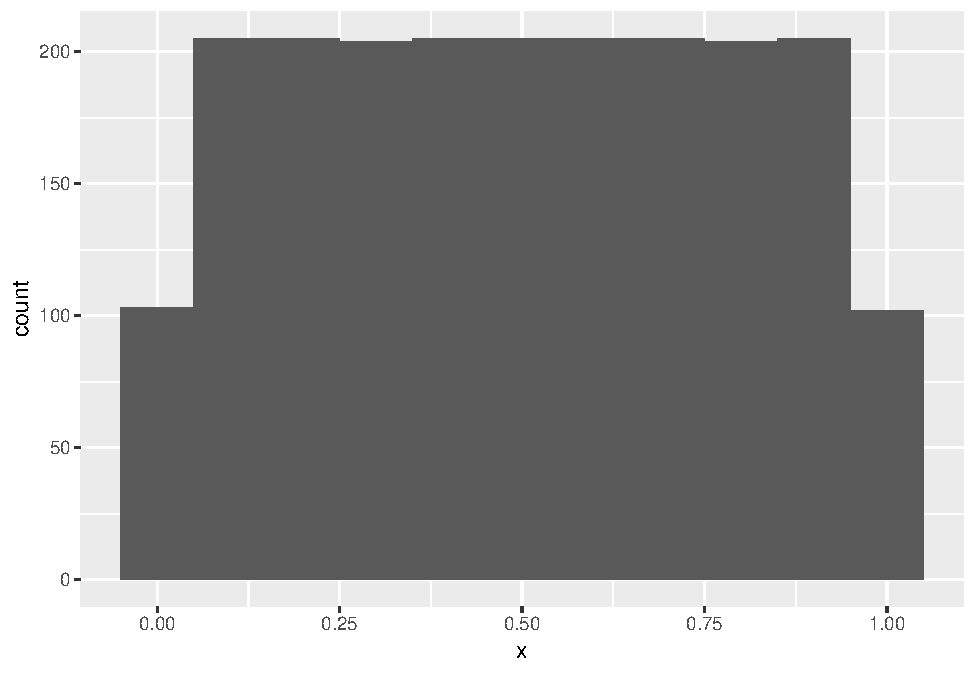
\includegraphics{stt-301-programming_files/figure-latex/unnamed-chunk-148-1.pdf}

Being able to provide a seed is important for repeatability of
simulations. The \texttt{set.seed()} function in R provides this
capability

\begin{Shaded}
\begin{Highlighting}[]
\KeywordTok{set.seed}\NormalTok{(}\DecValTok{123}\NormalTok{)}
\KeywordTok{runif}\NormalTok{(}\DecValTok{5}\NormalTok{)}
\end{Highlighting}
\end{Shaded}

\begin{verbatim}
## [1] 0.2875775 0.7883051 0.4089769 0.8830174 0.9404673
\end{verbatim}

\begin{Shaded}
\begin{Highlighting}[]
\KeywordTok{set.seed}\NormalTok{(}\DecValTok{123}\NormalTok{)}
\KeywordTok{runif}\NormalTok{(}\DecValTok{5}\NormalTok{)}
\end{Highlighting}
\end{Shaded}

\begin{verbatim}
## [1] 0.2875775 0.7883051 0.4089769 0.8830174 0.9404673
\end{verbatim}

\begin{Shaded}
\begin{Highlighting}[]
\KeywordTok{runif}\NormalTok{(}\DecValTok{5}\NormalTok{)}
\end{Highlighting}
\end{Shaded}

\begin{verbatim}
## [1] 0.0455565 0.5281055 0.8924190 0.5514350 0.4566147
\end{verbatim}

\subsection{8.2 Simulating from standard
distributions}\label{simulating-from-standard-distributions}

For example suppose that we want to generate coin flips, i.e., to
generate from a Bernoulli (0.5) distribution. Here is one way to do
this.

\begin{Shaded}
\begin{Highlighting}[]
\NormalTok{generate_coin <-}\StringTok{ }\ControlFlowTok{function}\NormalTok{(n) \{}
\NormalTok{    out <-}\StringTok{ }\KeywordTok{rep}\NormalTok{(}\DecValTok{0}\NormalTok{, n)}
\NormalTok{    out[}\KeywordTok{runif}\NormalTok{(n) }\OperatorTok{>}\StringTok{ }\FloatTok{0.5}\NormalTok{] <-}\StringTok{ }\DecValTok{1}
    \KeywordTok{return}\NormalTok{(out)}
\NormalTok{\}}
\KeywordTok{generate_coin}\NormalTok{(}\DecValTok{10}\NormalTok{)}
\end{Highlighting}
\end{Shaded}

\begin{verbatim}
##  [1] 1 0 1 1 0 1 0 0 0 1
\end{verbatim}

If we wanted H and T for heads and tails, a similar method would work.

\begin{Shaded}
\begin{Highlighting}[]
\NormalTok{generate_coin <-}\StringTok{ }\ControlFlowTok{function}\NormalTok{(n) \{}
\NormalTok{    out <-}\StringTok{ }\KeywordTok{rep}\NormalTok{(}\StringTok{"T"}\NormalTok{, n)}
\NormalTok{    out[}\KeywordTok{runif}\NormalTok{(n) }\OperatorTok{>}\StringTok{ }\FloatTok{0.5}\NormalTok{] <-}\StringTok{ "H"}
    \KeywordTok{return}\NormalTok{(out)}
\NormalTok{\}}
\KeywordTok{generate_coin}\NormalTok{(}\DecValTok{10}\NormalTok{)}
\end{Highlighting}
\end{Shaded}

\begin{verbatim}
##  [1] "H" "H" "H" "H" "H" "H" "H" "H" "T" "T"
\end{verbatim}

R provides functions that give the density (or mass function),
cumulative distribution function, quantile function, and generate
values.

\begin{enumerate}
\def\labelenumi{\arabic{enumi}.}
\tightlist
\item
  \texttt{dnorm} is the normal density function
\item
  \texttt{pnorm} is the normal cumulative distribution function
\item
  \texttt{qnorm} is the normal quantile function
\item
  \texttt{rnorm} generates values from a normal distribution
\end{enumerate}

Rather than designing our own methods for simulating from these
distributions, it is better to use the built in functions.

\begin{Shaded}
\begin{Highlighting}[]
\CommentTok{# 10 values from the N(100, 2) distribution}
\KeywordTok{rnorm}\NormalTok{(}\DecValTok{10}\NormalTok{, }\DataTypeTok{mean =} \DecValTok{100}\NormalTok{, }\DataTypeTok{sd =} \DecValTok{2}\NormalTok{)}
\end{Highlighting}
\end{Shaded}

\begin{verbatim}
##  [1] 103.57383 100.99570  96.06677 101.40271  99.05442  97.86435  99.56405
##  [8]  97.94799  98.54222  98.74992
\end{verbatim}

\begin{Shaded}
\begin{Highlighting}[]
\CommentTok{# 5 values from the Uniform(-3, 4) distribution}
\KeywordTok{runif}\NormalTok{(}\DecValTok{5}\NormalTok{, }\DataTypeTok{min =} \OperatorTok{-}\DecValTok{3}\NormalTok{, }\DataTypeTok{max =} \DecValTok{4}\NormalTok{)}
\end{Highlighting}
\end{Shaded}

\begin{verbatim}
## [1] -2.67918183  0.09540052  2.59247392 -2.14670518  0.92663589
\end{verbatim}

\begin{Shaded}
\begin{Highlighting}[]
\CommentTok{# 7 values from the binomial(10, 0.2) distribution}
\KeywordTok{rbinom}\NormalTok{(}\DecValTok{7}\NormalTok{, }\DataTypeTok{size =} \DecValTok{10}\NormalTok{, }\DataTypeTok{p =} \FloatTok{0.2}\NormalTok{)}
\end{Highlighting}
\end{Shaded}

\begin{verbatim}
## [1] 1 1 3 4 1 2 0
\end{verbatim}

In addition, the sample function provides a way to sample from a finite
population.

\begin{Shaded}
\begin{Highlighting}[]
\CommentTok{# 10 coin flips}
\KeywordTok{sample}\NormalTok{(}\KeywordTok{c}\NormalTok{(}\StringTok{"H"}\NormalTok{, }\StringTok{"T"}\NormalTok{), }\DecValTok{10}\NormalTok{, }\DataTypeTok{replace =} \OtherTok{TRUE}\NormalTok{)}
\end{Highlighting}
\end{Shaded}

\begin{verbatim}
##  [1] "H" "H" "T" "H" "T" "T" "T" "H" "T" "T"
\end{verbatim}

\begin{Shaded}
\begin{Highlighting}[]
\CommentTok{# a random permutation}
\KeywordTok{sample}\NormalTok{(}\DecValTok{1}\OperatorTok{:}\DecValTok{9}\NormalTok{, }\DecValTok{9}\NormalTok{, }\DataTypeTok{replace =} \OtherTok{FALSE}\NormalTok{)}
\end{Highlighting}
\end{Shaded}

\begin{verbatim}
## [1] 7 1 4 2 6 3 5 8 9
\end{verbatim}

\begin{Shaded}
\begin{Highlighting}[]
\CommentTok{# sample from a distribution with P(X=2) = 0.3; P(X=3)=0.5;  and P(X=17)=0.2}
\KeywordTok{sample}\NormalTok{(}\KeywordTok{c}\NormalTok{(}\DecValTok{2}\NormalTok{, }\DecValTok{3}\NormalTok{, }\DecValTok{17}\NormalTok{), }\DataTypeTok{size =} \DecValTok{15}\NormalTok{, }\DataTypeTok{replace =} \OtherTok{TRUE}\NormalTok{, }\DataTypeTok{prob =} \KeywordTok{c}\NormalTok{(}\FloatTok{0.3}\NormalTok{, }\FloatTok{0.5}\NormalTok{, }\FloatTok{0.2}\NormalTok{))}
\end{Highlighting}
\end{Shaded}

\begin{verbatim}
##  [1]  2  3  2  3  3 17 17 17  3  3  2  3  2  3  3
\end{verbatim}

\subsection{\texorpdfstring{8.3 Investigating \texttt{t}
tests}{8.3 Investigating t tests}}\label{investigating-t-tests}

Inverse CDF method (Inverse Transform Sampling)

Let X be our random variable of interest and assume X has CDF,
\(F_x(x)\)

GOAL: Generate random varibles from X

ALGORITHM 1. Generate \(U=Unif(0, 1)\) 2. Find x such that
\(F_x(x) = U\) =\textgreater{} \(x = F_x^-1 (U)\)

Theorem: Let X have continous CDF and define the variable Y such that
\(Y=Unif(0,1)\) \(Y = F_x(x)\) Then \(Y = Unif(0,1)\)

Proof: \(P(Y=< y)\) = \(P(F_x(x) =<y)\)

Solve: \(x_1 = F_x^-1 (U_i)\) U is uniform \(1-e^(z/x_1) = U_\)
\(-e^(-z/x_i) = u_i -1\) \(x_i = -zln(i-u_i)\)

You can control random number generation with \texttt{set.seed()}. R
uses Mersenne Twitter algorithm to generate random numbers based off the
seed

An Example: Algorithm 1. Select a seed 2. Multiply the seed by itself 3.
Output the middle number 4. Use the result as the new seed

\begin{Shaded}
\begin{Highlighting}[]
\NormalTok{seed =}\StringTok{ }\DecValTok{14}
\NormalTok{seed }\OperatorTok{*}\StringTok{ }\NormalTok{seed }\CommentTok{# 196 -> 19}
\end{Highlighting}
\end{Shaded}

\begin{verbatim}
## [1] 196
\end{verbatim}

\begin{Shaded}
\begin{Highlighting}[]
\DecValTok{19} \OperatorTok{*}\StringTok{ }\DecValTok{19} \CommentTok{# 361 -> 36}
\end{Highlighting}
\end{Shaded}

\begin{verbatim}
## [1] 361
\end{verbatim}

\begin{Shaded}
\begin{Highlighting}[]
\DecValTok{36} \OperatorTok{*}\StringTok{ }\DecValTok{36} \CommentTok{# 1296 - 29}
\end{Highlighting}
\end{Shaded}

\begin{verbatim}
## [1] 1296
\end{verbatim}

\section{9.0 Classifcation}\label{classifcation}

Classifcation methods are both extremely useful and an active area of
research in statistics. In this chapter we will learn about two common,
and somewhat different, classification methods, logistic regression and
k nearest neighbors

\subsection{9.1 Logistic regression}\label{logistic-regression}

We would like to predict the value of Y based on the value of the
predictor X. Let \texttt{p(X)\ =\ P(Y\ =\ 1jX)}. We will model
\texttt{p(X)} with the logistic function, which takes values between
\texttt{0} and \texttt{1}, which is of course appropriate for modeling a
probability:

\begin{Shaded}
\begin{Highlighting}[]
\KeywordTok{library}\NormalTok{(ggplot2)}
\NormalTok{logistic <-}\StringTok{ }\ControlFlowTok{function}\NormalTok{(x) \{}
    \KeywordTok{exp}\NormalTok{(x)}\OperatorTok{/}\NormalTok{(}\DecValTok{1} \OperatorTok{+}\StringTok{ }\KeywordTok{exp}\NormalTok{(x))}
\NormalTok{\}}
\KeywordTok{ggplot}\NormalTok{(}\KeywordTok{data.frame}\NormalTok{(}\DataTypeTok{x =} \KeywordTok{c}\NormalTok{(}\OperatorTok{-}\DecValTok{6}\NormalTok{, }\DecValTok{6}\NormalTok{)), }\KeywordTok{aes}\NormalTok{(x)) }\OperatorTok{+}\StringTok{ }\KeywordTok{stat_function}\NormalTok{(}\DataTypeTok{fun =}\NormalTok{ logistic)}
\end{Highlighting}
\end{Shaded}

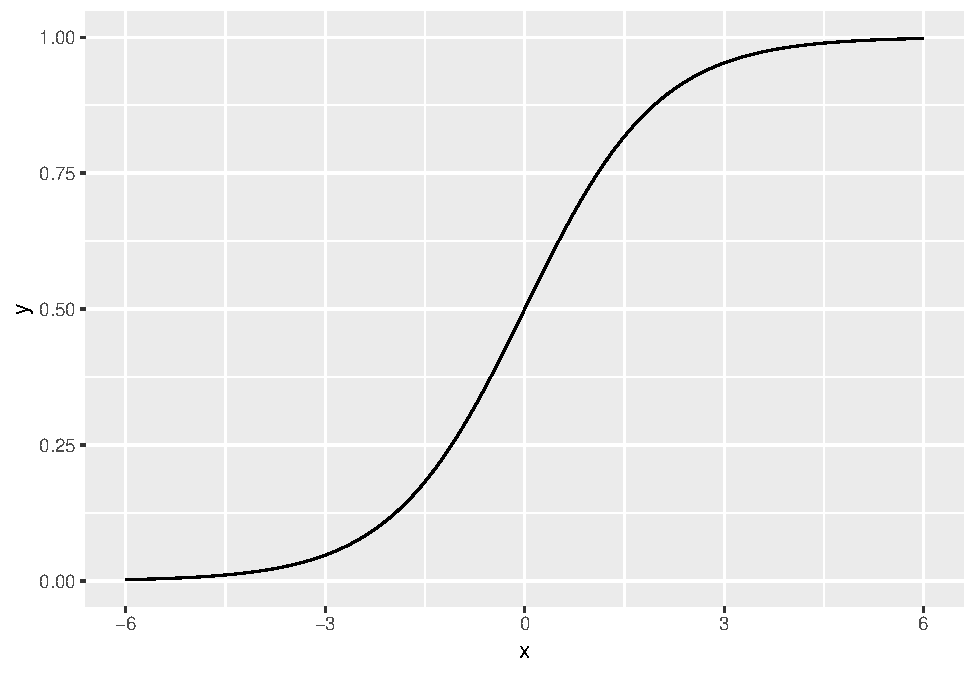
\includegraphics{stt-301-programming_files/figure-latex/unnamed-chunk-155-1.pdf}

\begin{Shaded}
\begin{Highlighting}[]
\KeywordTok{library}\NormalTok{(MASS)}
\end{Highlighting}
\end{Shaded}

\begin{verbatim}
## 
## Attaching package: 'MASS'
\end{verbatim}

\begin{verbatim}
## The following object is masked from 'package:dplyr':
## 
##     select
\end{verbatim}

\begin{Shaded}
\begin{Highlighting}[]
\KeywordTok{head}\NormalTok{(Pima.tr)}
\end{Highlighting}
\end{Shaded}

\begin{verbatim}
##   npreg glu bp skin  bmi   ped age type
## 1     5  86 68   28 30.2 0.364  24   No
## 2     7 195 70   33 25.1 0.163  55  Yes
## 3     5  77 82   41 35.8 0.156  35   No
## 4     0 165 76   43 47.9 0.259  26   No
## 5     0 107 60   25 26.4 0.133  23   No
## 6     5  97 76   27 35.6 0.378  52  Yes
\end{verbatim}

It will be more convenient to code the presence or absence of diabetes
by 1 and 0, so we first create another column in the data frame with
this coding:

\begin{Shaded}
\begin{Highlighting}[]
\NormalTok{Pima.tr}\OperatorTok{$}\NormalTok{diabetes <-}\StringTok{ }\KeywordTok{rep}\NormalTok{(}\DecValTok{0}\NormalTok{, }\KeywordTok{dim}\NormalTok{(Pima.tr)[}\DecValTok{1}\NormalTok{])}
\NormalTok{Pima.tr}\OperatorTok{$}\NormalTok{diabetes[Pima.tr}\OperatorTok{$}\NormalTok{type }\OperatorTok{==}\StringTok{ "Yes"}\NormalTok{] <-}\StringTok{ }\DecValTok{1}
\KeywordTok{head}\NormalTok{(Pima.tr)}
\end{Highlighting}
\end{Shaded}

\begin{verbatim}
##   npreg glu bp skin  bmi   ped age type diabetes
## 1     5  86 68   28 30.2 0.364  24   No        0
## 2     7 195 70   33 25.1 0.163  55  Yes        1
## 3     5  77 82   41 35.8 0.156  35   No        0
## 4     0 165 76   43 47.9 0.259  26   No        0
## 5     0 107 60   25 26.4 0.133  23   No        0
## 6     5  97 76   27 35.6 0.378  52  Yes        1
\end{verbatim}

In R we will use the function \texttt{glm} to fit logistic regression
models The \texttt{glm} function fits a wide variety of models.

To specify the logistic regression model we specify
\texttt{family\ =\ binomial} as an argument to glm.

\begin{enumerate}
\def\labelenumi{\arabic{enumi}.}
\tightlist
\item
  predictor and response variables
  \texttt{(diabetes\ \textasciitilde{}\ glu)}
\end{enumerate}

\begin{Shaded}
\begin{Highlighting}[]
\NormalTok{diabetes.lr1 <-}\StringTok{ }\KeywordTok{glm}\NormalTok{(diabetes }\OperatorTok{~}\StringTok{ }\NormalTok{glu, }\DataTypeTok{data =}\NormalTok{ Pima.tr, }\DataTypeTok{family =}\NormalTok{ binomial)}
\NormalTok{diabetes.lr1}
\end{Highlighting}
\end{Shaded}

\begin{verbatim}
## 
## Call:  glm(formula = diabetes ~ glu, family = binomial, data = Pima.tr)
## 
## Coefficients:
## (Intercept)          glu  
##    -5.50364      0.03778  
## 
## Degrees of Freedom: 199 Total (i.e. Null);  198 Residual
## Null Deviance:       256.4 
## Residual Deviance: 207.4     AIC: 211.4
\end{verbatim}

\begin{Shaded}
\begin{Highlighting}[]
\KeywordTok{summary}\NormalTok{(diabetes.lr1)}
\end{Highlighting}
\end{Shaded}

\begin{verbatim}
## 
## Call:
## glm(formula = diabetes ~ glu, family = binomial, data = Pima.tr)
## 
## Deviance Residuals: 
##     Min       1Q   Median       3Q      Max  
## -1.9714  -0.7795  -0.5292   0.8491   2.2633  
## 
## Coefficients:
##              Estimate Std. Error z value Pr(>|z|)    
## (Intercept) -5.503636   0.836077  -6.583 4.62e-11 ***
## glu          0.037784   0.006278   6.019 1.76e-09 ***
## ---
## Signif. codes:  0 '***' 0.001 '**' 0.01 '*' 0.05 '.' 0.1 ' ' 1
## 
## (Dispersion parameter for binomial family taken to be 1)
## 
##     Null deviance: 256.41  on 199  degrees of freedom
## Residual deviance: 207.37  on 198  degrees of freedom
## AIC: 211.37
## 
## Number of Fisher Scoring iterations: 4
\end{verbatim}

\begin{Shaded}
\begin{Highlighting}[]
\NormalTok{beta0.lr.}\DecValTok{1}\NormalTok{ <-}\StringTok{ }\KeywordTok{coef}\NormalTok{(diabetes.lr1)[}\DecValTok{1}\NormalTok{]}
\NormalTok{beta1.lr.}\DecValTok{1}\NormalTok{ <-}\StringTok{ }\KeywordTok{coef}\NormalTok{(diabetes.lr1)[}\DecValTok{2}\NormalTok{]}
\NormalTok{beta0.lr.}\DecValTok{1}
\end{Highlighting}
\end{Shaded}

\begin{verbatim}
## (Intercept) 
##   -5.503636
\end{verbatim}

\begin{Shaded}
\begin{Highlighting}[]
\NormalTok{beta1.lr.}\DecValTok{1}
\end{Highlighting}
\end{Shaded}

\begin{verbatim}
##        glu 
## 0.03778372
\end{verbatim}

The coefficients \texttt{b0} and \texttt{b1} are approximately
\texttt{b0} = -5.504 and \texttt{b1} = 0:038. So for example we can
estimate the probability that a woman in this population whose glucose
level is 150 would be diabetic as:

\begin{Shaded}
\begin{Highlighting}[]
\KeywordTok{exp}\NormalTok{(}\OperatorTok{-}\FloatTok{5.504} \OperatorTok{+}\StringTok{ }\FloatTok{0.038} \OperatorTok{*}\StringTok{ }\DecValTok{150}\NormalTok{)}\OperatorTok{/}\NormalTok{(}\DecValTok{1} \OperatorTok{+}\StringTok{ }\KeywordTok{exp}\NormalTok{(}\OperatorTok{-}\FloatTok{5.504} \OperatorTok{+}\StringTok{ }\FloatTok{0.038} \OperatorTok{*}\StringTok{ }\DecValTok{150}\NormalTok{))}
\end{Highlighting}
\end{Shaded}

\begin{verbatim}
## [1] 0.5488437
\end{verbatim}

We can plot the fitted probabilities along with the data
\texttt{by\ hand.}

\begin{Shaded}
\begin{Highlighting}[]
\NormalTok{diabetes.logistic.}\DecValTok{1}\NormalTok{ <-}\StringTok{ }\ControlFlowTok{function}\NormalTok{(x)\{}
    \KeywordTok{exp}\NormalTok{(beta0.lr.}\DecValTok{1} \OperatorTok{+}\StringTok{ }\NormalTok{beta1.lr.}\DecValTok{1} \OperatorTok{*}\StringTok{ }\NormalTok{x)}\OperatorTok{/}\NormalTok{(}\DecValTok{1} \OperatorTok{+}\StringTok{ }\KeywordTok{exp}\NormalTok{(beta0.lr.}\DecValTok{1} \OperatorTok{+}\StringTok{ }\NormalTok{beta1.lr.}\DecValTok{1} \OperatorTok{*}\StringTok{ }\NormalTok{x))}
\NormalTok{\}}
\KeywordTok{ggplot}\NormalTok{(Pima.tr, }\KeywordTok{aes}\NormalTok{(}\DataTypeTok{x =}\NormalTok{ glu, }\DataTypeTok{y =}\NormalTok{ diabetes)) }\OperatorTok{+}\StringTok{ }
\StringTok{    }\KeywordTok{stat_function}\NormalTok{(}\DataTypeTok{fun =}\NormalTok{ diabetes.logistic.}\DecValTok{1}\NormalTok{)}\OperatorTok{+}
\StringTok{    }\KeywordTok{geom_point}\NormalTok{()}
\end{Highlighting}
\end{Shaded}

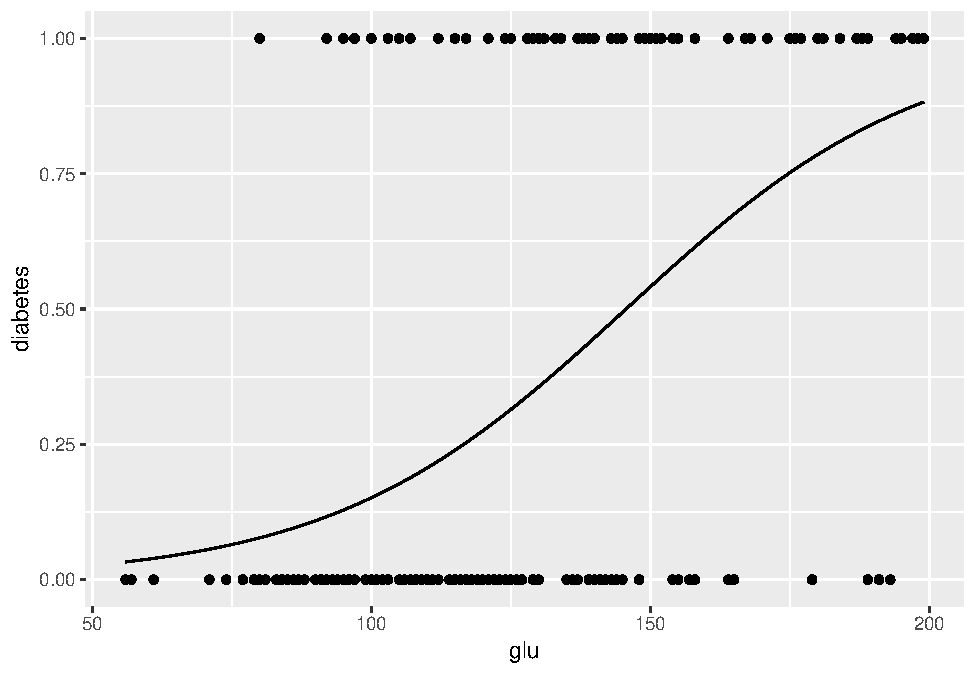
\includegraphics{stt-301-programming_files/figure-latex/unnamed-chunk-162-1.pdf}

The ggplot2 package also provides a way to do this more directly, using
\texttt{stat\_smooth}.

\begin{Shaded}
\begin{Highlighting}[]
\KeywordTok{ggplot}\NormalTok{(Pima.tr, }\KeywordTok{aes}\NormalTok{(}\DataTypeTok{x =}\NormalTok{ glu, }\DataTypeTok{y =}\NormalTok{ diabetes)) }\OperatorTok{+}
\StringTok{    }\KeywordTok{geom_point}\NormalTok{() }\OperatorTok{+}
\StringTok{    }\KeywordTok{stat_smooth}\NormalTok{(}\DataTypeTok{method =} \StringTok{"glm"}\NormalTok{, }\DataTypeTok{method.args =} \KeywordTok{list}\NormalTok{(}\DataTypeTok{family =} \StringTok{"binomial"}\NormalTok{), }\DataTypeTok{se =}\NormalTok{ F)}
\end{Highlighting}
\end{Shaded}

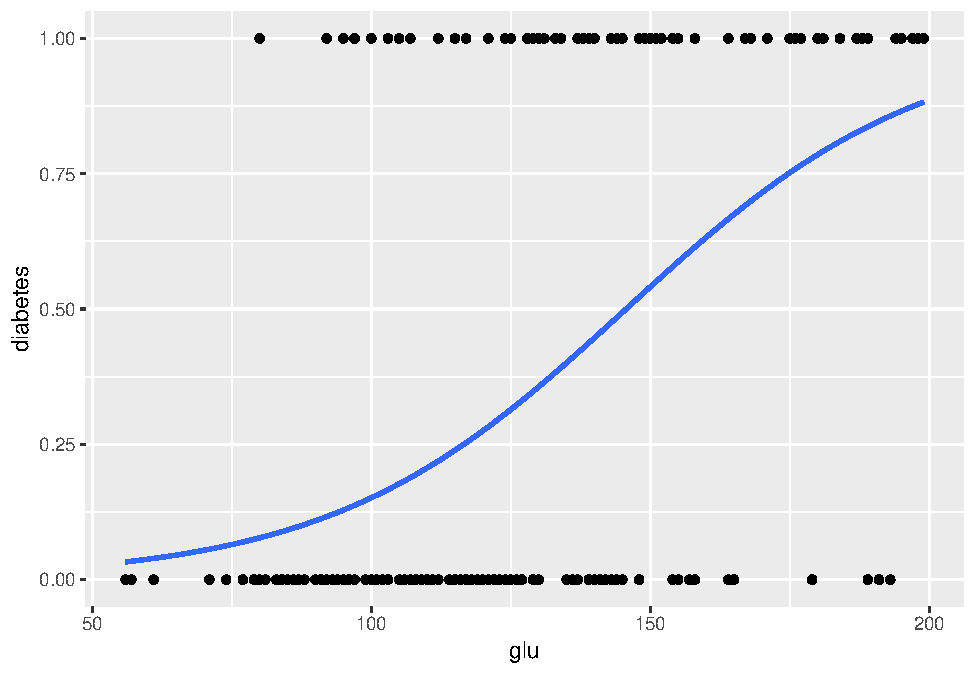
\includegraphics{stt-301-programming_files/figure-latex/unnamed-chunk-163-1.pdf}

From these graphics we can see that although glucose level and diabetes
are related, there are many women with high glucose levels who are not
diabetic, and many with low glucose levels who are diabetic, so likely
adding other predictors to the model will help.

\begin{Shaded}
\begin{Highlighting}[]
\KeywordTok{head}\NormalTok{(Pima.te)}
\end{Highlighting}
\end{Shaded}

\begin{verbatim}
##   npreg glu bp skin  bmi   ped age type
## 1     6 148 72   35 33.6 0.627  50  Yes
## 2     1  85 66   29 26.6 0.351  31   No
## 3     1  89 66   23 28.1 0.167  21   No
## 4     3  78 50   32 31.0 0.248  26  Yes
## 5     2 197 70   45 30.5 0.158  53  Yes
## 6     5 166 72   19 25.8 0.587  51  Yes
\end{verbatim}

\begin{Shaded}
\begin{Highlighting}[]
\NormalTok{diabetes.probs.}\DecValTok{1}\NormalTok{ <-}\StringTok{ }\KeywordTok{predict}\NormalTok{(diabetes.lr1, Pima.te, }\DataTypeTok{type =} \StringTok{"response"}\NormalTok{)}
\KeywordTok{head}\NormalTok{(diabetes.probs.}\DecValTok{1}\NormalTok{)}
\end{Highlighting}
\end{Shaded}

\begin{verbatim}
##          1          2          3          4          5          6 
## 0.52207428 0.09178605 0.10518608 0.07199064 0.87432542 0.68318799
\end{verbatim}

The predict function (with \texttt{type\ =\ "response"} specifed)
provides \texttt{p(x)\ =\ P(Y\ =\ 1jX\ =\ x)} for all the \texttt{x}
values in a data frame.

\begin{Shaded}
\begin{Highlighting}[]
\NormalTok{diabetes.predict.}\DecValTok{1}\NormalTok{ <-}\StringTok{ }\KeywordTok{rep}\NormalTok{(}\StringTok{"No"}\NormalTok{, }\KeywordTok{dim}\NormalTok{(Pima.te)[}\DecValTok{1}\NormalTok{])}
\NormalTok{diabetes.predict.}\DecValTok{1}\NormalTok{[diabetes.probs.}\DecValTok{1} \OperatorTok{>}\StringTok{ }\FloatTok{0.5}\NormalTok{] <-}\StringTok{ "Yes"}
\KeywordTok{head}\NormalTok{(diabetes.predict.}\DecValTok{1}\NormalTok{)}
\end{Highlighting}
\end{Shaded}

\begin{verbatim}
## [1] "Yes" "No"  "No"  "No"  "Yes" "Yes"
\end{verbatim}

\begin{Shaded}
\begin{Highlighting}[]
\KeywordTok{length}\NormalTok{(diabetes.predict.}\DecValTok{1}\NormalTok{[diabetes.predict.}\DecValTok{1} \OperatorTok{==}\StringTok{ }\NormalTok{Pima.te}\OperatorTok{$}\NormalTok{type])}\OperatorTok{/}\KeywordTok{dim}\NormalTok{(Pima.te)[}\DecValTok{1}\NormalTok{]}
\end{Highlighting}
\end{Shaded}

\begin{verbatim}
## [1] 0.7740964
\end{verbatim}

\subsubsection{9.1.1 Adding predictors}\label{adding-predictors}

We will next see how adding bmi, the body mass index, affects
predictions of diabetes.

\begin{Shaded}
\begin{Highlighting}[]
\NormalTok{diabetes.lr2 <-}\StringTok{ }\KeywordTok{glm}\NormalTok{(diabetes }\OperatorTok{~}\StringTok{ }\NormalTok{glu }\OperatorTok{+}\StringTok{ }\NormalTok{bmi, }\DataTypeTok{data =}\NormalTok{ Pima.tr, }\DataTypeTok{family =}\NormalTok{ binomial)}
\NormalTok{diabetes.lr2}
\end{Highlighting}
\end{Shaded}

\begin{verbatim}
## 
## Call:  glm(formula = diabetes ~ glu + bmi, family = binomial, data = Pima.tr)
## 
## Coefficients:
## (Intercept)          glu          bmi  
##    -8.21611      0.03572      0.09002  
## 
## Degrees of Freedom: 199 Total (i.e. Null);  197 Residual
## Null Deviance:       256.4 
## Residual Deviance: 198.5     AIC: 204.5
\end{verbatim}

\begin{Shaded}
\begin{Highlighting}[]
\KeywordTok{summary}\NormalTok{(diabetes.lr2)}
\end{Highlighting}
\end{Shaded}

\begin{verbatim}
## 
## Call:
## glm(formula = diabetes ~ glu + bmi, family = binomial, data = Pima.tr)
## 
## Deviance Residuals: 
##     Min       1Q   Median       3Q      Max  
## -2.0577  -0.7566  -0.4313   0.8011   2.2489  
## 
## Coefficients:
##              Estimate Std. Error z value Pr(>|z|)    
## (Intercept) -8.216106   1.346965  -6.100 1.06e-09 ***
## glu          0.035716   0.006311   5.659 1.52e-08 ***
## bmi          0.090016   0.031268   2.879  0.00399 ** 
## ---
## Signif. codes:  0 '***' 0.001 '**' 0.01 '*' 0.05 '.' 0.1 ' ' 1
## 
## (Dispersion parameter for binomial family taken to be 1)
## 
##     Null deviance: 256.41  on 199  degrees of freedom
## Residual deviance: 198.47  on 197  degrees of freedom
## AIC: 204.47
## 
## Number of Fisher Scoring iterations: 4
\end{verbatim}

\begin{Shaded}
\begin{Highlighting}[]
\NormalTok{diabetes.probs.}\DecValTok{2}\NormalTok{ <-}\StringTok{ }\KeywordTok{predict}\NormalTok{(diabetes.lr2, Pima.te, }\DataTypeTok{type =} \StringTok{"response"}\NormalTok{)}
\KeywordTok{head}\NormalTok{(diabetes.probs.}\DecValTok{2}\NormalTok{)}
\end{Highlighting}
\end{Shaded}

\begin{verbatim}
##          1          2          3          4          5          6 
## 0.52358599 0.05809584 0.07530477 0.06662362 0.82713369 0.50879270
\end{verbatim}

\begin{Shaded}
\begin{Highlighting}[]
\NormalTok{diabetes.predict.}\DecValTok{2}\NormalTok{ <-}\StringTok{ }\KeywordTok{rep}\NormalTok{(}\StringTok{"No"}\NormalTok{, }\KeywordTok{dim}\NormalTok{(Pima.te)[}\DecValTok{1}\NormalTok{])}
\NormalTok{diabetes.predict.}\DecValTok{2}\NormalTok{[diabetes.probs.}\DecValTok{2} \OperatorTok{>}\StringTok{ }\FloatTok{0.5}\NormalTok{] <-}\StringTok{ "Yes"}
\KeywordTok{head}\NormalTok{(diabetes.predict.}\DecValTok{2}\NormalTok{)}
\end{Highlighting}
\end{Shaded}

\begin{verbatim}
## [1] "Yes" "No"  "No"  "No"  "Yes" "Yes"
\end{verbatim}

\begin{Shaded}
\begin{Highlighting}[]
\KeywordTok{table}\NormalTok{(diabetes.predict.}\DecValTok{2}\NormalTok{, Pima.te}\OperatorTok{$}\NormalTok{type)}
\end{Highlighting}
\end{Shaded}

\begin{verbatim}
##                   
## diabetes.predict.2  No Yes
##                No  204  54
##                Yes  19  55
\end{verbatim}

\begin{Shaded}
\begin{Highlighting}[]
\KeywordTok{length}\NormalTok{(diabetes.predict.}\DecValTok{2}\NormalTok{[diabetes.predict.}\DecValTok{2} \OperatorTok{==}\StringTok{ }\NormalTok{Pima.te}\OperatorTok{$}\NormalTok{type])}\OperatorTok{/}\KeywordTok{dim}\NormalTok{(Pima.te)[}\DecValTok{1}\NormalTok{]}
\end{Highlighting}
\end{Shaded}

\begin{verbatim}
## [1] 0.7801205
\end{verbatim}

Adding bmi as a predictor did not improve the predictions by very much!

\begin{Shaded}
\begin{Highlighting}[]
\NormalTok{lr.int <-}\StringTok{ }\OperatorTok{-}\KeywordTok{coef}\NormalTok{(diabetes.lr2)[}\DecValTok{1}\NormalTok{]}\OperatorTok{/}\KeywordTok{coef}\NormalTok{(diabetes.lr2)[}\DecValTok{3}\NormalTok{]}
\NormalTok{lr.slope <-}\StringTok{ }\OperatorTok{-}\KeywordTok{coef}\NormalTok{(diabetes.lr2)[}\DecValTok{2}\NormalTok{]}\OperatorTok{/}\KeywordTok{coef}\NormalTok{(diabetes.lr2)[}\DecValTok{3}\NormalTok{]}
\KeywordTok{ggplot}\NormalTok{(Pima.tr, }\KeywordTok{aes}\NormalTok{(}\DataTypeTok{x =}\NormalTok{ glu, }\DataTypeTok{y =}\NormalTok{ bmi)) }\OperatorTok{+}\StringTok{ }\KeywordTok{geom_point}\NormalTok{(}\KeywordTok{aes}\NormalTok{(}\DataTypeTok{color =}\NormalTok{ type)) }\OperatorTok{+}
\StringTok{    }\KeywordTok{geom_abline}\NormalTok{(}\DataTypeTok{intercept =}\NormalTok{ lr.int, }\DataTypeTok{slope =}\NormalTok{ lr.slope)}
\end{Highlighting}
\end{Shaded}

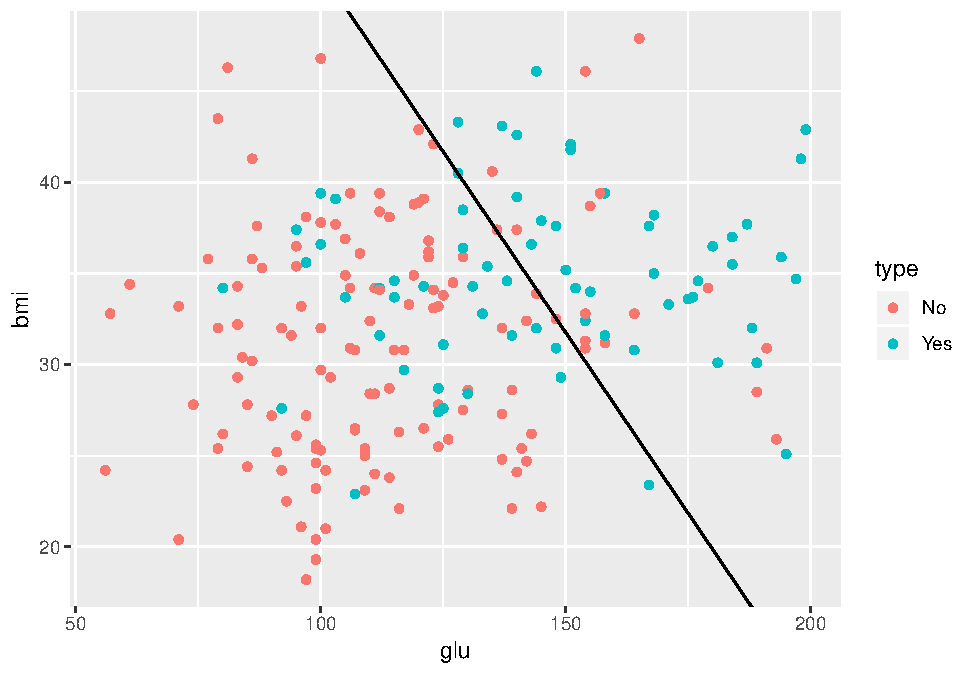
\includegraphics{stt-301-programming_files/figure-latex/unnamed-chunk-174-1.pdf}

\subsubsection{9.1.2 More than two classes}\label{more-than-two-classes}

Logistic regression methods also are applicable to classification
contexts where there are more than two classes. Consider for example
Fisher's iris data.

\begin{Shaded}
\begin{Highlighting}[]
\KeywordTok{data}\NormalTok{(iris)}
\KeywordTok{head}\NormalTok{(iris)}
\end{Highlighting}
\end{Shaded}

\begin{verbatim}
##   Sepal.Length Sepal.Width Petal.Length Petal.Width Species
## 1          5.1         3.5          1.4         0.2  setosa
## 2          4.9         3.0          1.4         0.2  setosa
## 3          4.7         3.2          1.3         0.2  setosa
## 4          4.6         3.1          1.5         0.2  setosa
## 5          5.0         3.6          1.4         0.2  setosa
## 6          5.4         3.9          1.7         0.4  setosa
\end{verbatim}

\begin{Shaded}
\begin{Highlighting}[]
\KeywordTok{ggplot}\NormalTok{(}\DataTypeTok{data =}\NormalTok{ iris, }\KeywordTok{aes}\NormalTok{(}\DataTypeTok{x =}\NormalTok{ Sepal.Length, }\DataTypeTok{y =}\NormalTok{ Sepal.Width)) }\OperatorTok{+}
\StringTok{    }\KeywordTok{geom_point}\NormalTok{(}\KeywordTok{aes}\NormalTok{(}\DataTypeTok{color =}\NormalTok{ Species))}
\end{Highlighting}
\end{Shaded}

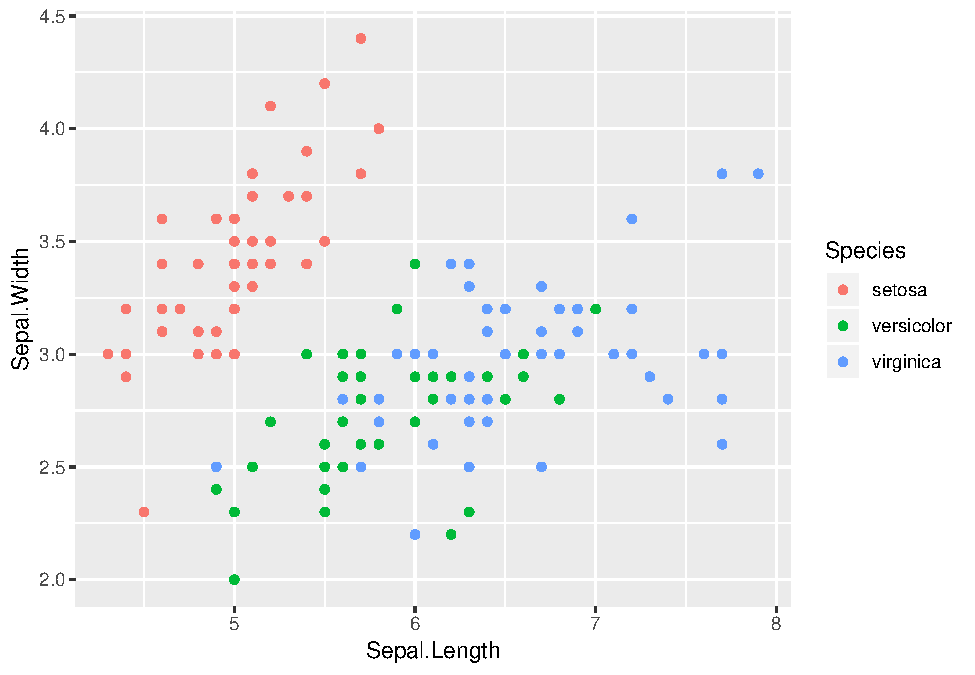
\includegraphics{stt-301-programming_files/figure-latex/unnamed-chunk-176-1.pdf}

\begin{Shaded}
\begin{Highlighting}[]
\KeywordTok{ggplot}\NormalTok{(}\DataTypeTok{data =}\NormalTok{ iris, }\KeywordTok{aes}\NormalTok{(}\DataTypeTok{x =}\NormalTok{ Petal.Length, }\DataTypeTok{y =}\NormalTok{ Petal.Width)) }\OperatorTok{+}
\StringTok{    }\KeywordTok{geom_point}\NormalTok{(}\KeywordTok{aes}\NormalTok{(}\DataTypeTok{color =}\NormalTok{ Species))}
\end{Highlighting}
\end{Shaded}

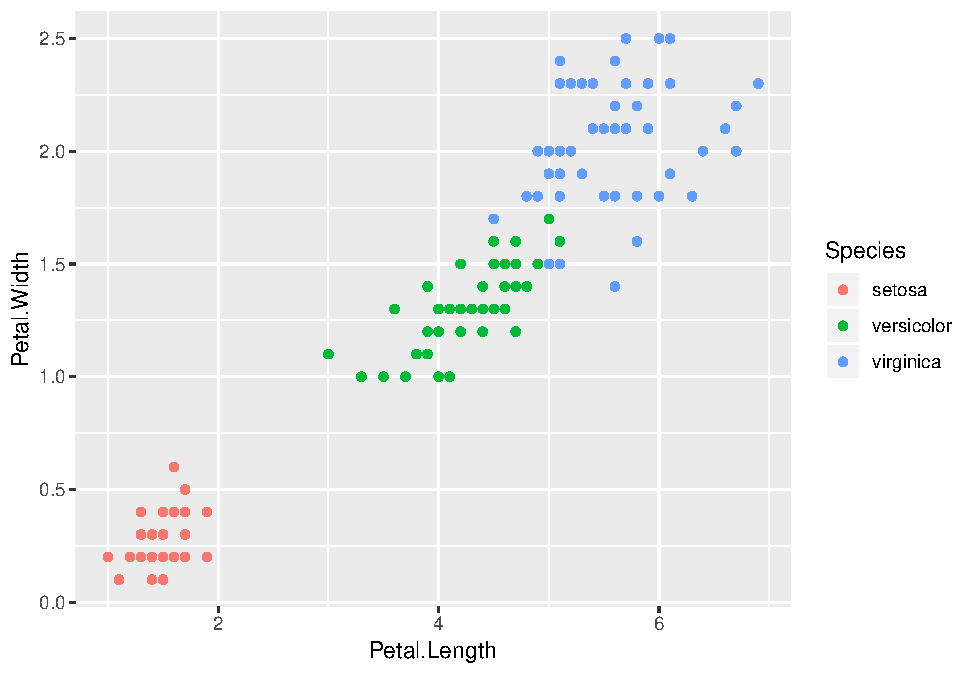
\includegraphics{stt-301-programming_files/figure-latex/unnamed-chunk-177-1.pdf}

Here the potential predictors are sepal width and length and petal width
and length, and the goal is to find a classifier that will yield the
correct species.

Before doing that we randomly choose 75 of the 150 rows of the data
frame to be the training sample, with the other 75 being the test
sample.

\begin{Shaded}
\begin{Highlighting}[]
\KeywordTok{set.seed}\NormalTok{(}\DecValTok{321}\NormalTok{)}
\NormalTok{selected <-}\StringTok{ }\KeywordTok{sample}\NormalTok{(}\DecValTok{1}\OperatorTok{:}\DecValTok{150}\NormalTok{, }\DataTypeTok{replace =} \OtherTok{FALSE}\NormalTok{, }\DataTypeTok{size =} \DecValTok{75}\NormalTok{)}
\NormalTok{iris.train <-}\StringTok{ }\NormalTok{iris[selected, ]}
\NormalTok{iris.test <-}\StringTok{ }\NormalTok{iris[}\OperatorTok{-}\NormalTok{selected, ]}
\end{Highlighting}
\end{Shaded}

There are several packages which implement logistic regression for data
with more than two classes. We will use the VGAM package. The function
vglm within VGAM implements logistic regression (and much more).

\begin{Shaded}
\begin{Highlighting}[]
\KeywordTok{library}\NormalTok{(VGAM)}
\end{Highlighting}
\end{Shaded}

\begin{verbatim}
## Loading required package: stats4
\end{verbatim}

\begin{verbatim}
## Loading required package: splines
\end{verbatim}

\begin{verbatim}
## 
## Attaching package: 'VGAM'
\end{verbatim}

\begin{verbatim}
## The following object is masked _by_ '.GlobalEnv':
## 
##     logistic
\end{verbatim}

\begin{verbatim}
## The following object is masked from 'package:tidyr':
## 
##     fill
\end{verbatim}

\begin{Shaded}
\begin{Highlighting}[]
\NormalTok{iris.lr <-}\StringTok{ }\KeywordTok{vglm}\NormalTok{(Species }\OperatorTok{~}\StringTok{ }\NormalTok{Petal.Width }\OperatorTok{+}\StringTok{ }\NormalTok{Petal.Length, }\DataTypeTok{data =}\NormalTok{ iris.train, }\DataTypeTok{family =}\NormalTok{ multinomial)}
\end{Highlighting}
\end{Shaded}

\begin{verbatim}
## Warning in checkwz(wz, M = M, trace = trace, wzepsilon =
## control$wzepsilon): 6 diagonal elements of the working weights variable
## 'wz' have been replaced by 1.819e-12
\end{verbatim}

\begin{verbatim}
## Warning in checkwz(wz, M = M, trace = trace, wzepsilon =
## control$wzepsilon): 12 diagonal elements of the working weights variable
## 'wz' have been replaced by 1.819e-12
\end{verbatim}

\begin{verbatim}
## Warning in checkwz(wz, M = M, trace = trace, wzepsilon =
## control$wzepsilon): 14 diagonal elements of the working weights variable
## 'wz' have been replaced by 1.819e-12
\end{verbatim}

\begin{verbatim}
## Warning in checkwz(wz, M = M, trace = trace, wzepsilon =
## control$wzepsilon): 16 diagonal elements of the working weights variable
## 'wz' have been replaced by 1.819e-12

## Warning in checkwz(wz, M = M, trace = trace, wzepsilon =
## control$wzepsilon): 16 diagonal elements of the working weights variable
## 'wz' have been replaced by 1.819e-12
\end{verbatim}

\begin{verbatim}
## Warning in checkwz(wz, M = M, trace = trace, wzepsilon =
## control$wzepsilon): 22 diagonal elements of the working weights variable
## 'wz' have been replaced by 1.819e-12
\end{verbatim}

\begin{verbatim}
## Warning in checkwz(wz, M = M, trace = trace, wzepsilon =
## control$wzepsilon): 25 diagonal elements of the working weights variable
## 'wz' have been replaced by 1.819e-12
\end{verbatim}

\begin{verbatim}
## Warning in checkwz(wz, M = M, trace = trace, wzepsilon =
## control$wzepsilon): 28 diagonal elements of the working weights variable
## 'wz' have been replaced by 1.819e-12
\end{verbatim}

\begin{verbatim}
## Warning in checkwz(wz, M = M, trace = trace, wzepsilon =
## control$wzepsilon): 31 diagonal elements of the working weights variable
## 'wz' have been replaced by 1.819e-12
\end{verbatim}

\begin{verbatim}
## Warning in checkwz(wz, M = M, trace = trace, wzepsilon =
## control$wzepsilon): 36 diagonal elements of the working weights variable
## 'wz' have been replaced by 1.819e-12
\end{verbatim}

\begin{verbatim}
## Warning in checkwz(wz, M = M, trace = trace, wzepsilon =
## control$wzepsilon): 37 diagonal elements of the working weights variable
## 'wz' have been replaced by 1.819e-12
\end{verbatim}

\begin{verbatim}
## Warning in checkwz(wz, M = M, trace = trace, wzepsilon =
## control$wzepsilon): 44 diagonal elements of the working weights variable
## 'wz' have been replaced by 1.819e-12
\end{verbatim}

\begin{verbatim}
## Warning in checkwz(wz, M = M, trace = trace, wzepsilon =
## control$wzepsilon): 45 diagonal elements of the working weights variable
## 'wz' have been replaced by 1.819e-12
\end{verbatim}

\begin{verbatim}
## Warning in checkwz(wz, M = M, trace = trace, wzepsilon =
## control$wzepsilon): 50 diagonal elements of the working weights variable
## 'wz' have been replaced by 1.819e-12
\end{verbatim}

\begin{verbatim}
## Warning in checkwz(wz, M = M, trace = trace, wzepsilon =
## control$wzepsilon): 54 diagonal elements of the working weights variable
## 'wz' have been replaced by 1.819e-12
\end{verbatim}

\begin{verbatim}
## Warning in vglm.fitter(x = x, y = y, w = w, offset = offset, Xm2 = Xm2, :
## convergence not obtained in 21 IRLS iterations
\end{verbatim}

\begin{Shaded}
\begin{Highlighting}[]
\KeywordTok{summary}\NormalTok{(iris.lr)}
\end{Highlighting}
\end{Shaded}

\begin{verbatim}
## 
## Call:
## vglm(formula = Species ~ Petal.Width + Petal.Length, family = multinomial, 
##     data = iris.train)
## 
## 
## Pearson residuals:
##                           Min         1Q    Median        3Q       Max
## log(mu[,1]/mu[,3]) -1.813e-06 -2.464e-07 4.360e-08 6.302e-08 1.644e-05
## log(mu[,2]/mu[,3]) -1.265e+00 -1.223e-04 6.589e-07 2.993e-03 2.471e+00
## 
## Coefficients: 
##                 Estimate Std. Error z value Pr(>|z|)
## (Intercept):1    118.947   9260.552      NA       NA
## (Intercept):2     63.510     34.004      NA       NA
## Petal.Width:1    -27.338  14731.810  -0.002    0.999
## Petal.Width:2    -14.554      7.466      NA       NA
## Petal.Length:1   -26.612   6453.201  -0.004    0.997
## Petal.Length:2    -8.242      5.591      NA       NA
## 
## Number of linear predictors:  2 
## 
## Names of linear predictors: log(mu[,1]/mu[,3]), log(mu[,2]/mu[,3])
## 
## Residual deviance: 8.6819 on 144 degrees of freedom
## 
## Log-likelihood: -4.341 on 144 degrees of freedom
## 
## Number of iterations: 21 
## 
## Warning: Hauck-Donner effect detected in the following estimate(s):
## '(Intercept):1', '(Intercept):2', 'Petal.Width:2', 'Petal.Length:2'
## 
## Reference group is level  3  of the response
\end{verbatim}

Notice that the family is specifed as \texttt{multinomial} rather than
\texttt{binomial} since we have more than two classes. When run with
these data, the \texttt{vglm} function returns several (about 20)
warnings. These occur mainly because the classes are so easily
separated, and are suppressed above.

Next we compute the probabilities for the test data.

\begin{Shaded}
\begin{Highlighting}[]
\NormalTok{iris.probs <-}\StringTok{ }\KeywordTok{predict}\NormalTok{(iris.lr, iris.test[, }\KeywordTok{c}\NormalTok{(}\DecValTok{3}\NormalTok{, }\DecValTok{4}\NormalTok{)], }\DataTypeTok{type =} \StringTok{"response"}\NormalTok{)}
\KeywordTok{head}\NormalTok{(iris.probs)}
\end{Highlighting}
\end{Shaded}

\begin{verbatim}
##    setosa   versicolor    virginica
## 4       1 1.003592e-11 1.129031e-32
## 5       1 1.598575e-12 7.887705e-34
## 9       1 1.598575e-12 7.887705e-34
## 11      1 1.003592e-11 1.129031e-32
## 12      1 6.300597e-11 1.616073e-31
## 14      1 1.799143e-15 1.747518e-38
\end{verbatim}

For these, we want to choose the highest probability in each row.

\begin{Shaded}
\begin{Highlighting}[]
\KeywordTok{which.max}\NormalTok{(}\KeywordTok{c}\NormalTok{(}\DecValTok{2}\NormalTok{, }\DecValTok{3}\NormalTok{, }\DecValTok{1}\NormalTok{, }\DecValTok{5}\NormalTok{, }\DecValTok{8}\NormalTok{, }\DecValTok{3}\NormalTok{))}
\end{Highlighting}
\end{Shaded}

\begin{verbatim}
## [1] 5
\end{verbatim}

\begin{Shaded}
\begin{Highlighting}[]
\KeywordTok{which.max}\NormalTok{(}\KeywordTok{c}\NormalTok{(}\DecValTok{2}\NormalTok{, }\DecValTok{20}\NormalTok{, }\DecValTok{4}\NormalTok{, }\DecValTok{5}\NormalTok{, }\DecValTok{9}\NormalTok{, }\DecValTok{1}\NormalTok{, }\DecValTok{0}\NormalTok{))}
\end{Highlighting}
\end{Shaded}

\begin{verbatim}
## [1] 2
\end{verbatim}

\begin{Shaded}
\begin{Highlighting}[]
\NormalTok{class.predictions <-}\StringTok{ }\KeywordTok{apply}\NormalTok{(iris.probs, }\DecValTok{1}\NormalTok{, which.max)}
\KeywordTok{head}\NormalTok{(class.predictions)}
\end{Highlighting}
\end{Shaded}

\begin{verbatim}
##  4  5  9 11 12 14 
##  1  1  1  1  1  1
\end{verbatim}

\begin{Shaded}
\begin{Highlighting}[]
\NormalTok{class.predictions[class.predictions }\OperatorTok{==}\StringTok{ }\DecValTok{1}\NormalTok{] <-}\StringTok{ }\KeywordTok{levels}\NormalTok{(iris}\OperatorTok{$}\NormalTok{Species)[}\DecValTok{1}\NormalTok{]}
\NormalTok{class.predictions[class.predictions }\OperatorTok{==}\StringTok{ }\DecValTok{2}\NormalTok{] <-}\StringTok{ }\KeywordTok{levels}\NormalTok{(iris}\OperatorTok{$}\NormalTok{Species)[}\DecValTok{2}\NormalTok{]}
\NormalTok{class.predictions[class.predictions }\OperatorTok{==}\StringTok{ }\DecValTok{3}\NormalTok{] <-}\StringTok{ }\KeywordTok{levels}\NormalTok{(iris}\OperatorTok{$}\NormalTok{Species)[}\DecValTok{3}\NormalTok{]}
\KeywordTok{head}\NormalTok{(class.predictions)}
\end{Highlighting}
\end{Shaded}

\begin{verbatim}
##        4        5        9       11       12       14 
## "setosa" "setosa" "setosa" "setosa" "setosa" "setosa"
\end{verbatim}

Next we create the confusion matrix.

\begin{Shaded}
\begin{Highlighting}[]
\KeywordTok{table}\NormalTok{(class.predictions, iris.test}\OperatorTok{$}\NormalTok{Species)}
\end{Highlighting}
\end{Shaded}

\begin{verbatim}
##                  
## class.predictions setosa versicolor virginica
##        setosa         26          0         0
##        versicolor      0         19         1
##        virginica       0          2        27
\end{verbatim}

\subsection{9.2 Nearest neighbor
methods}\label{nearest-neighbor-methods}

Nearest neighbor methods provide a rather different way to construct
classifiers, and have strengths (minimal assumptions, exible decision
boundaries) and weaknesses (computational burden, lack of
interpretability) compared to logistic regression models.

There are at least three R packages which implement \texttt{kNN},
including \texttt{class}, \texttt{kknn}, and \texttt{RWeka}. We will use
\texttt{class} below.

\begin{Shaded}
\begin{Highlighting}[]
\NormalTok{u.knn <-}\StringTok{ "http://blue.for.msu.edu/FOR875/data/knnExample.csv"}
\NormalTok{knnExample <-}\StringTok{ }\KeywordTok{read.csv}\NormalTok{(u.knn, }\DataTypeTok{header=}\OtherTok{TRUE}\NormalTok{)}
\KeywordTok{str}\NormalTok{(knnExample)}
\end{Highlighting}
\end{Shaded}

\begin{verbatim}
## 'data.frame':    200 obs. of  3 variables:
##  $ x1   : num  2.5261 0.367 0.7682 0.6934 -0.0198 ...
##  $ x2   : num  0.3211 0.0315 0.7175 0.7772 0.8673 ...
##  $ class: int  0 0 0 0 0 0 0 0 0 0 ...
\end{verbatim}

\begin{Shaded}
\begin{Highlighting}[]
\KeywordTok{ggplot}\NormalTok{(}\DataTypeTok{data =}\NormalTok{ knnExample, }\KeywordTok{aes}\NormalTok{(}\DataTypeTok{x =}\NormalTok{ x1, }\DataTypeTok{y =}\NormalTok{ x2)) }\OperatorTok{+}
\StringTok{    }\KeywordTok{geom_point}\NormalTok{(}\KeywordTok{aes}\NormalTok{(}\DataTypeTok{color =} \KeywordTok{as.factor}\NormalTok{(class))) }\OperatorTok{+}
\StringTok{    }\KeywordTok{theme_bw}\NormalTok{()}
\end{Highlighting}
\end{Shaded}

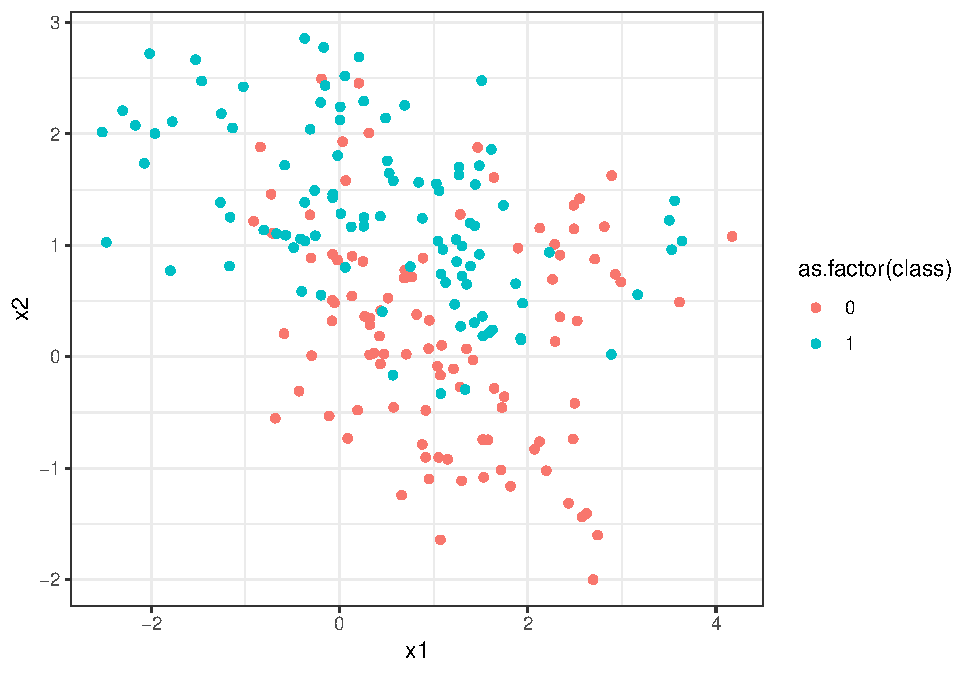
\includegraphics{stt-301-programming_files/figure-latex/unnamed-chunk-185-1.pdf}

\begin{Shaded}
\begin{Highlighting}[]
\KeywordTok{expand.grid}\NormalTok{(}\DataTypeTok{x =} \KeywordTok{c}\NormalTok{(}\DecValTok{1}\NormalTok{, }\DecValTok{2}\NormalTok{), }\DataTypeTok{y =} \KeywordTok{c}\NormalTok{(}\DecValTok{5}\NormalTok{, }\FloatTok{3.4}\NormalTok{, }\DecValTok{2}\NormalTok{))}
\end{Highlighting}
\end{Shaded}

\begin{verbatim}
##   x   y
## 1 1 5.0
## 2 2 5.0
## 3 1 3.4
## 4 2 3.4
## 5 1 2.0
## 6 2 2.0
\end{verbatim}

\begin{Shaded}
\begin{Highlighting}[]
\KeywordTok{min}\NormalTok{(knnExample}\OperatorTok{$}\NormalTok{x1)}
\end{Highlighting}
\end{Shaded}

\begin{verbatim}
## [1] -2.52082
\end{verbatim}

\begin{Shaded}
\begin{Highlighting}[]
\KeywordTok{max}\NormalTok{(knnExample}\OperatorTok{$}\NormalTok{x1)}
\end{Highlighting}
\end{Shaded}

\begin{verbatim}
## [1] 4.170746
\end{verbatim}

\begin{Shaded}
\begin{Highlighting}[]
\KeywordTok{min}\NormalTok{(knnExample}\OperatorTok{$}\NormalTok{x2)}
\end{Highlighting}
\end{Shaded}

\begin{verbatim}
## [1] -1.999853
\end{verbatim}

\begin{Shaded}
\begin{Highlighting}[]
\KeywordTok{max}\NormalTok{(knnExample}\OperatorTok{$}\NormalTok{x2)}
\end{Highlighting}
\end{Shaded}

\begin{verbatim}
## [1] 2.855805
\end{verbatim}

\begin{Shaded}
\begin{Highlighting}[]
\NormalTok{x.test <-}\StringTok{ }\KeywordTok{expand.grid}\NormalTok{(}\DataTypeTok{x1 =} \KeywordTok{seq}\NormalTok{(}\OperatorTok{-}\FloatTok{2.6}\NormalTok{, }\FloatTok{4.2}\NormalTok{, }\DataTypeTok{by =} \FloatTok{0.1}\NormalTok{), }\DataTypeTok{x2 =} \KeywordTok{seq}\NormalTok{(}\OperatorTok{-}\DecValTok{2}\NormalTok{, }\FloatTok{2.9}\NormalTok{, }\DataTypeTok{by =} \FloatTok{0.1}\NormalTok{))}
\end{Highlighting}
\end{Shaded}

\begin{Shaded}
\begin{Highlighting}[]
\KeywordTok{library}\NormalTok{(class)}
\NormalTok{Example_knn <-}\StringTok{ }\KeywordTok{knn}\NormalTok{(knnExample[, }\KeywordTok{c}\NormalTok{(}\DecValTok{1}\NormalTok{, }\DecValTok{2}\NormalTok{)], x.test, knnExample[,}\DecValTok{3}\NormalTok{], }\DataTypeTok{k =} \DecValTok{15}\NormalTok{, }\DataTypeTok{prob =} \OtherTok{TRUE}\NormalTok{)}
\NormalTok{prob <-}\StringTok{ }\KeywordTok{attr}\NormalTok{(Example_knn, }\StringTok{"prob"}\NormalTok{)}
\KeywordTok{head}\NormalTok{(prob)}
\end{Highlighting}
\end{Shaded}

\begin{verbatim}
## [1] 0.6666667 0.6666667 0.6666667 0.7333333 0.7333333 0.7333333
\end{verbatim}

\begin{Shaded}
\begin{Highlighting}[]
\NormalTok{train <-}\StringTok{ }\KeywordTok{rbind}\NormalTok{(iris3[}\DecValTok{1}\OperatorTok{:}\DecValTok{25}\NormalTok{,,}\DecValTok{1}\NormalTok{], iris3[}\DecValTok{1}\OperatorTok{:}\DecValTok{25}\NormalTok{,,}\DecValTok{2}\NormalTok{], iris3[}\DecValTok{1}\OperatorTok{:}\DecValTok{25}\NormalTok{,,}\DecValTok{3}\NormalTok{])}
\NormalTok{test <-}\StringTok{ }\KeywordTok{rbind}\NormalTok{(iris3[}\DecValTok{26}\OperatorTok{:}\DecValTok{50}\NormalTok{,,}\DecValTok{1}\NormalTok{], iris3[}\DecValTok{26}\OperatorTok{:}\DecValTok{50}\NormalTok{,,}\DecValTok{2}\NormalTok{], iris3[}\DecValTok{26}\OperatorTok{:}\DecValTok{50}\NormalTok{,,}\DecValTok{3}\NormalTok{])}
\NormalTok{cl <-}\StringTok{ }\KeywordTok{factor}\NormalTok{(}\KeywordTok{c}\NormalTok{(}\KeywordTok{rep}\NormalTok{(}\StringTok{"s"}\NormalTok{,}\DecValTok{25}\NormalTok{), }\KeywordTok{rep}\NormalTok{(}\StringTok{"c"}\NormalTok{,}\DecValTok{25}\NormalTok{), }\KeywordTok{rep}\NormalTok{(}\StringTok{"v"}\NormalTok{,}\DecValTok{25}\NormalTok{)))}
\KeywordTok{knn}\NormalTok{(train, test, cl, }\DataTypeTok{k =} \DecValTok{3}\NormalTok{, }\DataTypeTok{prob=}\OtherTok{TRUE}\NormalTok{)}
\end{Highlighting}
\end{Shaded}

\begin{verbatim}
##  [1] s s s s s s s s s s s s s s s s s s s s s s s s s c c v c c c c c v c
## [36] c c c c c c c c c c c c c c c v c c v v v v v c v v v v c v v v v v v
## [71] v v v v v
## attr(,"prob")
##  [1] 1.0000000 1.0000000 1.0000000 1.0000000 1.0000000 1.0000000 1.0000000
##  [8] 1.0000000 1.0000000 1.0000000 1.0000000 1.0000000 1.0000000 1.0000000
## [15] 1.0000000 1.0000000 1.0000000 1.0000000 1.0000000 1.0000000 1.0000000
## [22] 1.0000000 1.0000000 1.0000000 1.0000000 1.0000000 1.0000000 0.6666667
## [29] 1.0000000 1.0000000 1.0000000 1.0000000 1.0000000 0.6666667 1.0000000
## [36] 1.0000000 1.0000000 1.0000000 1.0000000 1.0000000 1.0000000 1.0000000
## [43] 1.0000000 1.0000000 1.0000000 1.0000000 1.0000000 1.0000000 1.0000000
## [50] 1.0000000 1.0000000 0.6666667 0.7500000 1.0000000 1.0000000 1.0000000
## [57] 1.0000000 1.0000000 0.5000000 1.0000000 1.0000000 1.0000000 1.0000000
## [64] 0.6666667 1.0000000 1.0000000 1.0000000 1.0000000 1.0000000 1.0000000
## [71] 1.0000000 0.6666667 1.0000000 1.0000000 0.6666667
## Levels: c s v
\end{verbatim}

\begin{Shaded}
\begin{Highlighting}[]
\KeywordTok{library}\NormalTok{(dplyr)}
\NormalTok{df1 <-}\StringTok{ }\KeywordTok{mutate}\NormalTok{(x.test, }\DataTypeTok{prob =}\NormalTok{ prob, }\DataTypeTok{class =} \DecValTok{0}\NormalTok{, }\DataTypeTok{prob_cls =} \KeywordTok{ifelse}\NormalTok{(Example_knn }\OperatorTok{==}\StringTok{ }\NormalTok{class, }\DecValTok{1}\NormalTok{, }\DecValTok{0}\NormalTok{))}
\KeywordTok{str}\NormalTok{(df1)}
\end{Highlighting}
\end{Shaded}

\begin{verbatim}
## 'data.frame':    3450 obs. of  5 variables:
##  $ x1      : num  -2.6 -2.5 -2.4 -2.3 -2.2 -2.1 -2 -1.9 -1.8 -1.7 ...
##  $ x2      : num  -2 -2 -2 -2 -2 -2 -2 -2 -2 -2 ...
##  $ prob    : num  0.667 0.667 0.667 0.733 0.733 ...
##  $ class   : num  0 0 0 0 0 0 0 0 0 0 ...
##  $ prob_cls: num  1 1 1 1 1 1 1 1 1 1 ...
\end{verbatim}

\begin{Shaded}
\begin{Highlighting}[]
\NormalTok{df2 <-}\StringTok{ }\KeywordTok{mutate}\NormalTok{(x.test, }\DataTypeTok{prob =}\NormalTok{ prob, }\DataTypeTok{class =} \DecValTok{1}\NormalTok{, }\DataTypeTok{prob_cls =} \KeywordTok{ifelse}\NormalTok{(Example_knn }\OperatorTok{==}\StringTok{ }\NormalTok{class, }\DecValTok{1}\NormalTok{, }\DecValTok{0}\NormalTok{))}
\NormalTok{bigdf <-}\StringTok{ }\KeywordTok{bind_rows}\NormalTok{(df1, df2)}

\KeywordTok{names}\NormalTok{(knnExample)}
\end{Highlighting}
\end{Shaded}

\begin{verbatim}
## [1] "x1"    "x2"    "class"
\end{verbatim}

\begin{Shaded}
\begin{Highlighting}[]
\KeywordTok{ggplot}\NormalTok{(bigdf) }\OperatorTok{+}\StringTok{ }
\StringTok{    }\KeywordTok{geom_point}\NormalTok{(}\KeywordTok{aes}\NormalTok{(}\DataTypeTok{x =}\NormalTok{ x1, }\DataTypeTok{y =}\NormalTok{ x2, }\DataTypeTok{col =}\NormalTok{ class),}\DataTypeTok{data =} \KeywordTok{mutate}\NormalTok{(x.test, }\DataTypeTok{class =}\NormalTok{ Example_knn), }\DataTypeTok{size =} \FloatTok{0.5}\NormalTok{) }\OperatorTok{+}
\StringTok{    }\KeywordTok{geom_point}\NormalTok{(}\KeywordTok{aes}\NormalTok{(}\DataTypeTok{x =}\NormalTok{ x1, }\DataTypeTok{y =}\NormalTok{ x2, }\DataTypeTok{col =} \KeywordTok{as.factor}\NormalTok{(class)), }\DataTypeTok{size =} \DecValTok{4}\NormalTok{, }\DataTypeTok{shape =} \DecValTok{1}\NormalTok{, }\DataTypeTok{data =}\NormalTok{ knnExample) }\OperatorTok{+}\StringTok{ }
\StringTok{    }\KeywordTok{geom_contour}\NormalTok{(}\KeywordTok{aes}\NormalTok{(}\DataTypeTok{x =}\NormalTok{ x1, }\DataTypeTok{y =}\NormalTok{ x2, }\DataTypeTok{z =}\NormalTok{ prob_cls, }\DataTypeTok{group =} \KeywordTok{as.factor}\NormalTok{(class), }\DataTypeTok{color =} \KeywordTok{as.factor}\NormalTok{(class)), }\DataTypeTok{size =} \DecValTok{1}\NormalTok{, }\DataTypeTok{bins =} \DecValTok{1}\NormalTok{, }\DataTypeTok{data =}\NormalTok{ bigdf) }\OperatorTok{+}\StringTok{ }
\StringTok{    }\KeywordTok{theme_bw}\NormalTok{()}
\end{Highlighting}
\end{Shaded}

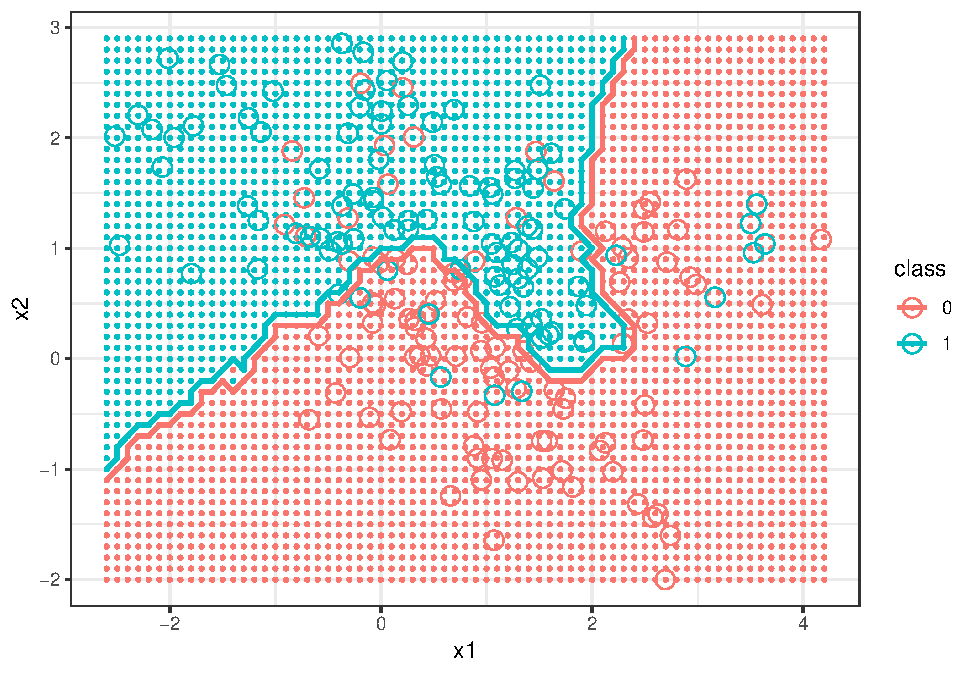
\includegraphics{stt-301-programming_files/figure-latex/unnamed-chunk-193-1.pdf}

\begin{Shaded}
\begin{Highlighting}[]
\NormalTok{Example_knn <-}\StringTok{ }\KeywordTok{knn}\NormalTok{(knnExample[, }\KeywordTok{c}\NormalTok{(}\DecValTok{1}\NormalTok{, }\DecValTok{2}\NormalTok{)], x.test, knnExample[,}\DecValTok{3}\NormalTok{], }\DataTypeTok{k =} \DecValTok{1}\NormalTok{, }\DataTypeTok{prob =} \OtherTok{TRUE}\NormalTok{) }
\NormalTok{prob <-}\StringTok{ }\KeywordTok{attr}\NormalTok{(Example_knn, }\StringTok{"prob"}\NormalTok{)}
\KeywordTok{head}\NormalTok{(prob)}
\end{Highlighting}
\end{Shaded}

\begin{verbatim}
## [1] 1 1 1 1 1 1
\end{verbatim}

\begin{Shaded}
\begin{Highlighting}[]
\NormalTok{df1 <-}\StringTok{ }\KeywordTok{mutate}\NormalTok{(x.test, }\DataTypeTok{prob =}\NormalTok{ prob, }\DataTypeTok{class =} \DecValTok{0}\NormalTok{, }\DataTypeTok{prob_cls =} \KeywordTok{ifelse}\NormalTok{(Example_knn }\OperatorTok{==}\StringTok{ }\NormalTok{class, }\DecValTok{1}\NormalTok{, }\DecValTok{0}\NormalTok{))}
\KeywordTok{str}\NormalTok{(df1)}
\end{Highlighting}
\end{Shaded}

\begin{verbatim}
## 'data.frame':    3450 obs. of  5 variables:
##  $ x1      : num  -2.6 -2.5 -2.4 -2.3 -2.2 -2.1 -2 -1.9 -1.8 -1.7 ...
##  $ x2      : num  -2 -2 -2 -2 -2 -2 -2 -2 -2 -2 ...
##  $ prob    : num  1 1 1 1 1 1 1 1 1 1 ...
##  $ class   : num  0 0 0 0 0 0 0 0 0 0 ...
##  $ prob_cls: num  1 1 1 1 1 1 1 1 1 1 ...
\end{verbatim}

\begin{Shaded}
\begin{Highlighting}[]
\NormalTok{df2 <-}\StringTok{ }\KeywordTok{mutate}\NormalTok{(x.test, }\DataTypeTok{prob =}\NormalTok{ prob, }\DataTypeTok{class =} \DecValTok{1}\NormalTok{, }\DataTypeTok{prob_cls =} \KeywordTok{ifelse}\NormalTok{(Example_knn }\OperatorTok{==}\StringTok{ }\NormalTok{class, }\DecValTok{1}\NormalTok{, }\DecValTok{0}\NormalTok{))}
\NormalTok{bigdf <-}\StringTok{ }\KeywordTok{bind_rows}\NormalTok{(df1, df2)}
\end{Highlighting}
\end{Shaded}

\begin{Shaded}
\begin{Highlighting}[]
\KeywordTok{ggplot}\NormalTok{(bigdf) }\OperatorTok{+}\StringTok{ }\KeywordTok{geom_point}\NormalTok{(}\KeywordTok{aes}\NormalTok{(}\DataTypeTok{x =}\NormalTok{ x1, }\DataTypeTok{y =}\NormalTok{ x2, }\DataTypeTok{col =}\NormalTok{ class), }\DataTypeTok{data =} \KeywordTok{mutate}\NormalTok{(x.test, }\DataTypeTok{class =}\NormalTok{ Example_knn), }\DataTypeTok{size =} \FloatTok{0.5}\NormalTok{) }\OperatorTok{+}
\StringTok{    }\KeywordTok{geom_point}\NormalTok{(}\KeywordTok{aes}\NormalTok{(}\DataTypeTok{x =}\NormalTok{ x1, }\DataTypeTok{y =}\NormalTok{ x2, }\DataTypeTok{col =} \KeywordTok{as.factor}\NormalTok{(class)), }\DataTypeTok{size =} \DecValTok{4}\NormalTok{, }\DataTypeTok{shape =} \DecValTok{1}\NormalTok{, }\DataTypeTok{data =}\NormalTok{ knnExample) }\OperatorTok{+}\StringTok{ }
\StringTok{    }\KeywordTok{geom_contour}\NormalTok{(}\KeywordTok{aes}\NormalTok{(}\DataTypeTok{x =}\NormalTok{ x1, }\DataTypeTok{y =}\NormalTok{ x2, }\DataTypeTok{z =}\NormalTok{ prob_cls, }\DataTypeTok{group =} \KeywordTok{as.factor}\NormalTok{(class), }\DataTypeTok{color =} \KeywordTok{as.factor}\NormalTok{(class)), }\DataTypeTok{size =} \DecValTok{1}\NormalTok{, }\DataTypeTok{bins =} \DecValTok{1}\NormalTok{, }\DataTypeTok{data =}\NormalTok{ bigdf) }\OperatorTok{+}\StringTok{ }
\StringTok{    }\KeywordTok{theme_bw}\NormalTok{()}
\end{Highlighting}
\end{Shaded}

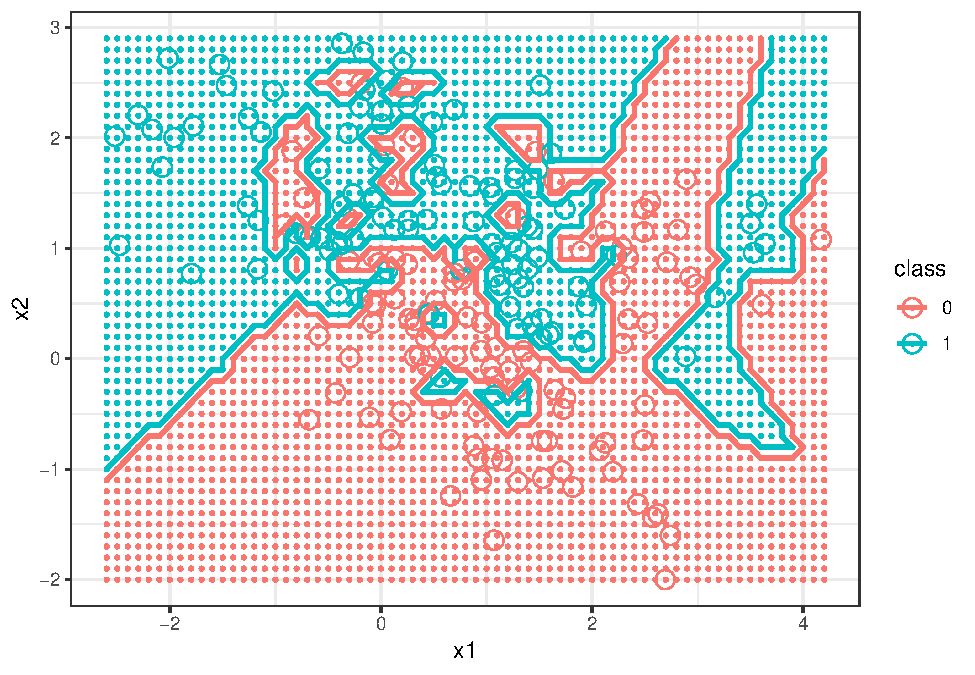
\includegraphics{stt-301-programming_files/figure-latex/unnamed-chunk-197-1.pdf}

\subsubsection{9.2.1 kNN and the diabetes
data}\label{knn-and-the-diabetes-data}

Next kNN is applied to the diabetes data. We will use the same
predictors, \texttt{glu} and \texttt{bmi} that were used in the logistic
regression example. Since the scales of the predictor variables are
substantially different, they are standardized first. The value
\texttt{k\ =\ 15} is chosen for kNN.

\begin{Shaded}
\begin{Highlighting}[]
\NormalTok{Pima.tr[, }\DecValTok{1}\OperatorTok{:}\DecValTok{7}\NormalTok{] <-}\StringTok{ }\KeywordTok{scale}\NormalTok{(Pima.tr[, }\DecValTok{1}\OperatorTok{:}\DecValTok{7}\NormalTok{], }\DataTypeTok{center =} \OtherTok{TRUE}\NormalTok{, }\DataTypeTok{scale =} \OtherTok{TRUE}\NormalTok{)}
\NormalTok{Pima.te[, }\DecValTok{1}\OperatorTok{:}\DecValTok{7}\NormalTok{] <-}\StringTok{ }\KeywordTok{scale}\NormalTok{(Pima.te[, }\DecValTok{1}\OperatorTok{:}\DecValTok{7}\NormalTok{], }\DataTypeTok{center =} \OtherTok{TRUE}\NormalTok{, }\DataTypeTok{scale =} \OtherTok{TRUE}\NormalTok{)}
\NormalTok{knn_Pima <-}\StringTok{ }\KeywordTok{knn}\NormalTok{(Pima.tr[, }\KeywordTok{c}\NormalTok{(}\DecValTok{2}\NormalTok{, }\DecValTok{5}\NormalTok{)], Pima.te[, }\KeywordTok{c}\NormalTok{(}\DecValTok{2}\NormalTok{, }\DecValTok{5}\NormalTok{)], Pima.tr[, }\DecValTok{8}\NormalTok{], }\DataTypeTok{k =} \DecValTok{15}\NormalTok{, }\DataTypeTok{prob =} \OtherTok{TRUE}\NormalTok{)}
\KeywordTok{table}\NormalTok{(knn_Pima, Pima.te[, }\DecValTok{8}\NormalTok{])}
\end{Highlighting}
\end{Shaded}

\begin{verbatim}
##         
## knn_Pima  No Yes
##      No  206  55
##      Yes  17  54
\end{verbatim}

\subsubsection{9.2.2 kNN and the iris data}\label{knn-and-the-iris-data}

Now kNN is used to classify the iris data. As before we use petal length
and width as predictors

\begin{Shaded}
\begin{Highlighting}[]
\KeywordTok{sd}\NormalTok{(iris.train}\OperatorTok{$}\NormalTok{Petal.Width)}
\end{Highlighting}
\end{Shaded}

\begin{verbatim}
## [1] 0.728585
\end{verbatim}

\begin{Shaded}
\begin{Highlighting}[]
\KeywordTok{sd}\NormalTok{(iris.train}\OperatorTok{$}\NormalTok{Petal.Length)}
\end{Highlighting}
\end{Shaded}

\begin{verbatim}
## [1] 1.671873
\end{verbatim}

\begin{Shaded}
\begin{Highlighting}[]
\KeywordTok{head}\NormalTok{(iris.train)}
\end{Highlighting}
\end{Shaded}

\begin{verbatim}
##     Sepal.Length Sepal.Width Petal.Length Petal.Width    Species
## 144          6.8         3.2          5.9         2.3  virginica
## 140          6.9         3.1          5.4         2.1  virginica
## 36           5.0         3.2          1.2         0.2     setosa
## 38           4.9         3.6          1.4         0.1     setosa
## 58           4.9         2.4          3.3         1.0 versicolor
## 50           5.0         3.3          1.4         0.2     setosa
\end{verbatim}

\begin{Shaded}
\begin{Highlighting}[]
\NormalTok{knn_iris <-}\StringTok{ }\KeywordTok{knn}\NormalTok{(iris.train[, }\KeywordTok{c}\NormalTok{(}\DecValTok{3}\NormalTok{, }\DecValTok{4}\NormalTok{)], iris.test[, }\KeywordTok{c}\NormalTok{(}\DecValTok{3}\NormalTok{, }\DecValTok{4}\NormalTok{)], iris.train[, }\DecValTok{5}\NormalTok{], }\DataTypeTok{k =} \DecValTok{1}\NormalTok{, }\DataTypeTok{prob =} \OtherTok{TRUE}\NormalTok{)}
\KeywordTok{table}\NormalTok{(knn_iris, iris.test[, }\DecValTok{5}\NormalTok{])}
\end{Highlighting}
\end{Shaded}

\begin{verbatim}
##             
## knn_iris     setosa versicolor virginica
##   setosa         26          0         0
##   versicolor      0         20         1
##   virginica       0          1        27
\end{verbatim}

\begin{Shaded}
\begin{Highlighting}[]
\NormalTok{knn_iris <-}\StringTok{ }\KeywordTok{knn}\NormalTok{(iris.train[, }\KeywordTok{c}\NormalTok{(}\DecValTok{3}\NormalTok{, }\DecValTok{4}\NormalTok{)], iris.test[, }\KeywordTok{c}\NormalTok{(}\DecValTok{3}\NormalTok{, }\DecValTok{4}\NormalTok{)], iris.train[, }\DecValTok{5}\NormalTok{], }\DataTypeTok{k =} \DecValTok{3}\NormalTok{, }\DataTypeTok{prob =} \OtherTok{TRUE}\NormalTok{)}
\KeywordTok{table}\NormalTok{(knn_iris, iris.test[, }\DecValTok{5}\NormalTok{])}
\end{Highlighting}
\end{Shaded}

\begin{verbatim}
##             
## knn_iris     setosa versicolor virginica
##   setosa         26          0         0
##   versicolor      0         19         1
##   virginica       0          2        27
\end{verbatim}

\begin{Shaded}
\begin{Highlighting}[]
\NormalTok{knn_iris <-}\StringTok{ }\KeywordTok{knn}\NormalTok{(iris.train[, }\KeywordTok{c}\NormalTok{(}\DecValTok{3}\NormalTok{, }\DecValTok{4}\NormalTok{)], iris.test[, }\KeywordTok{c}\NormalTok{(}\DecValTok{3}\NormalTok{, }\DecValTok{4}\NormalTok{)], iris.train[, }\DecValTok{5}\NormalTok{], }\DataTypeTok{k =} \DecValTok{15}\NormalTok{, }\DataTypeTok{prob=} \OtherTok{TRUE}\NormalTok{)}
\KeywordTok{table}\NormalTok{(knn_iris, iris.test[, }\DecValTok{5}\NormalTok{])}
\end{Highlighting}
\end{Shaded}

\begin{verbatim}
##             
## knn_iris     setosa versicolor virginica
##   setosa         26          0         0
##   versicolor      0         19         1
##   virginica       0          2        27
\end{verbatim}


\end{document}
